% Options for packages loaded elsewhere
\PassOptionsToPackage{unicode}{hyperref}
\PassOptionsToPackage{hyphens}{url}
\PassOptionsToPackage{dvipsnames,svgnames,x11names}{xcolor}
\documentclass[
]{report}
\usepackage{xcolor}
\usepackage[inner=1.25in,outer=0.85in,top=1in,bottom=1in]{geometry}
\usepackage{amsmath,amssymb}
\setcounter{secnumdepth}{-\maxdimen} % remove section numbering
\usepackage{iftex}
\ifPDFTeX
  \usepackage[T1]{fontenc}
  \usepackage[utf8]{inputenc}
  \usepackage{textcomp} % provide euro and other symbols
\else % if luatex or xetex
  \usepackage{unicode-math} % this also loads fontspec
  \defaultfontfeatures{Scale=MatchLowercase}
  \defaultfontfeatures[\rmfamily]{Ligatures=TeX,Scale=1}
\fi
\usepackage{lmodern}
\ifPDFTeX\else
  % xetex/luatex font selection
  \setmainfont[]{STIX Two Text}
  \setmonofont[BoldFont=DejaVuSansMono-Bold.ttf,ItalicFont=DejaVuSansMono-Oblique.ttf,BoldItalicFont=DejaVuSansMono-BoldOblique.ttf]{DejaVuSansMono.ttf}
\fi
% Use upquote if available, for straight quotes in verbatim environments
\IfFileExists{upquote.sty}{\usepackage{upquote}}{}
\IfFileExists{microtype.sty}{% use microtype if available
  \usepackage[]{microtype}
  \UseMicrotypeSet[protrusion]{basicmath} % disable protrusion for tt fonts
}{}
\makeatletter
\@ifundefined{KOMAClassName}{% if non-KOMA class
  \IfFileExists{parskip.sty}{%
    \usepackage{parskip}
  }{% else
    \setlength{\parindent}{0pt}
    \setlength{\parskip}{6pt plus 2pt minus 1pt}}
}{% if KOMA class
  \KOMAoptions{parskip=half}}
\makeatother
\setlength{\emergencystretch}{3em} % prevent overfull lines
\providecommand{\tightlist}{%
  \setlength{\itemsep}{0pt}\setlength{\parskip}{0pt}}
% Pandoc's template disables all heading numbering with
% \setcounter{secnumdepth}{-\maxdimen}.  Section numbers are typed by hand into
% the heading text (## 11.1  Measurement Fundamentals), but chapters are not, so
% re-enable numbering at the chapter level only.
\setcounter{secnumdepth}{0}

% fontspec/unicode-math commands exist only under XeTeX and LuaTeX; pandoc's
% own template guards its font selection the same way, so guard ours too rather
% than breaking a pdfTeX run outright.
\ifPDFTeX
  \newcommand{\mathsymfont}{}
\else
  % STIX Two Text is a variable font; fontspec cannot auto-detect the bold
  % weight, so we re-declare the main font with an explicit BoldFont.
  \setmainfont{STIX Two Text}[BoldFont={STIX Two Text Bold}]

  % Fallback font for math symbols not in STIX Two Text
  \newfontfamily\mathsymfont{STIX Two Math}
  \setmathfont{STIX Two Math}
\fi

\usepackage{newunicodechar}

% Math symbols must be deferred to \AtBeginDocument because pandoc's
% template loads unicode-math, which claims these characters for math mode.
% Without this wrapper, newunicodechar definitions get overridden.
\AtBeginDocument{%
  % Math operators and relations
  % \sqrt{\,} typesets an empty radical with nothing under the bar; the sources
  % write the radicand as ordinary text after the sign (√(1 - ζ²)), so the bare
  % radical glyph is what is wanted here.
  \newunicodechar{√}{\ensuremath{\surd}}%
  \newunicodechar{≈}{\ensuremath{\approx}}%
  \newunicodechar{≠}{\ensuremath{\neq}}%
  \newunicodechar{≤}{\ensuremath{\leq}}%
  \newunicodechar{≥}{\ensuremath{\geq}}%
  \newunicodechar{∞}{\ensuremath{\infty}}%
  \newunicodechar{∠}{\ensuremath{\angle}}%
  \newunicodechar{∂}{\ensuremath{\partial}}%
  \newunicodechar{∇}{\ensuremath{\nabla}}%
  \newunicodechar{∫}{{\mathsymfont\char"222B}}%
  \newunicodechar{∮}{{\mathsymfont\char"222E}}%
  \newunicodechar{→}{\ensuremath{\to}}%
  \newunicodechar{↑}{\ensuremath{\uparrow}}%
  \newunicodechar{↓}{\ensuremath{\downarrow}}%
  \newunicodechar{↔}{\ensuremath{\leftrightarrow}}%
  \newunicodechar{∝}{\ensuremath{\propto}}%
  \newunicodechar{≪}{\ensuremath{\ll}}%
  \newunicodechar{≫}{\ensuremath{\gg}}%
  \newunicodechar{⊕}{\ensuremath{\oplus}}%
  % Parallel resistor / geometry symbol (U+2225); missing from STIX Two Text
  \newunicodechar{∥}{\ensuremath{\parallel}}%
  \newunicodechar{✓}{{\mathsymfont\char"2713}}%
  \newunicodechar{✗}{\textbf{×}}%
  % Floor and ceiling brackets
  \newunicodechar{⌈}{\ensuremath{\lceil}}%
  \newunicodechar{⌉}{\ensuremath{\rceil}}%
  \newunicodechar{⌊}{\ensuremath{\lfloor}}%
  \newunicodechar{⌋}{\ensuremath{\rfloor}}%
}

% Modifier letters used as superscripts/subscripts in text
\newunicodechar{ᴮ}{\textsuperscript{B}}
\newunicodechar{ᴹ}{\textsuperscript{M}}
\newunicodechar{ᴺ}{\textsuperscript{N}}
\newunicodechar{ᵏ}{\textsuperscript{k}}
\newunicodechar{ᵐ}{\textsuperscript{m}}
\newunicodechar{ₖ}{\textsubscript{k}}
\newunicodechar{ₙ}{\textsubscript{n}}
\newunicodechar{ᵣ}{\textsubscript{r}}

% Page headers and footers for bound book
\usepackage{fancyhdr}
\pagestyle{fancy}
\fancyhf{}
% Even (left-hand) pages: page number on left, section title on right
\fancyhead[LE]{\thepage}
\fancyhead[RE]{\small\itshape\nouppercase{\leftmark}}
% Odd (right-hand) pages: section title on left, page number on right
\fancyhead[LO]{\small\itshape\nouppercase{\rightmark}}
\fancyhead[RO]{\thepage}
% Footer: centered book title. build-pdf.sh writes \eebookfootertitle into a
% small header file included ahead of this one, so the problem companion is not
% footed with the main book's name. (Pandoc's own \@title has the subtitle
% appended to it with \par by the time the document begins, so it cannot be
% used inside a footer box.)
\providecommand{\eebookfootertitle}{Electrical Engineering Reference}
\fancyfoot[CE,CO]{\small\textit{\eebookfootertitle}}
\renewcommand{\headrulewidth}{0.4pt}
\renewcommand{\footrulewidth}{0.2pt}
% Plain pages (chapter openings, TOC): page number centered in footer
\fancypagestyle{plain}{%
  \fancyhf{}%
  \fancyfoot[C]{\thepage}%
  \renewcommand{\headrulewidth}{0pt}%
  \renewcommand{\footrulewidth}{0pt}%
}

% Figure placement and captions
\usepackage{float}
\usepackage{caption}
\captionsetup{font=small, skip=8pt, justification=centering, labelformat=empty}

% Table formatting
\usepackage{booktabs}
\usepackage{longtable}
\renewcommand{\arraystretch}{1.3}

% Green-shaded example boxes
\usepackage[most]{tcolorbox}
\newtcolorbox{examplebox}{
  colback=green!5!white,
  colframe=green!40!black,
  boxrule=0.5pt,
  arc=2pt,
  left=6pt,
  right=6pt,
  top=6pt,
  bottom=6pt,
  before skip=12pt plus 4pt,
  after skip=12pt plus 4pt,
  breakable,
  enhanced,
  before upper={\setlength{\parindent}{0pt}},
}

% Cap all includegraphics so tall portraits fit above caption/footer
\usepackage{graphicx}
\setkeys{Gin}{width=\linewidth,height=0.70\textheight,keepaspectratio}
\usepackage{bookmark}
\IfFileExists{xurl.sty}{\usepackage{xurl}}{} % add URL line breaks if available
\urlstyle{same}
% fallback for those not using the hyperref driver hyperxmp:
\makeatletter
\@ifundefined{xmpquote}{\newcommand{\xmpquote}[1]{#1}}{}
\makeatother
\hypersetup{
  pdftitle={Electrical Engineering Reference --- Figures Companion},
  pdfauthor={Stephen B. Johnson},
  colorlinks=true,
  linkcolor={blue},
  filecolor={Maroon},
  citecolor={Blue},
  urlcolor={blue},
  pdfcreator={LaTeX via pandoc}}

\title{Electrical Engineering Reference --- Figures Companion}
\usepackage{etoolbox}
\makeatletter
\providecommand{\subtitle}[1]{% add subtitle to \maketitle
  \apptocmd{\@title}{\par {\large #1 \par}}{}{}
}
\makeatother
\subtitle{Editio Unica}
\author{Stephen B. Johnson}
\date{}

\begin{document}
\maketitle

{
\hypersetup{linkcolor=blue}
\setcounter{tocdepth}{2}
\tableofcontents
}
\chapter{EE-Book Figures Companion}\label{ee-book-figures-companion}

This companion document collects supplementary figures for the
\emph{Electrical Engineering Reference} by topic. Unlike the figures
embedded directly in the chapters, entries here are additional
visualizations --- generated from the \texttt{scripts/} marimo
notebooks, or photographs and diagrams sourced from public-domain and
CC0 archives --- that illustrate chapter concepts without being woven
into the main narrative. It is built and distributed separately from the
main reference and the problem sets.

Each entry follows the same figure format used in the chapters: a
numbered caption and the image. Externally sourced figures include a
\textbf{Source:} line citing the origin and copyright status; no
attribution is legally required for public-domain/CC0 works, but the
source is noted for verifiability.

\section{Chapter 1: Power
Engineering}\label{chapter-1-power-engineering}

\begin{figure}[H]

\hypertarget{fig-c1-1}{}\label{fig-c1-1}

\centering

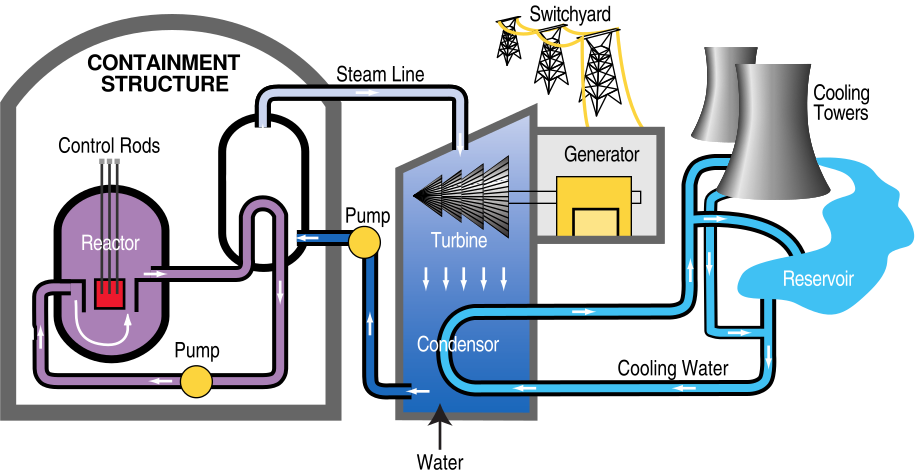
\includegraphics[width=\linewidth,height=0.70\textheight,keepaspectratio]{images-companion/ch01_generation.png}

\caption{Figure C1.1: Pressurized Water Reactor (PWR) Nuclear Power Plant Diagram}

\end{figure}

\begin{figure}[H]

\hypertarget{fig-c1-2}{}\label{fig-c1-2}

\centering

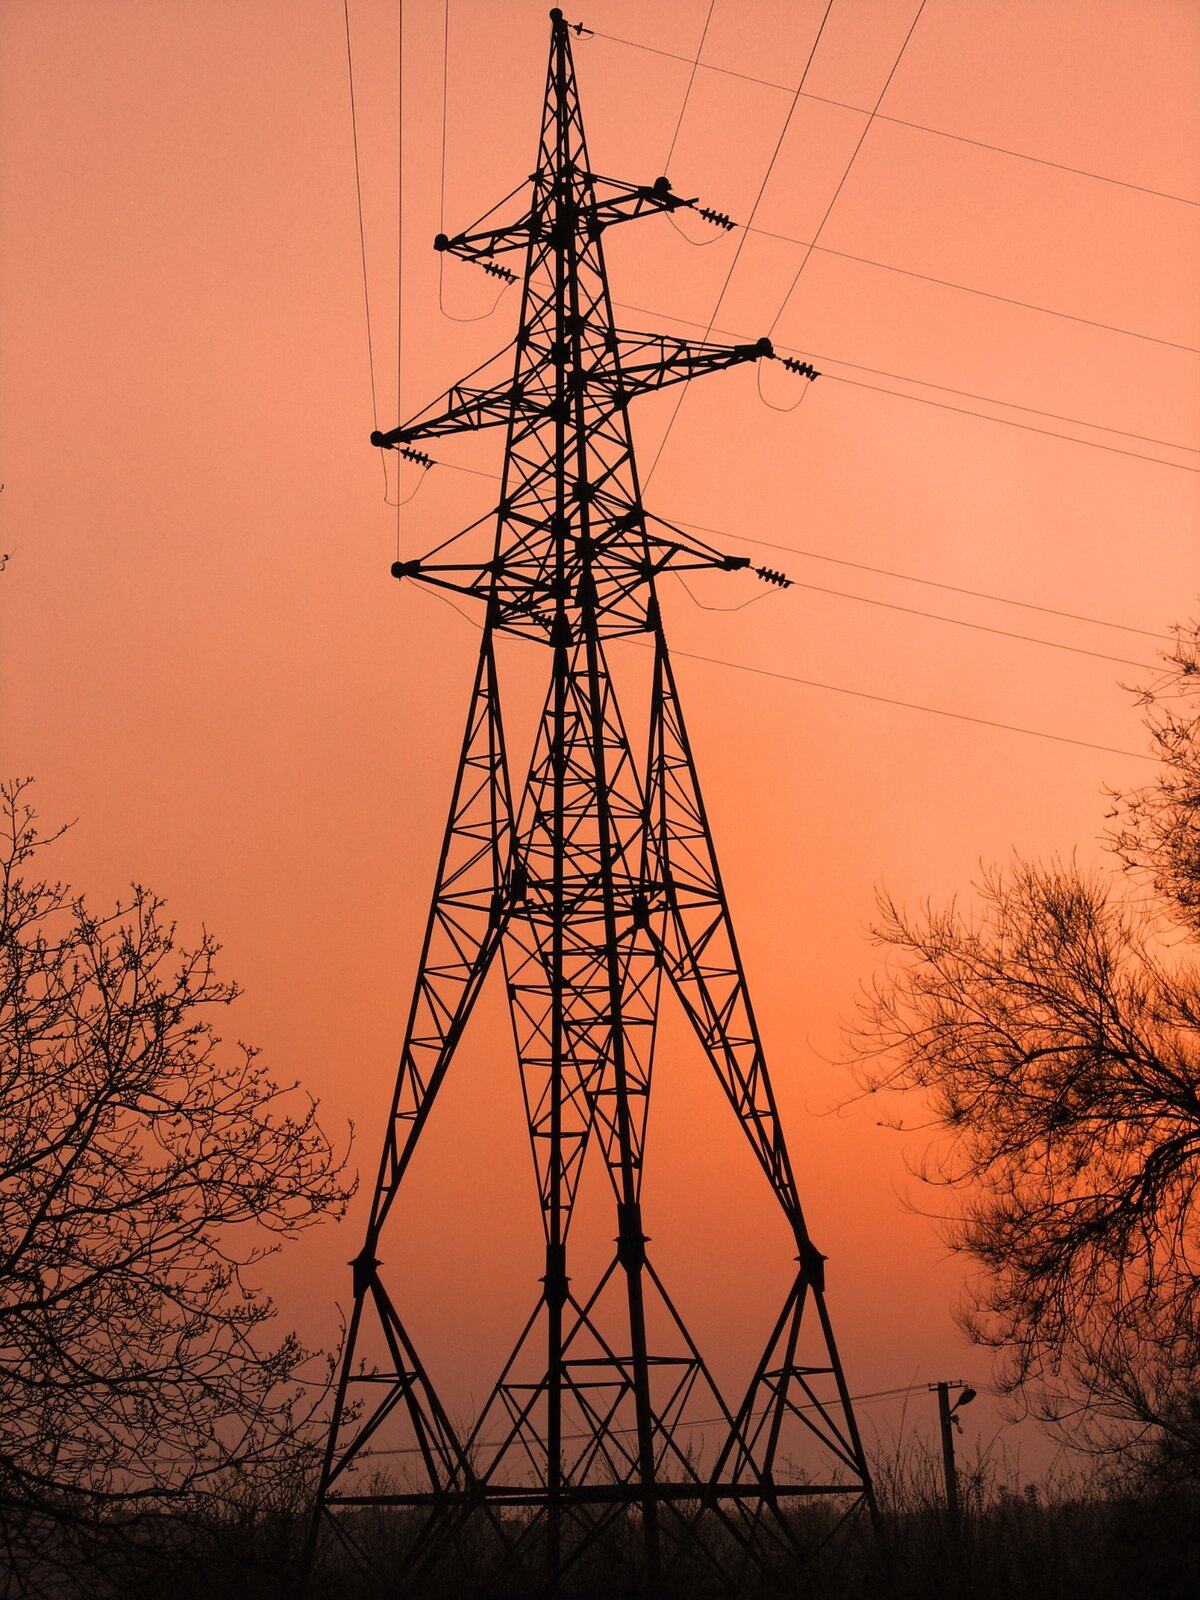
\includegraphics[width=\linewidth,height=0.70\textheight,keepaspectratio]{images-companion/ch01_transmission.jpg}

\caption{Figure C1.2: High-Voltage Transmission Tower}

\end{figure}

\begin{figure}[H]

\hypertarget{fig-c1-3}{}\label{fig-c1-3}

\centering

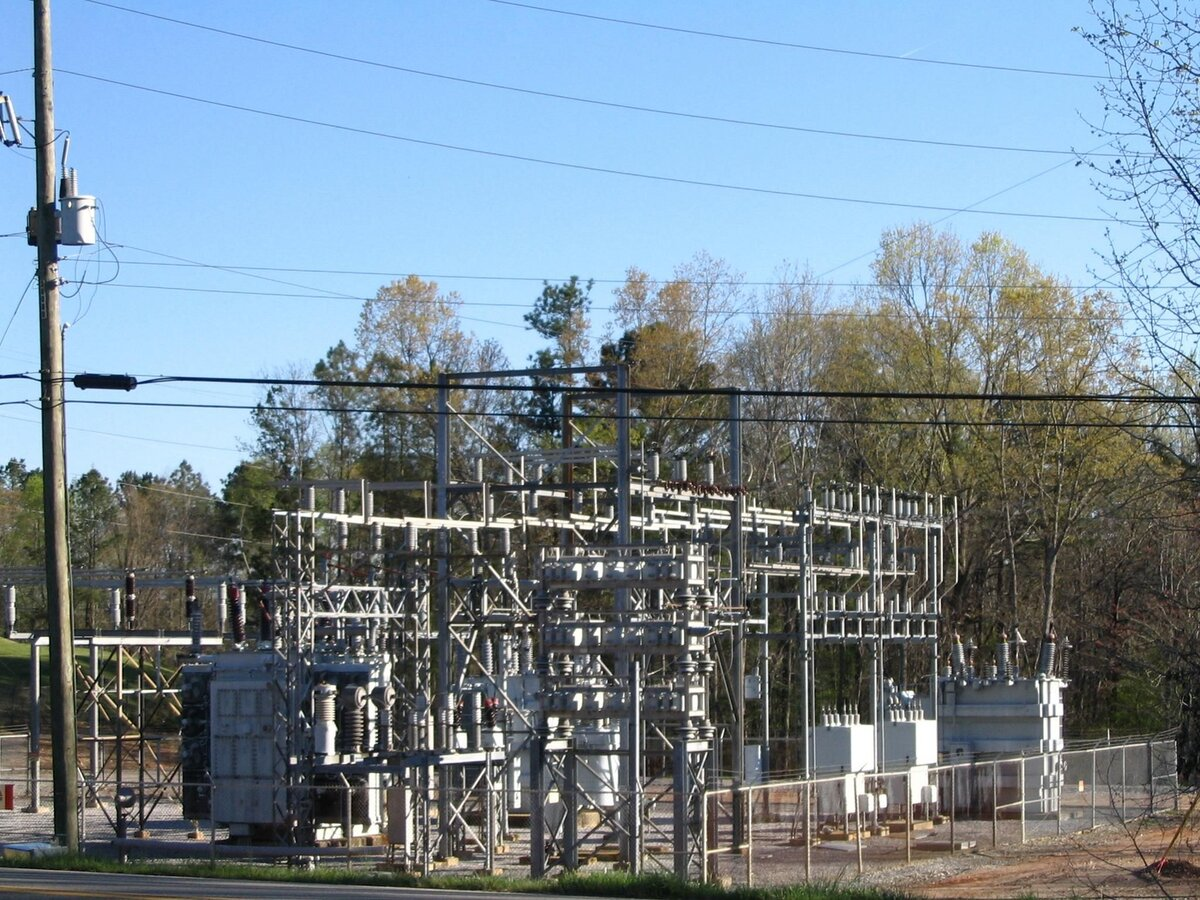
\includegraphics[width=\linewidth,height=0.70\textheight,keepaspectratio]{images-companion/ch01_distribution.jpg}

\caption{Figure C1.3: Outdoor Power Distribution Substation}

\end{figure}

\begin{figure}[H]

\hypertarget{fig-c1-4}{}\label{fig-c1-4}

\centering

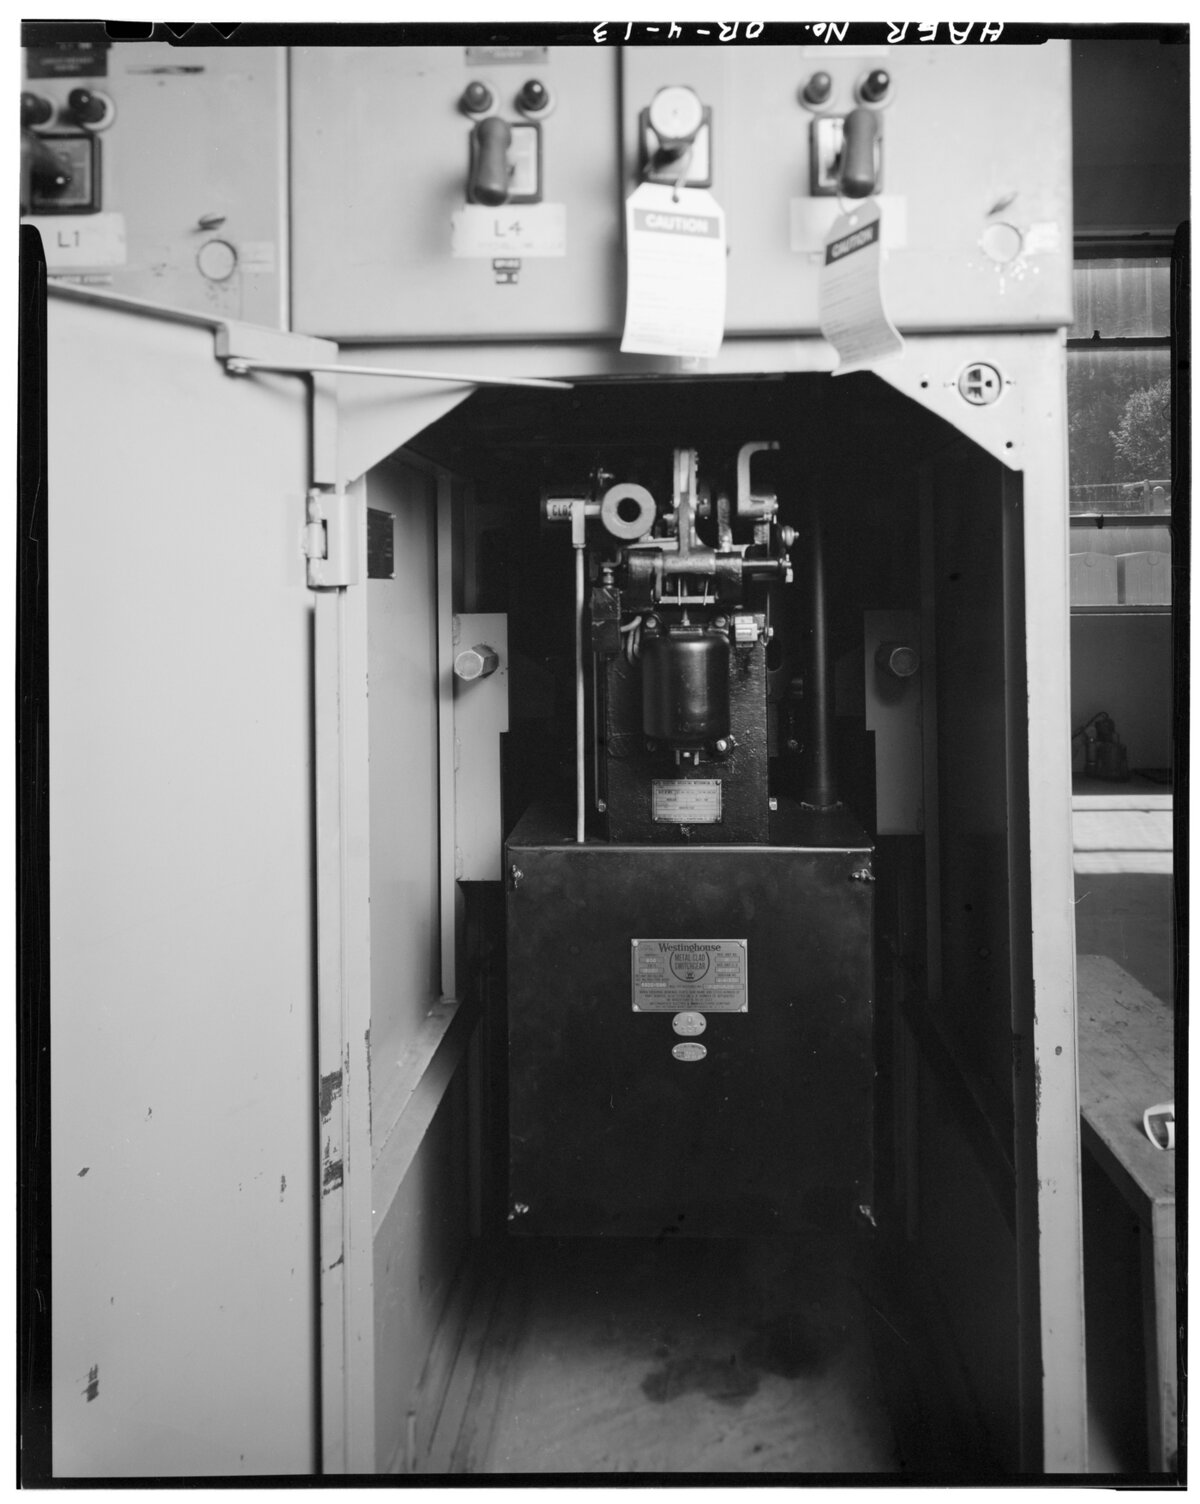
\includegraphics[width=\linewidth,height=0.70\textheight,keepaspectratio]{images-companion/ch01_protection.jpg}

\caption{Figure C1.4: Substation Power Circuit Breaker, Metal-Clad Switchgear}

\end{figure}

\begin{figure}[H]

\hypertarget{fig-c1-5}{}\label{fig-c1-5}

\centering

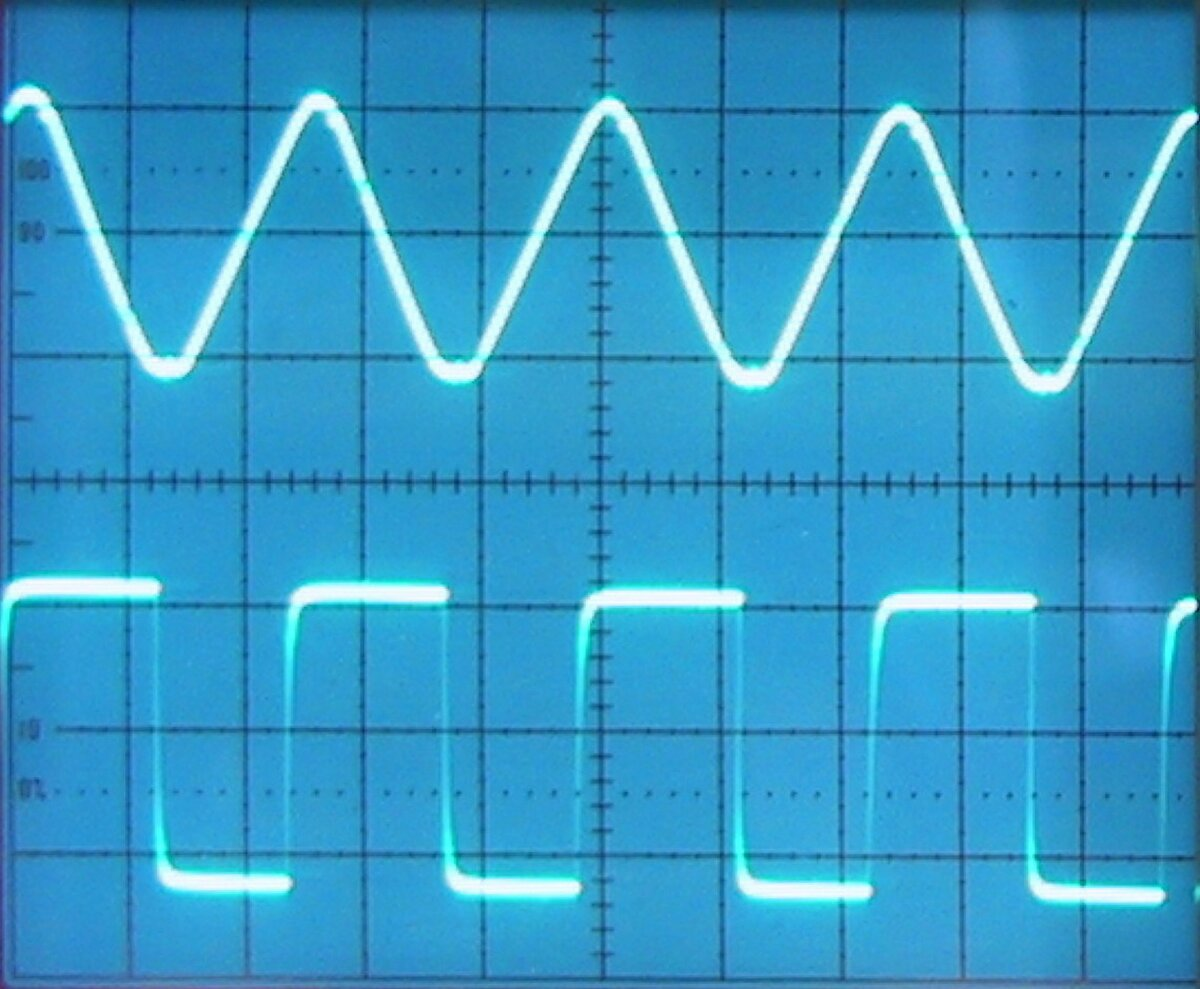
\includegraphics[width=\linewidth,height=0.70\textheight,keepaspectratio]{images-companion/ch01_power_quality.jpg}

\caption{Figure C1.5: Fundamental and Harmonic Waveforms on an Oscilloscope}

\end{figure}

\begin{figure}[H]

\hypertarget{fig-c1-6}{}\label{fig-c1-6}

\centering

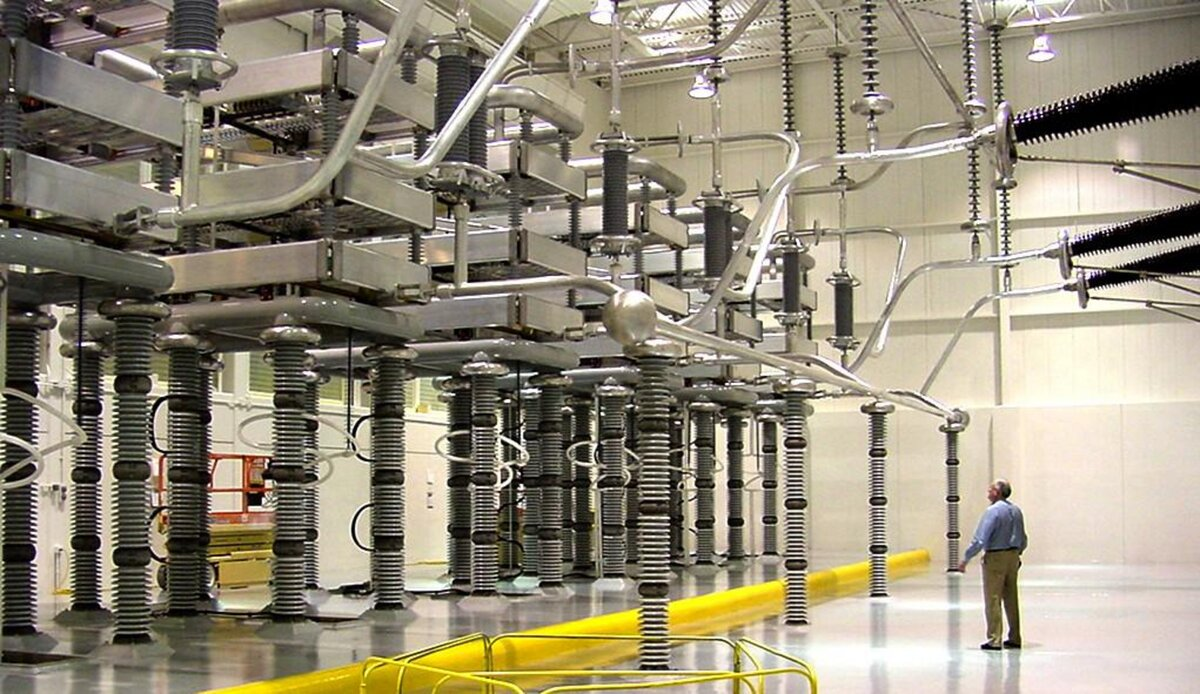
\includegraphics[width=\linewidth,height=0.70\textheight,keepaspectratio]{images-companion/ch01_hvdc.jpg}

\caption{Figure C1.6: Celilo Converter Station, Pacific DC Intertie (HVDC Terminal)}

\end{figure}

\begin{figure}[H]

\hypertarget{fig-c1-7}{}\label{fig-c1-7}

\centering

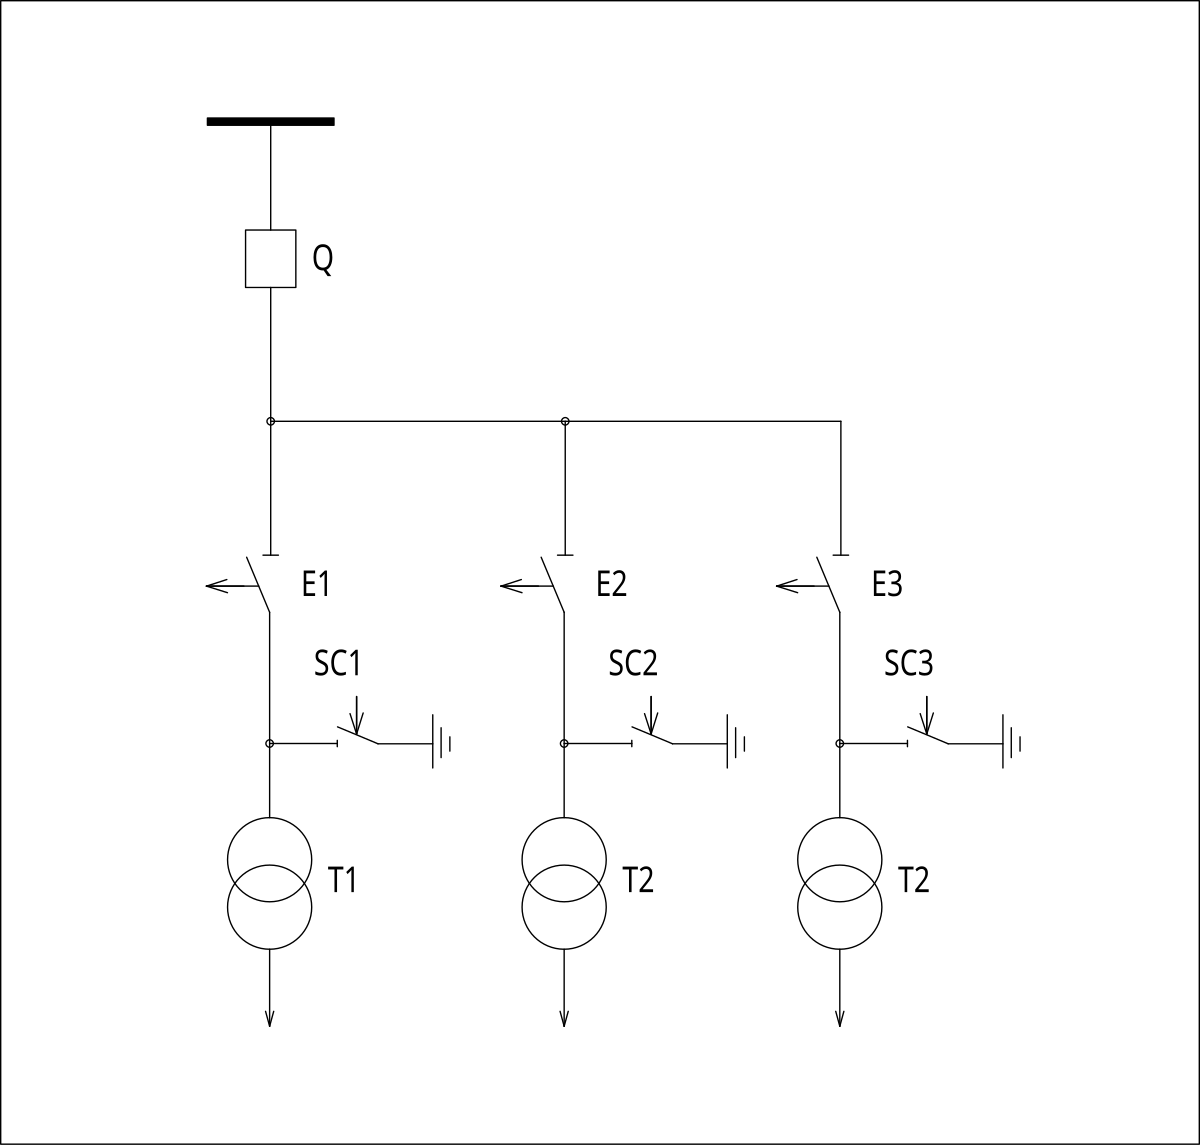
\includegraphics[width=\linewidth,height=0.70\textheight,keepaspectratio]{images-companion/ch01_loadflow.png}

\caption{Figure C1.7: One-Line Diagram of a Distribution Substation}

\end{figure}

\begin{figure}[H]

\hypertarget{fig-c1-8}{}\label{fig-c1-8}

\centering

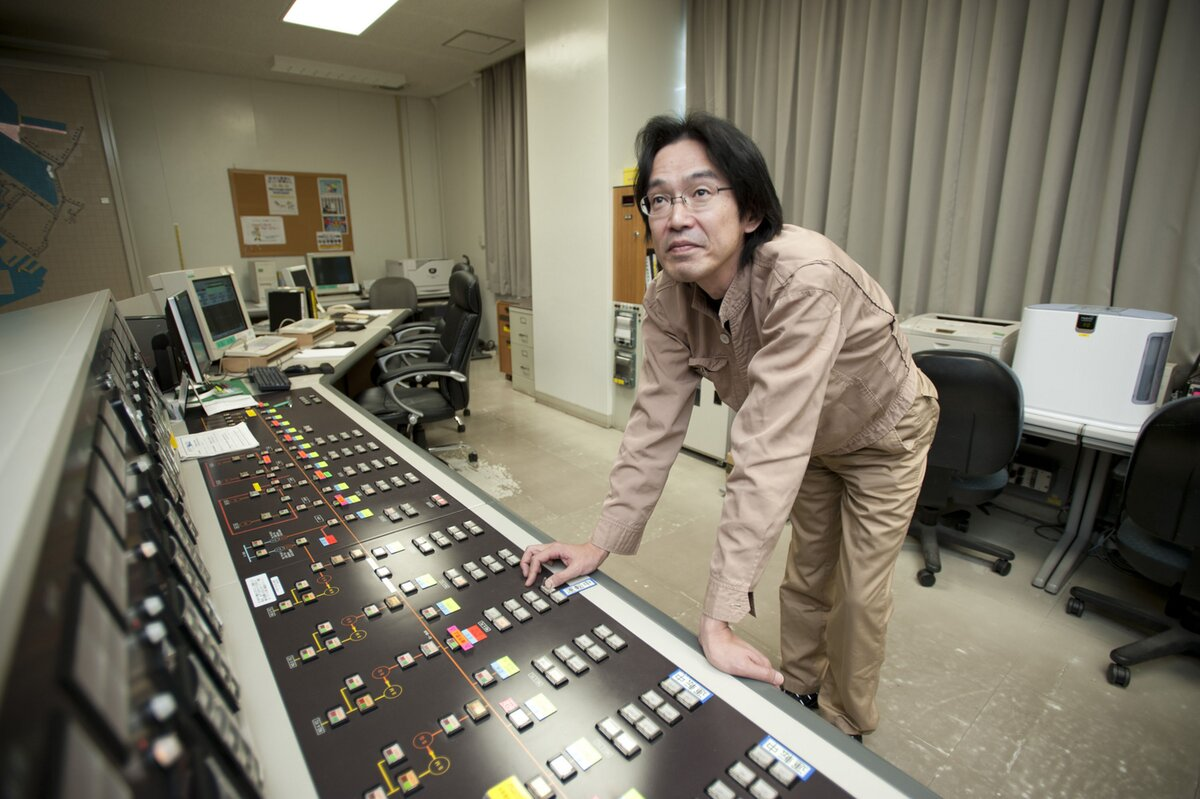
\includegraphics[width=\linewidth,height=0.70\textheight,keepaspectratio]{images-companion/ch01_scada.jpg}

\caption{Figure C1.8: SCADA Operator Balancing Electrical Load}

\end{figure}

\section{Chapter 2: Communications
Engineering}\label{chapter-2-communications-engineering}

\begin{figure}[H]

\hypertarget{fig-c2-1}{}\label{fig-c2-1}

\centering

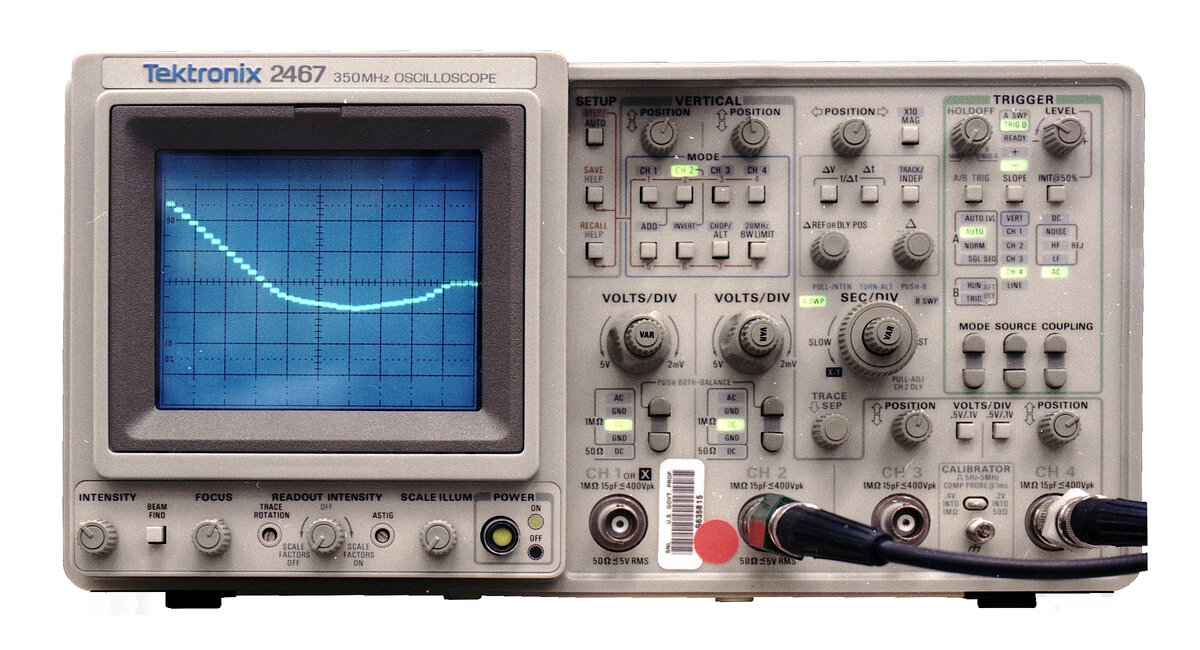
\includegraphics[width=\linewidth,height=0.70\textheight,keepaspectratio]{images-companion/ch02_analog.jpg}

\caption{Figure C2.1: Analog Oscilloscope for Analog Signal Observation}

\end{figure}

\begin{figure}[H]

\hypertarget{fig-c2-2}{}\label{fig-c2-2}

\centering

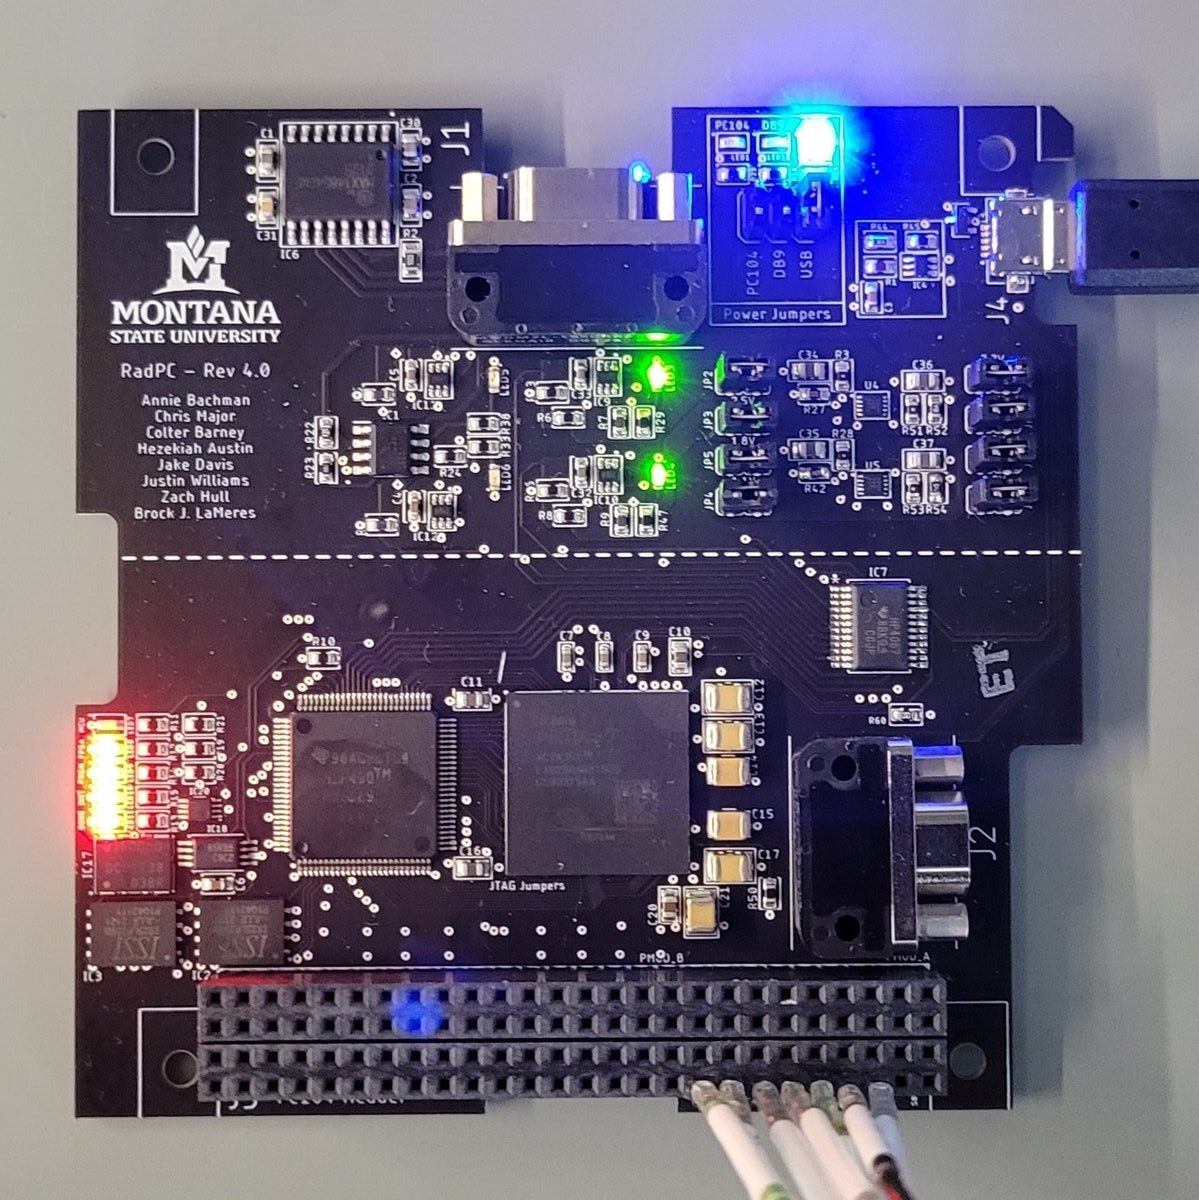
\includegraphics[width=\linewidth,height=0.70\textheight,keepaspectratio]{images-companion/ch02_dsp.jpg}

\caption{Figure C2.2: FPGA-Based Digital Signal Processing Board}

\end{figure}

\begin{figure}[H]

\hypertarget{fig-c2-3}{}\label{fig-c2-3}

\centering

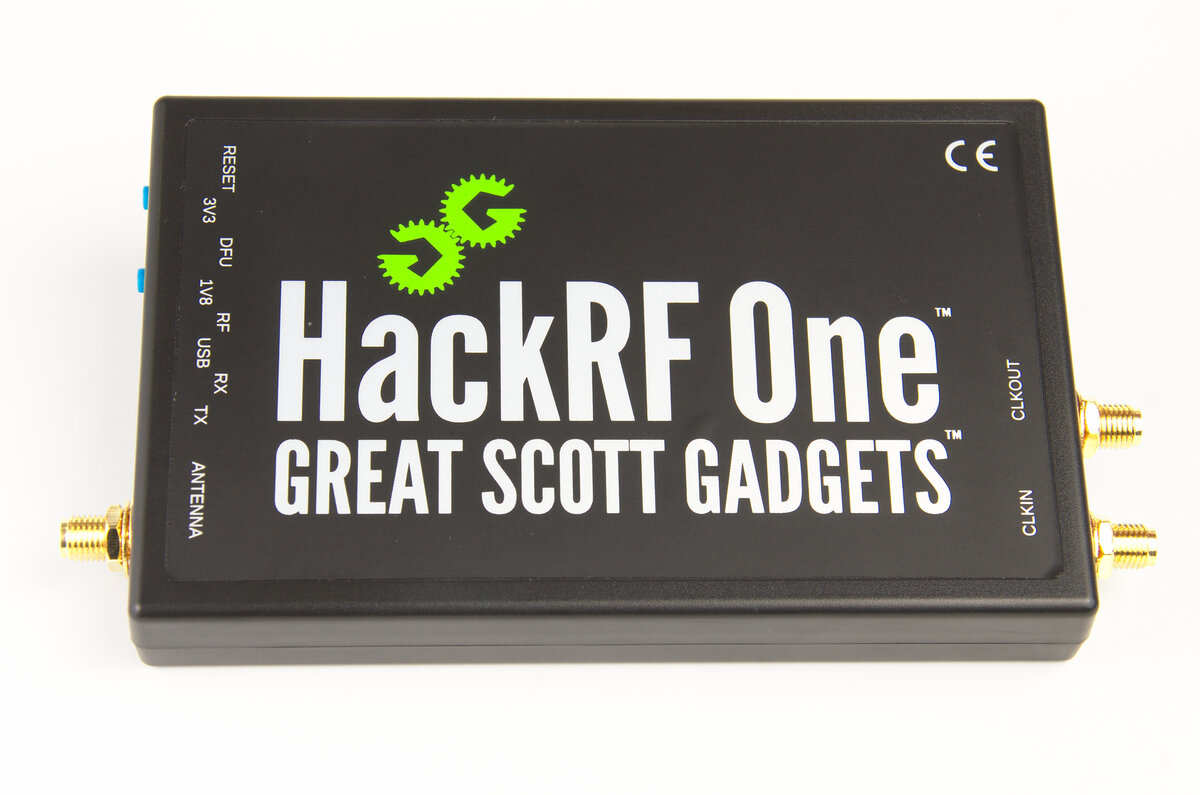
\includegraphics[width=\linewidth,height=0.70\textheight,keepaspectratio]{images-companion/ch02_modulation.jpg}

\caption{Figure C2.3: HackRF One Software-Defined Radio Transceiver}

\end{figure}

\begin{figure}[H]

\hypertarget{fig-c2-4}{}\label{fig-c2-4}

\centering

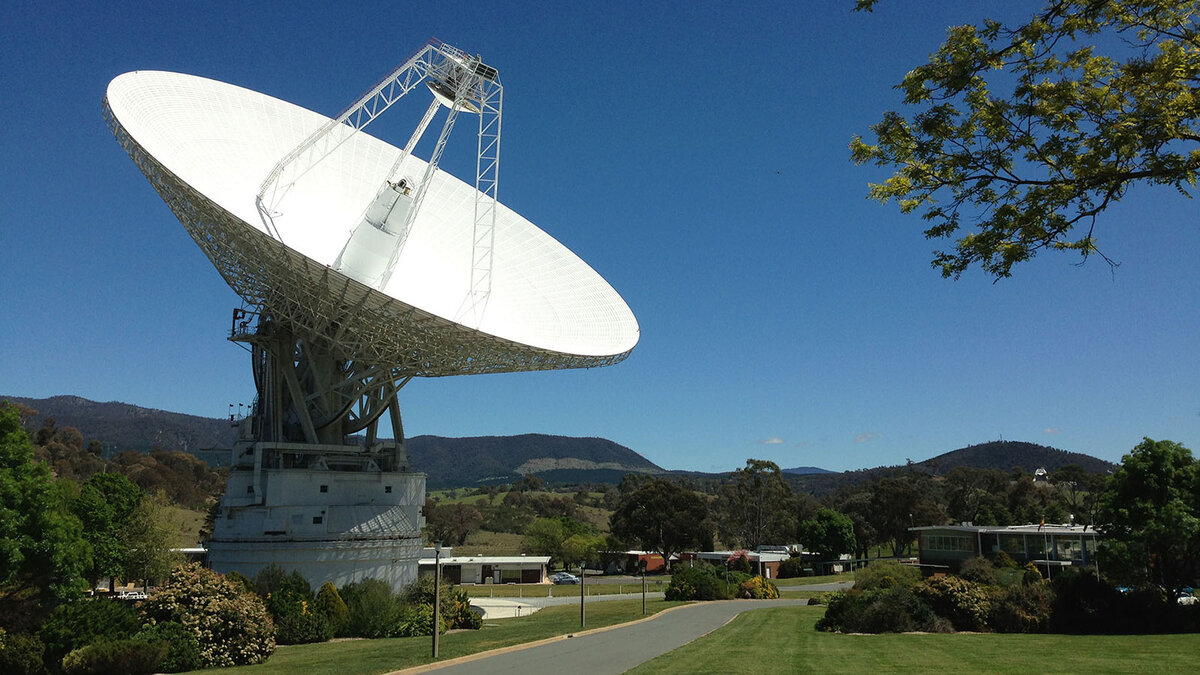
\includegraphics[width=\linewidth,height=0.70\textheight,keepaspectratio]{images-companion/ch02_coding.jpg}

\caption{Figure C2.4: DSN Deep-Space Antenna (Canberra) — Channel Coding Heritage from Deep-Space Links}

\end{figure}

\begin{figure}[H]

\hypertarget{fig-c2-5}{}\label{fig-c2-5}

\centering

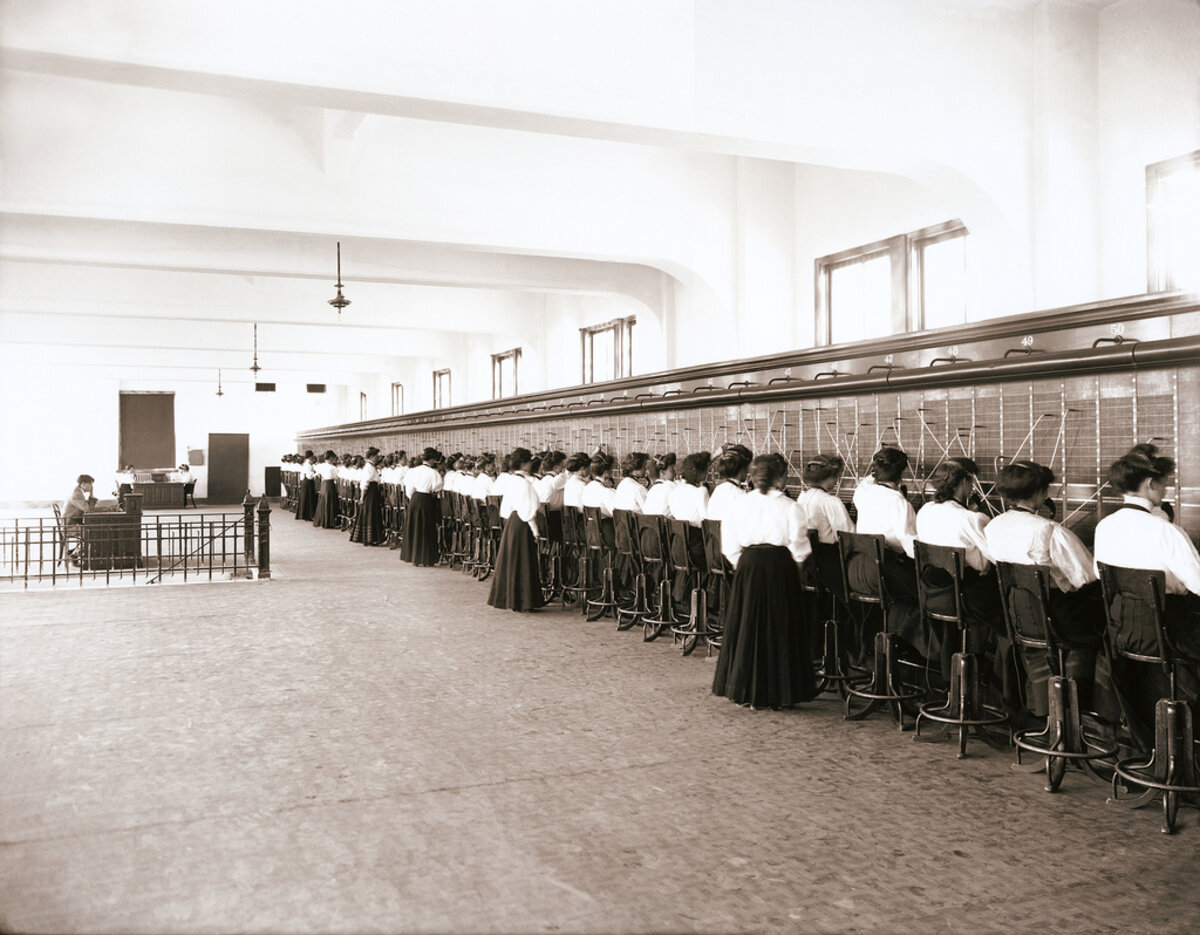
\includegraphics[width=\linewidth,height=0.70\textheight,keepaspectratio]{images-companion/ch02_muxing.jpg}

\caption{Figure C2.5: Manual Telephone Switchboard, Salt Lake City, 1907}

\end{figure}

\begin{figure}[H]

\hypertarget{fig-c2-6}{}\label{fig-c2-6}

\centering

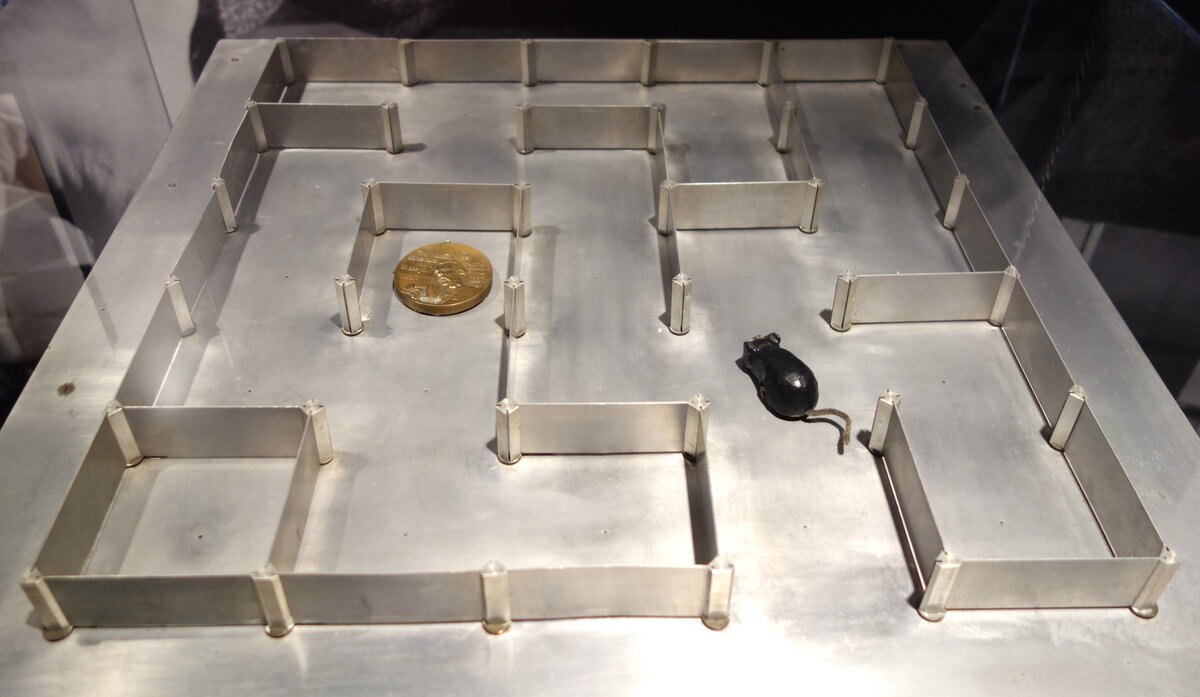
\includegraphics[width=\linewidth,height=0.70\textheight,keepaspectratio]{images-companion/ch02_infotheory.jpg}

\caption{Figure C2.6: Theseus, Claude Shannon’s Maze-Solving Mouse (1952)}

\end{figure}

\begin{figure}[H]

\hypertarget{fig-c2-7}{}\label{fig-c2-7}

\centering

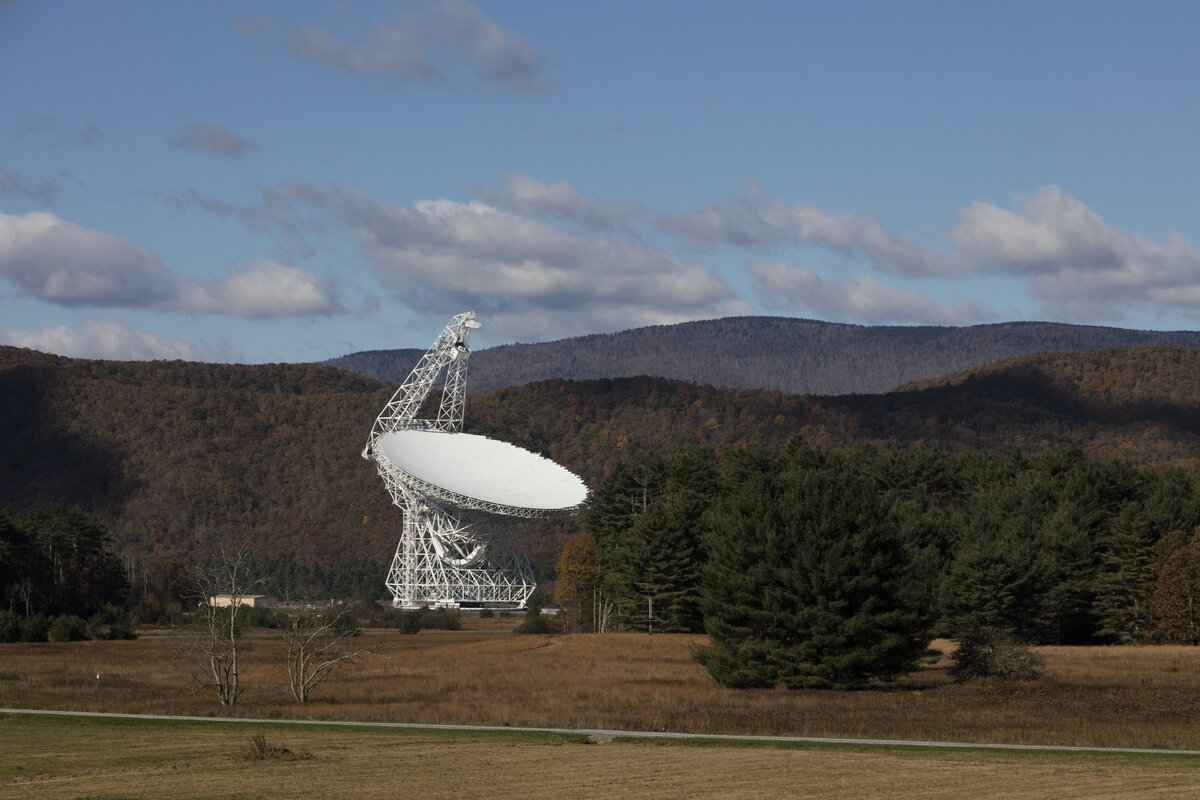
\includegraphics[width=\linewidth,height=0.70\textheight,keepaspectratio]{images-companion/ch02_noise.jpg}

\caption{Figure C2.7: Green Bank Radio Telescope — Low-Noise Receiver Systems}

\end{figure}

\begin{figure}[H]

\hypertarget{fig-c2-8}{}\label{fig-c2-8}

\centering

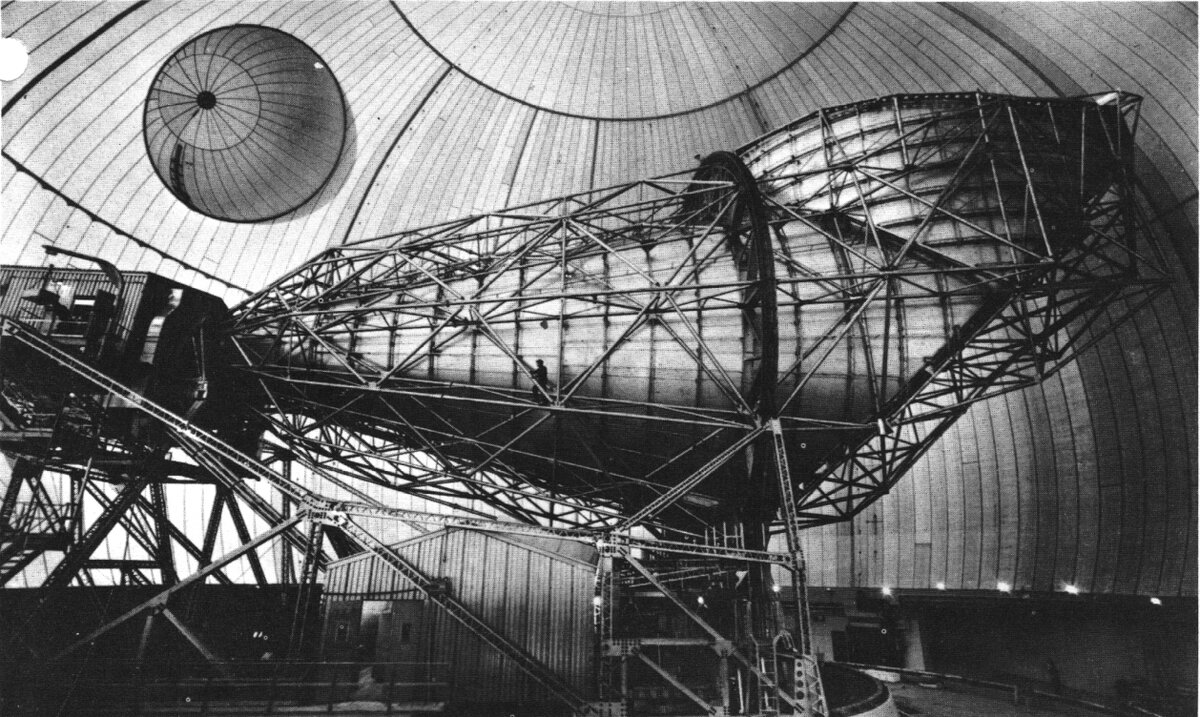
\includegraphics[width=\linewidth,height=0.70\textheight,keepaspectratio]{images-companion/ch02_linkbudget.jpg}

\caption{Figure C2.8: Relay 1 Ground Station Antenna — Early Satellite Communications Link Budget}

\end{figure}

\section{Chapter 3: Semiconductors}\label{chapter-3-semiconductors}

\begin{figure}[H]

\hypertarget{fig-c3-1}{}\label{fig-c3-1}

\centering

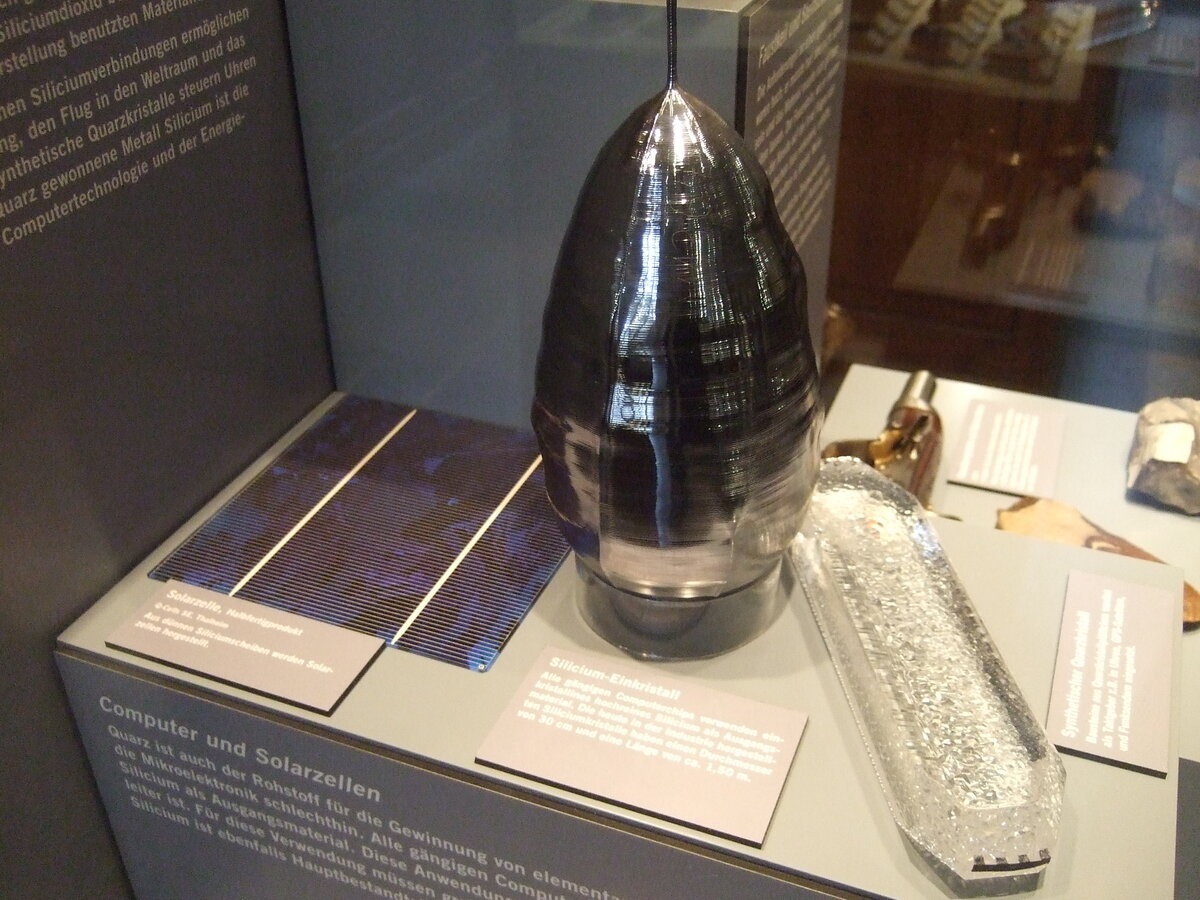
\includegraphics[width=\linewidth,height=0.70\textheight,keepaspectratio]{images-companion/ch03_fundamentals.jpg}

\caption{Figure C3.1: Single-Crystal Silicon Boule and Wafer}

\end{figure}

\begin{figure}[H]

\hypertarget{fig-c3-2}{}\label{fig-c3-2}

\centering

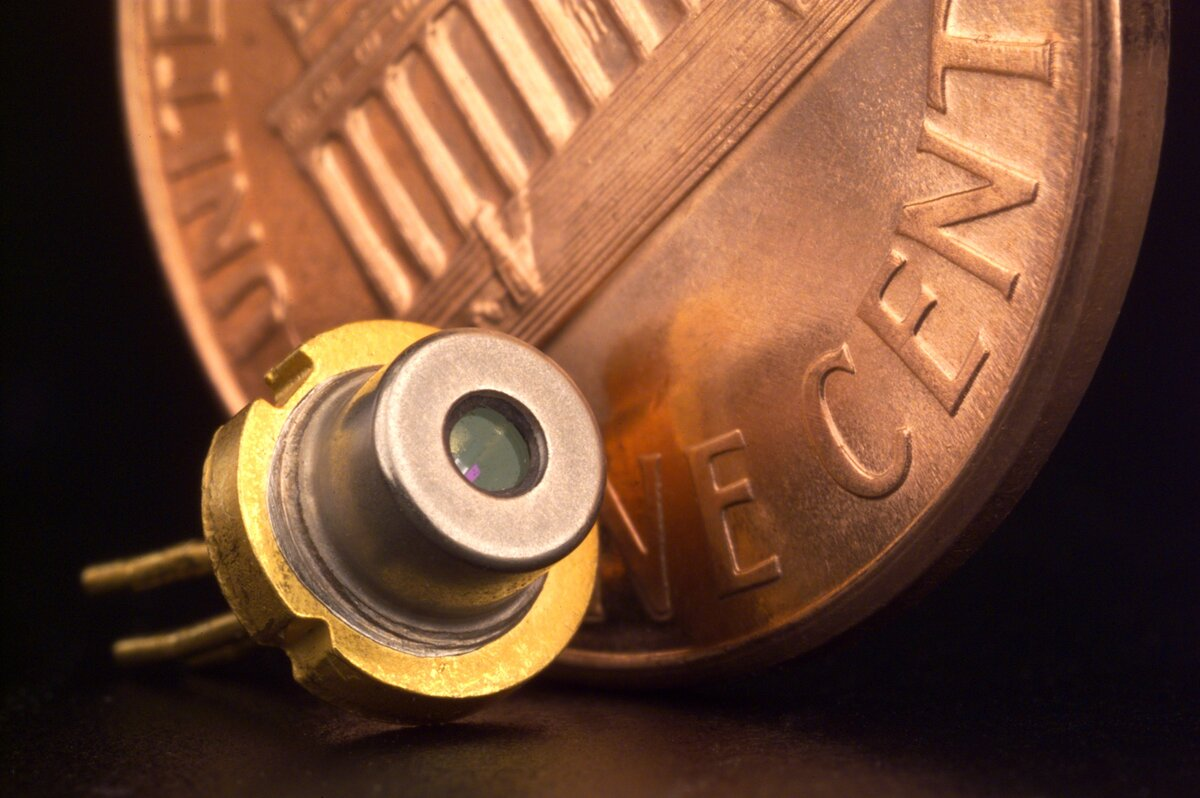
\includegraphics[width=\linewidth,height=0.70\textheight,keepaspectratio]{images-companion/ch03_materials.jpg}

\caption{Figure C3.2: Compound-Semiconductor Laser Diode Die (Shown Against a Penny for Scale)}

\end{figure}

\begin{figure}[H]

\hypertarget{fig-c3-3}{}\label{fig-c3-3}

\centering

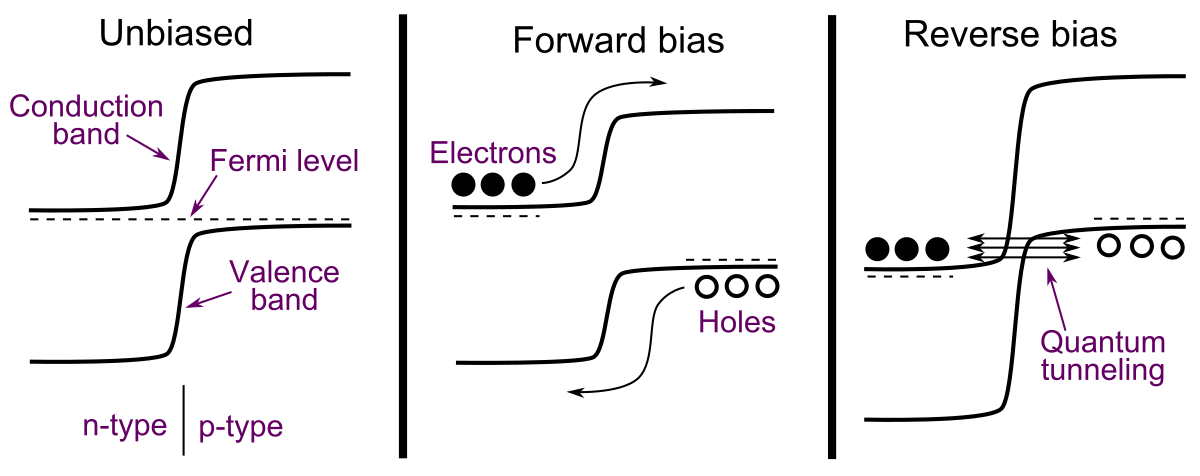
\includegraphics[width=\linewidth,height=0.70\textheight,keepaspectratio]{images-companion/ch03_pnjunction.png}

\caption{Figure C3.3: Energy-Band Diagram of a PN Junction — Unbiased, Forward-Bias, and Reverse-Bias Conditions}

\end{figure}

\begin{figure}[H]

\hypertarget{fig-c3-4}{}\label{fig-c3-4}

\centering

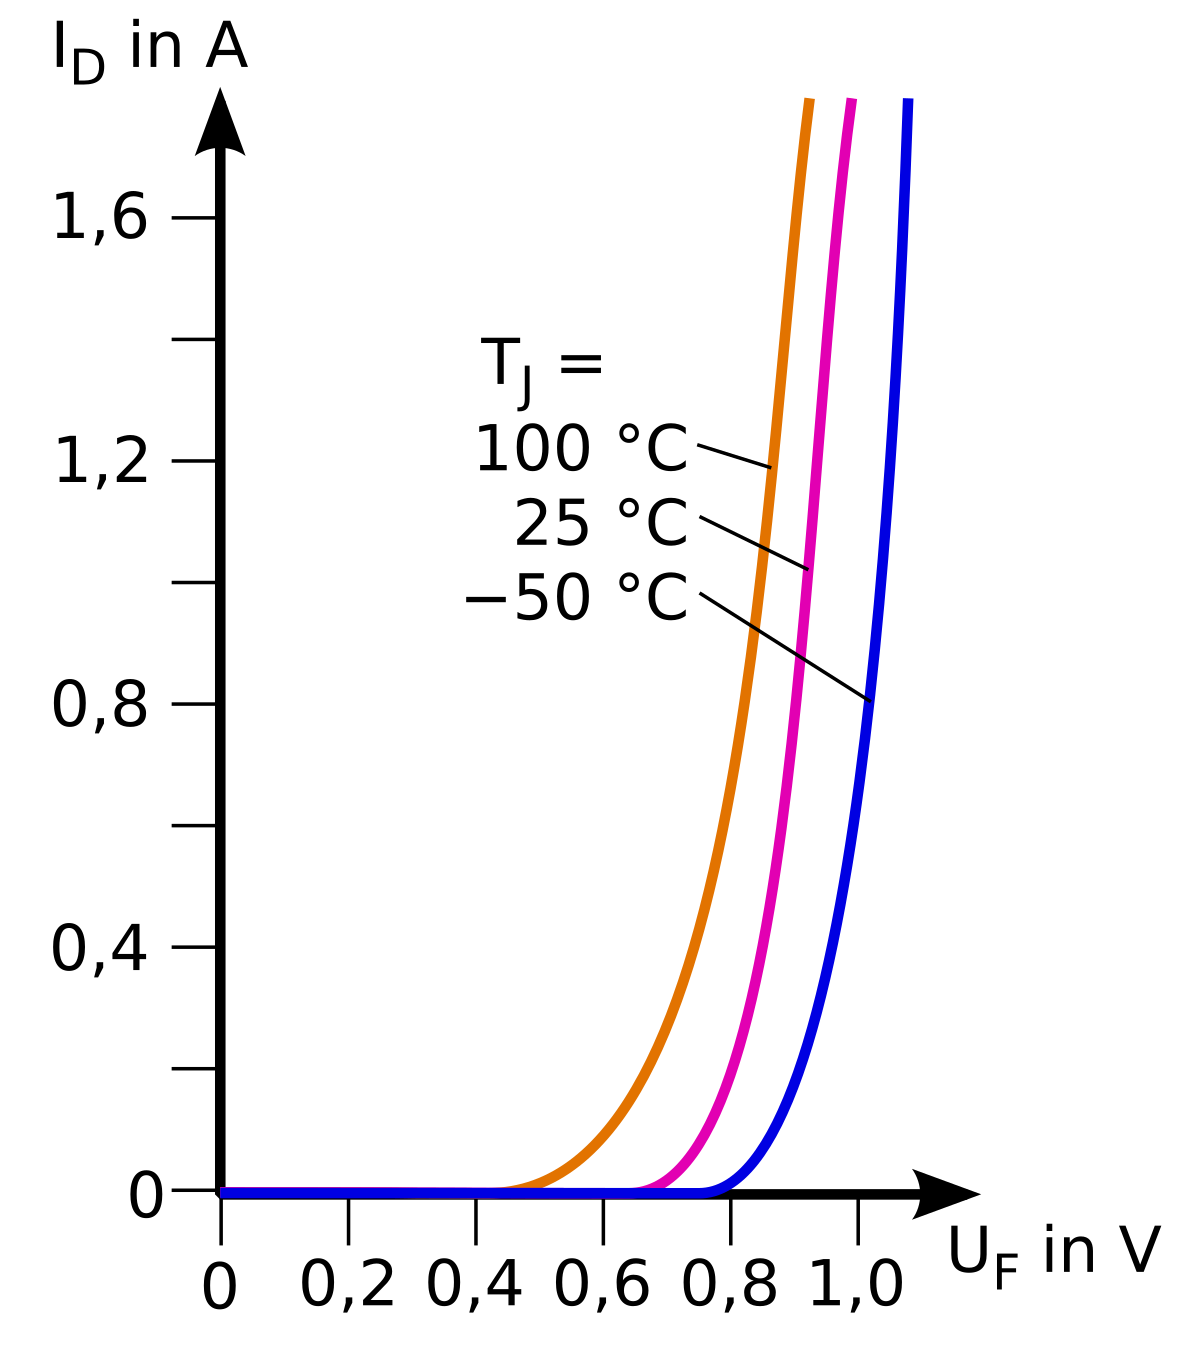
\includegraphics[width=\linewidth,height=0.70\textheight,keepaspectratio]{images-companion/ch03_diodes.png}

\caption{Figure C3.4: Measured I-V Characteristic Curve of a 1N4001 Diode}

\end{figure}

\begin{figure}[H]

\hypertarget{fig-c3-5}{}\label{fig-c3-5}

\centering

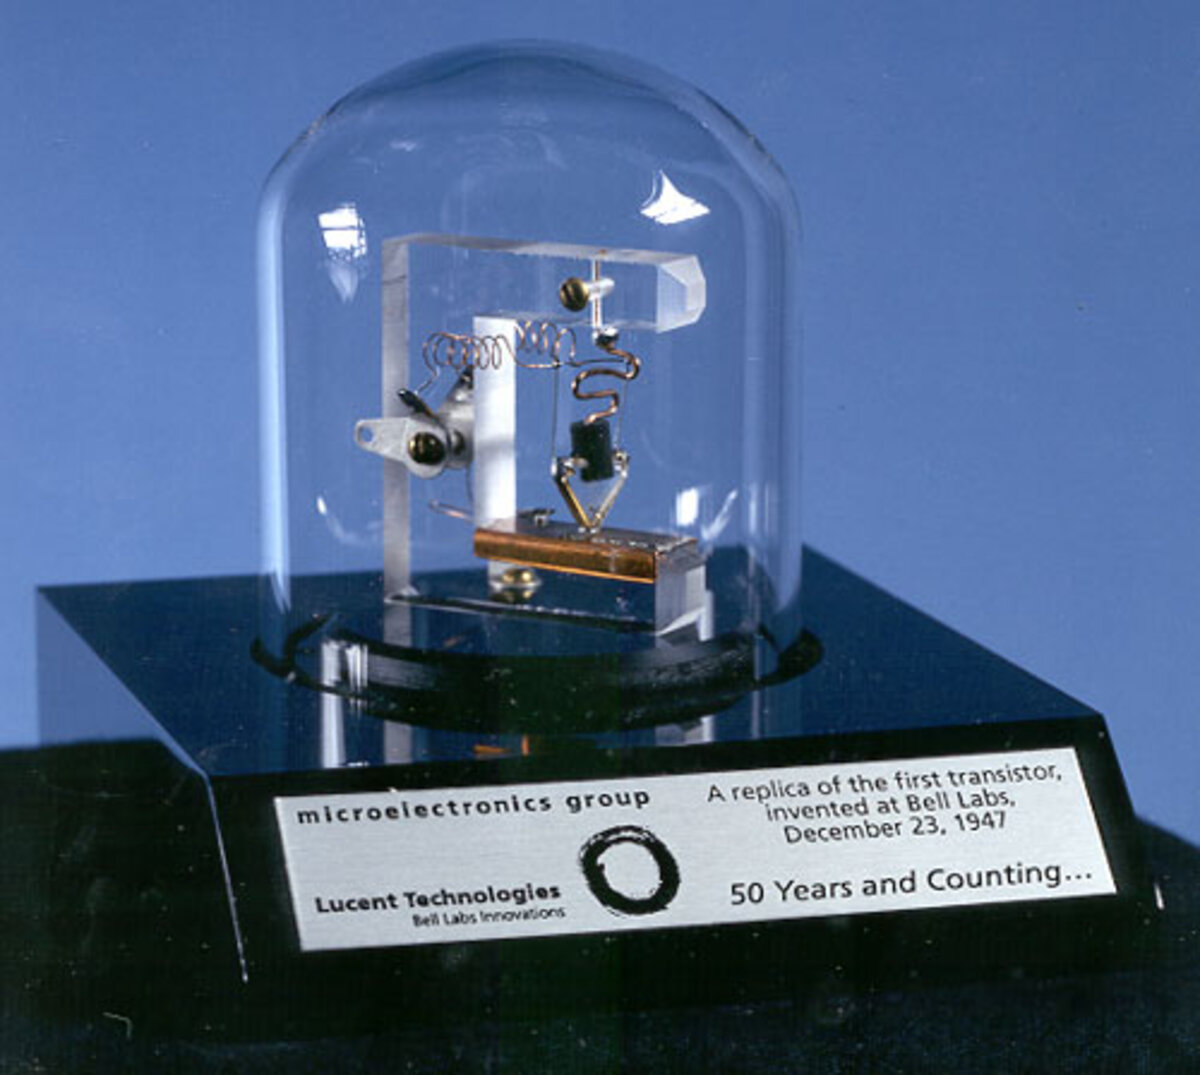
\includegraphics[width=\linewidth,height=0.70\textheight,keepaspectratio]{images-companion/ch03_transistors.jpg}

\caption{Figure C3.5: Replica of the First Point-Contact Transistor (Bell Labs, 1947)}

\end{figure}

\begin{figure}[H]

\hypertarget{fig-c3-6}{}\label{fig-c3-6}

\centering

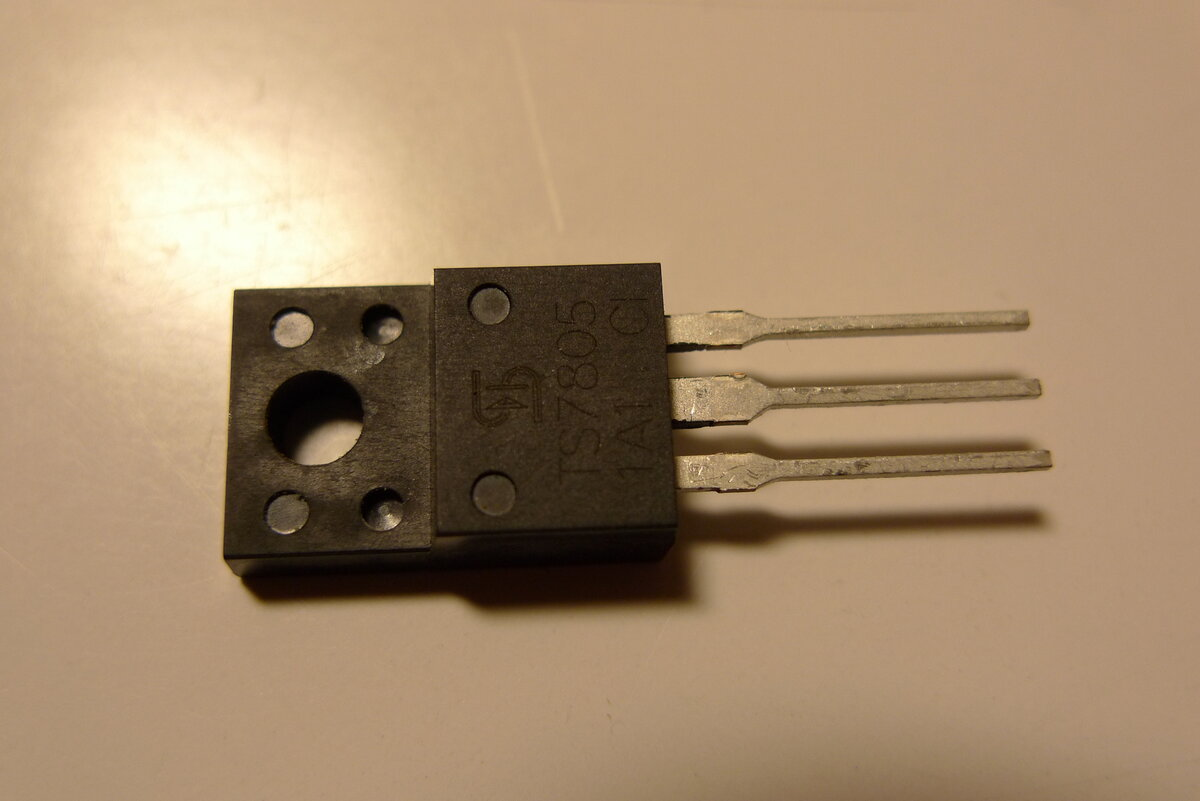
\includegraphics[width=\linewidth,height=0.70\textheight,keepaspectratio]{images-companion/ch03_regulators.jpg}

\caption{Figure C3.6: TS7805 Linear Voltage Regulator in a TO-220 Package}

\end{figure}

\begin{figure}[H]

\hypertarget{fig-c3-7}{}\label{fig-c3-7}

\centering

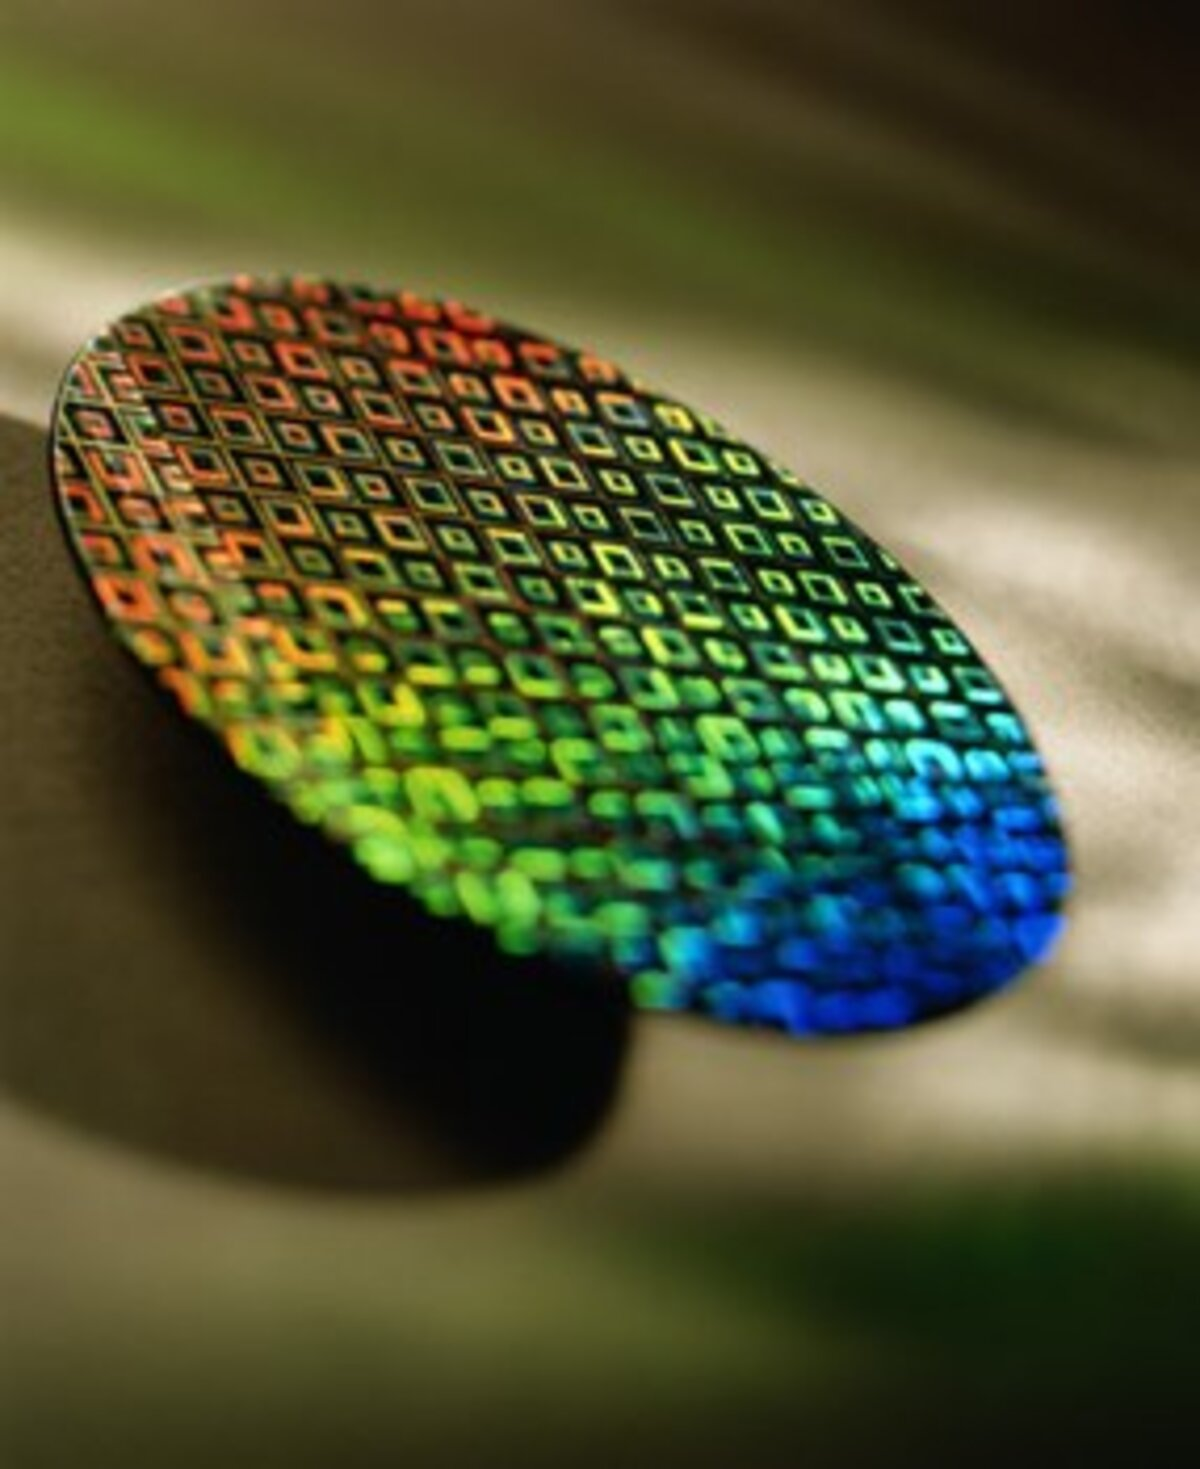
\includegraphics[width=\linewidth,height=0.70\textheight,keepaspectratio]{images-companion/ch03_fabrication.jpg}

\caption{Figure C3.7: Etched Silicon Wafer Showing Individual Die}

\end{figure}

\section{Chapter 4: Control Systems}\label{chapter-4-control-systems}

\begin{figure}[H]

\hypertarget{fig-c4-1}{}\label{fig-c4-1}

\centering

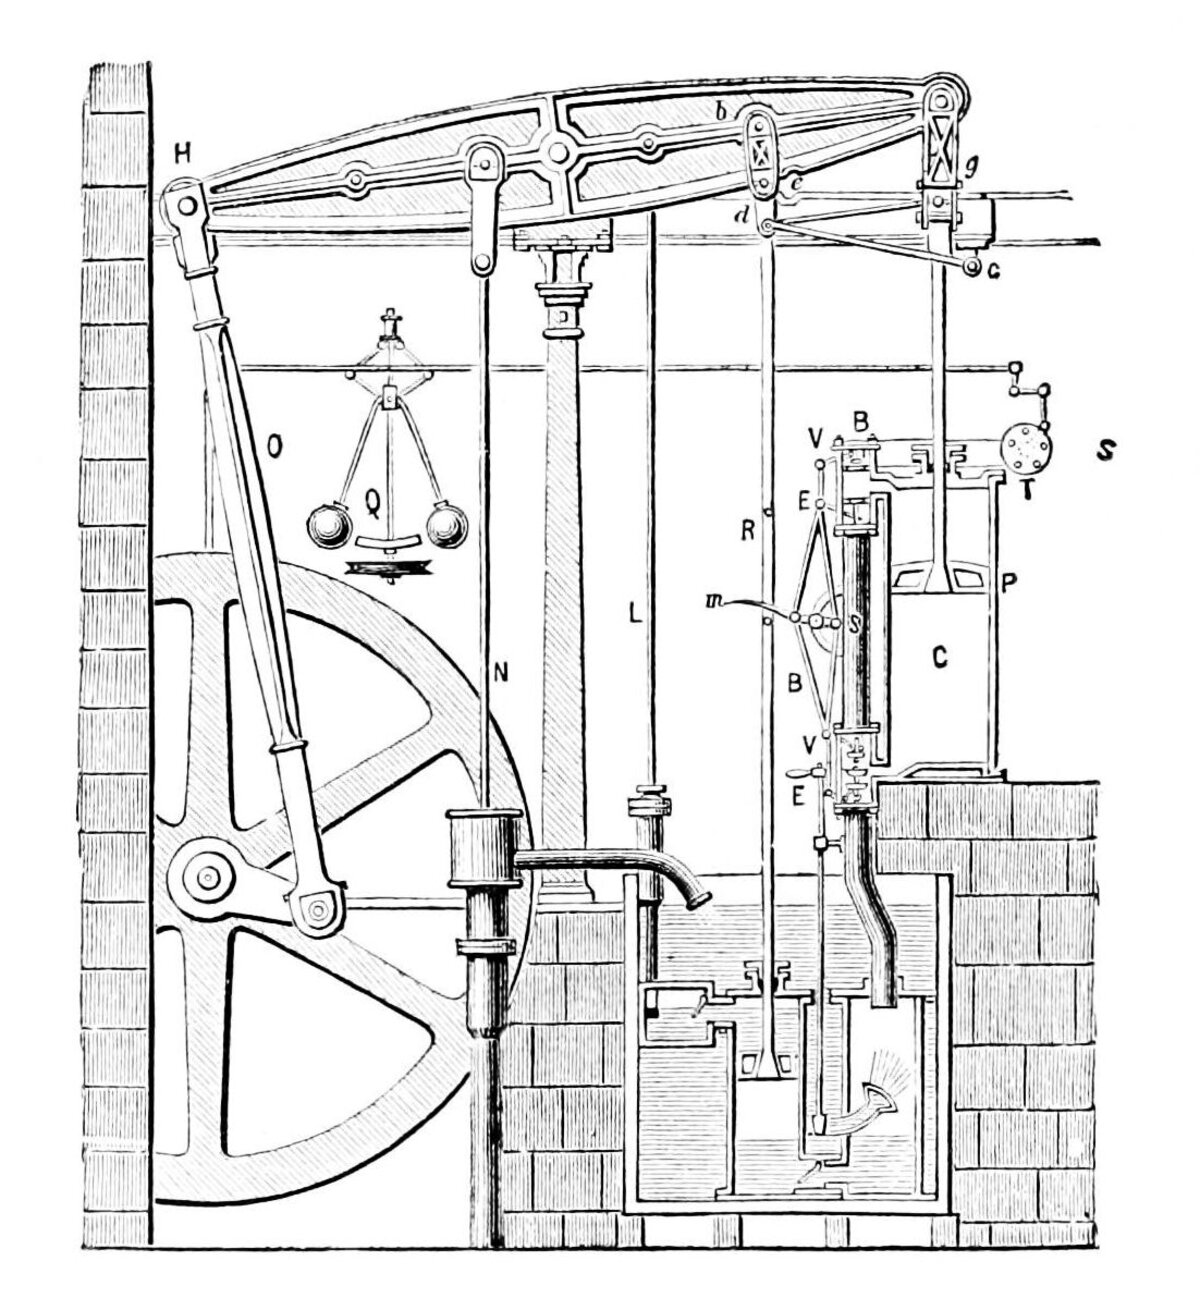
\includegraphics[width=\linewidth,height=0.70\textheight,keepaspectratio]{images-companion/ch04_openloop.jpg}

\caption{Figure C4.1: Watt Steam Engine (1780) — Uncontrolled (Open-Loop) Mechanism}

\end{figure}

\begin{figure}[H]

\hypertarget{fig-c4-2}{}\label{fig-c4-2}

\centering

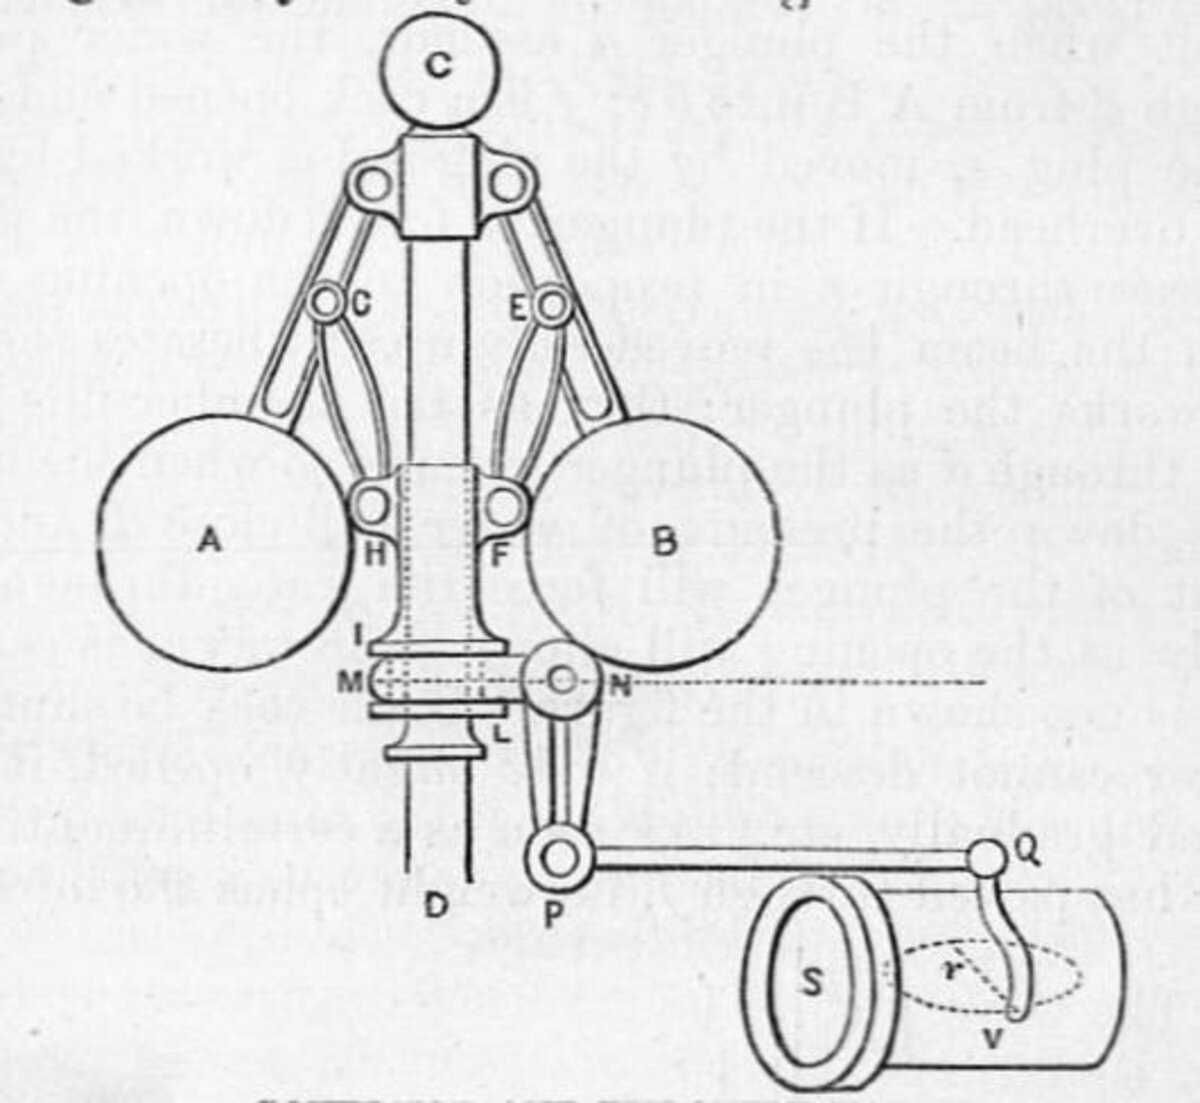
\includegraphics[width=\linewidth,height=0.70\textheight,keepaspectratio]{images-companion/ch04_closedloop.jpg}

\caption{Figure C4.2: Watt’s Centrifugal Flyball Governor — the First Widely Used Closed-Loop Feedback Controller}

\end{figure}

\begin{figure}[H]

\hypertarget{fig-c4-3}{}\label{fig-c4-3}

\centering

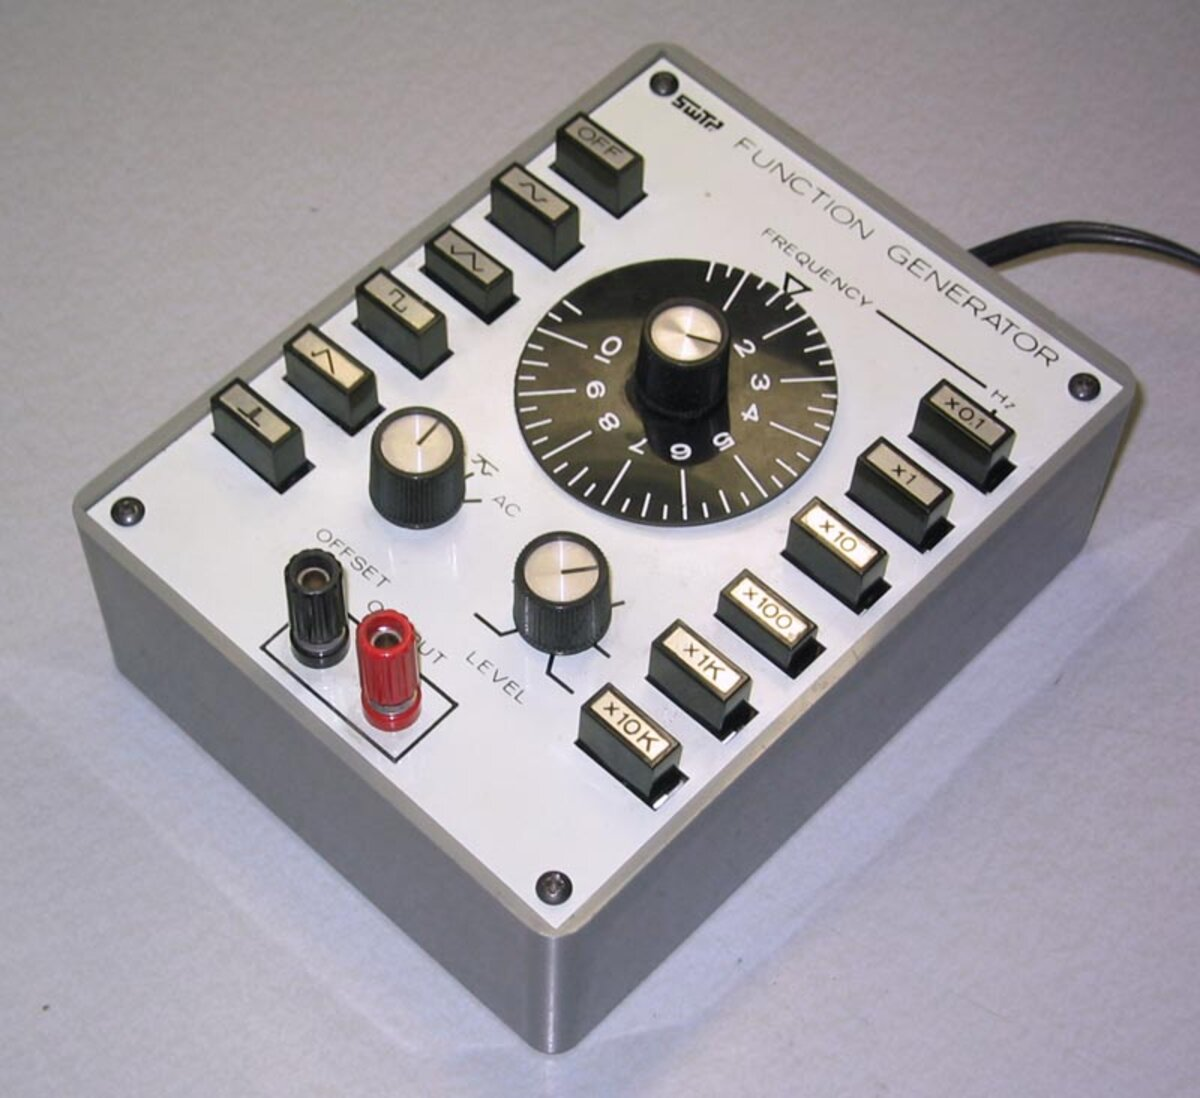
\includegraphics[width=\linewidth,height=0.70\textheight,keepaspectratio]{images-companion/ch04_controlsignals.jpg}

\caption{Figure C4.3: Function Generator for Producing Reference Control Signals}

\end{figure}

\begin{figure}[H]

\hypertarget{fig-c4-4}{}\label{fig-c4-4}

\centering

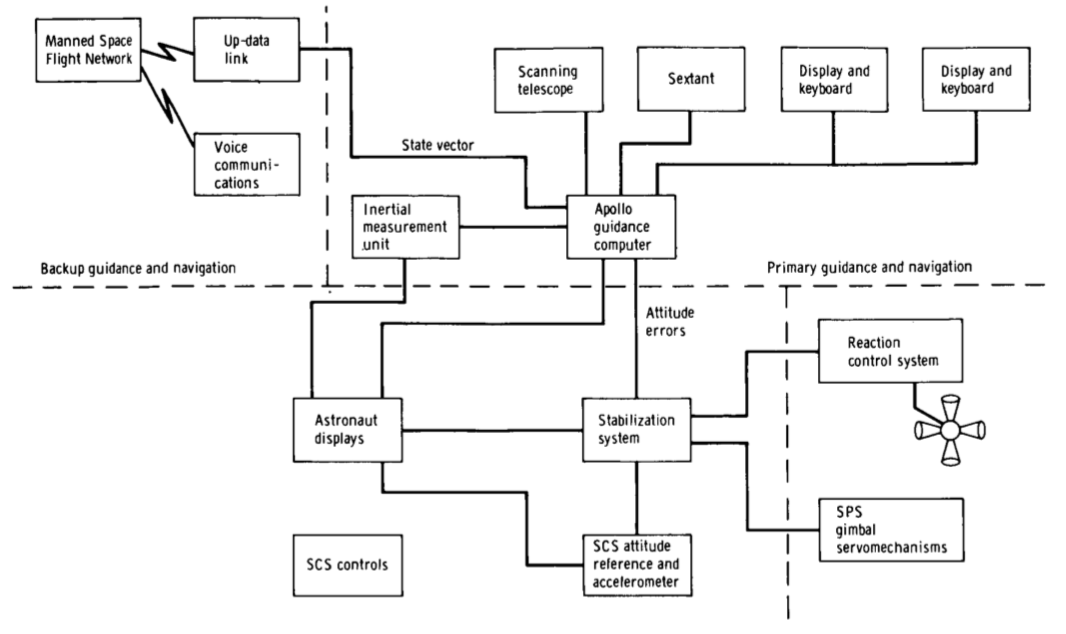
\includegraphics[width=\linewidth,height=0.70\textheight,keepaspectratio]{images-companion/ch04_blockdiagram.png}

\caption{Figure C4.4: Apollo Block I Guidance System Block Diagram}

\end{figure}

\begin{figure}[H]

\hypertarget{fig-c4-5}{}\label{fig-c4-5}

\centering

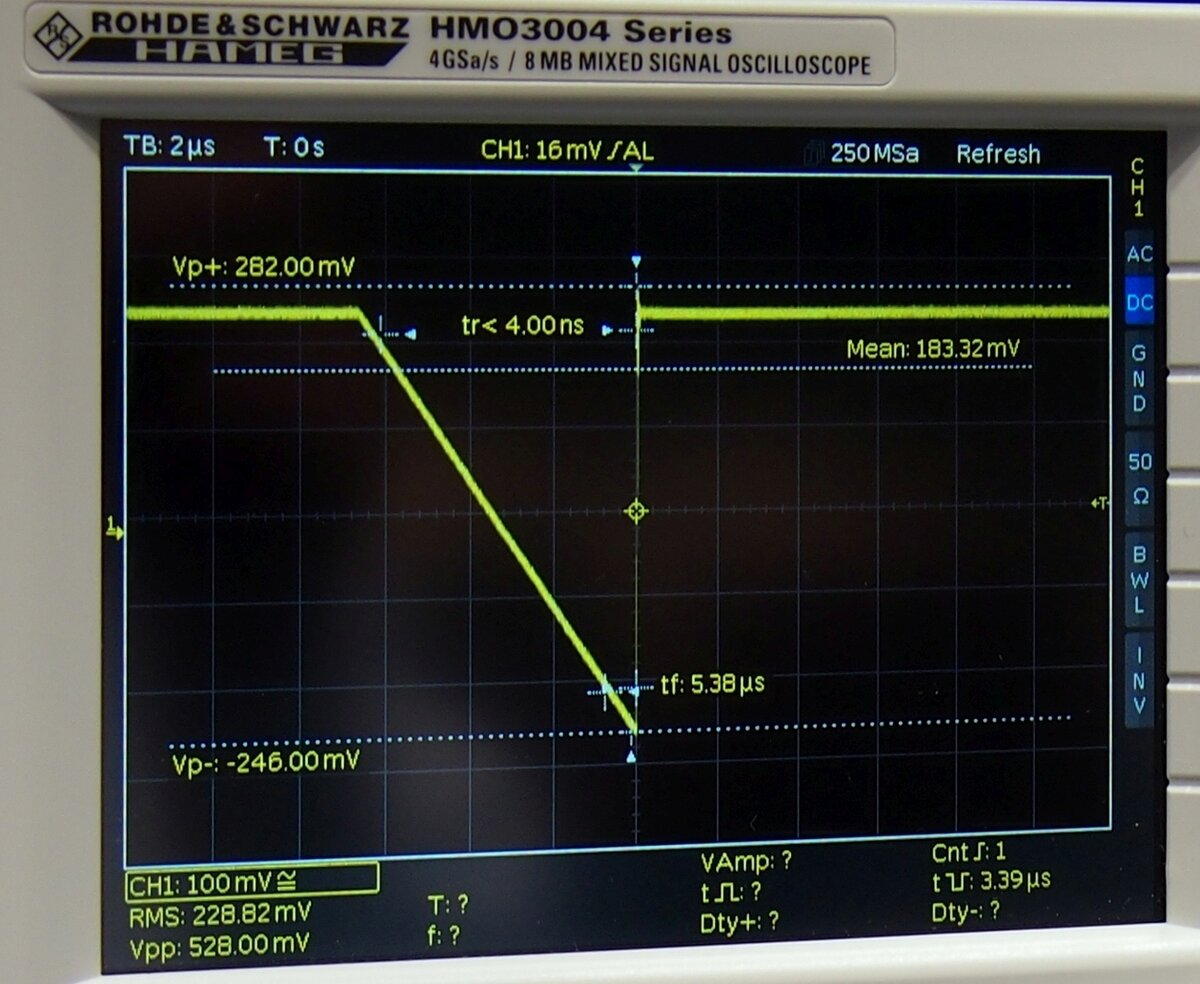
\includegraphics[width=\linewidth,height=0.70\textheight,keepaspectratio]{images-companion/ch04_timedomain.jpg}

\caption{Figure C4.5: Oscilloscope Capture of a Time-Domain Step/Fall Response}

\end{figure}

\begin{figure}[H]

\hypertarget{fig-c4-6}{}\label{fig-c4-6}

\centering

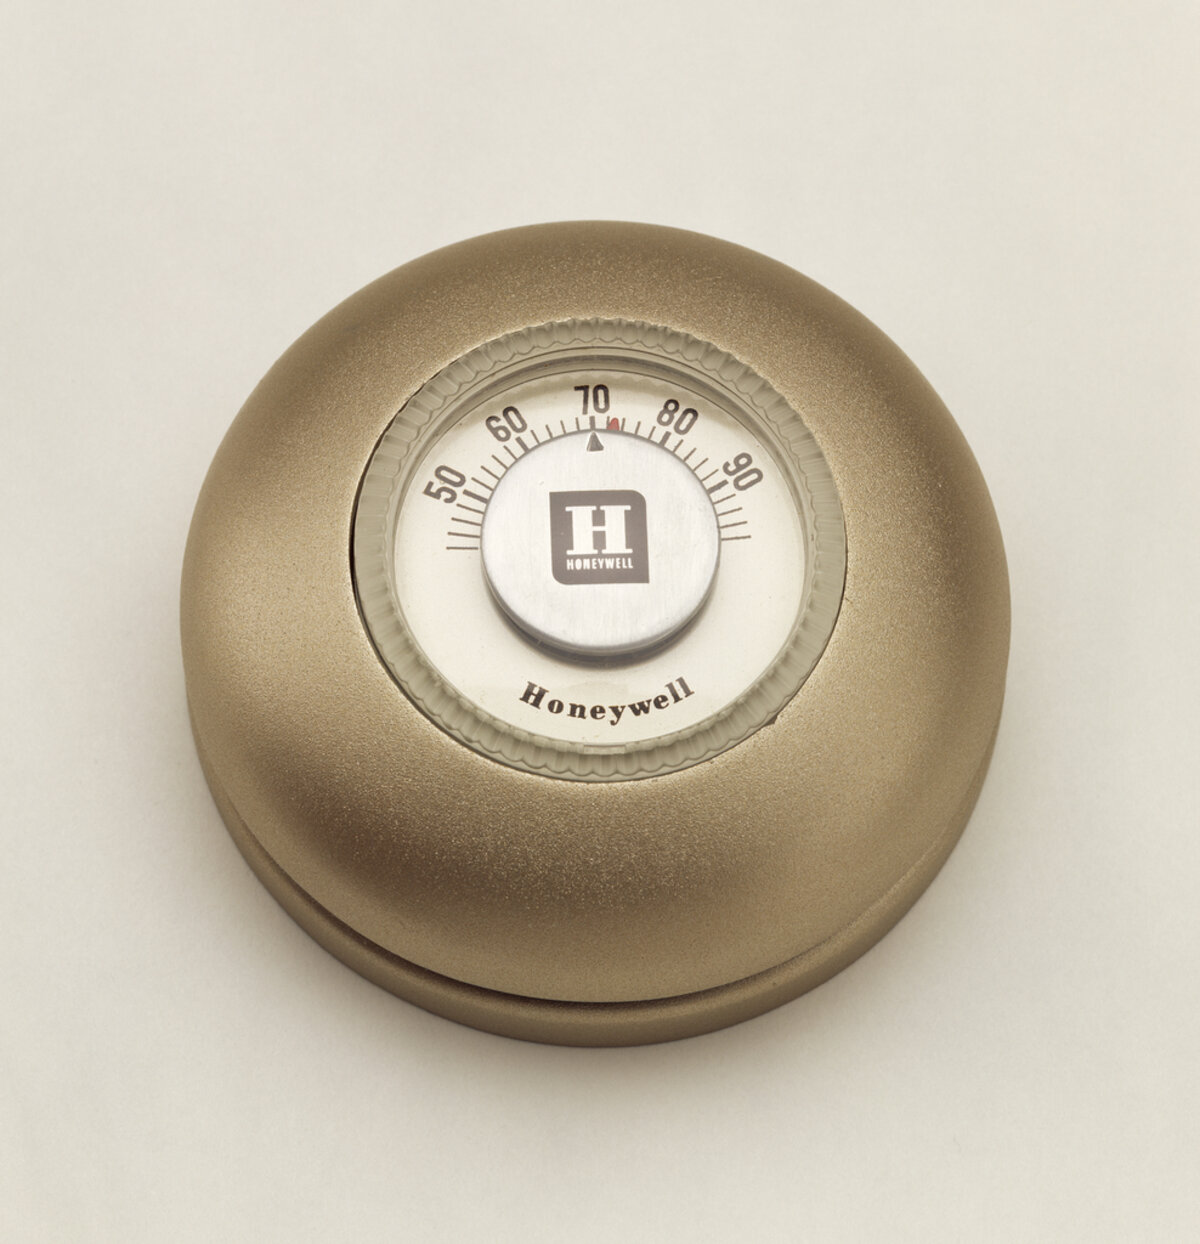
\includegraphics[width=\linewidth,height=0.70\textheight,keepaspectratio]{images-companion/ch04_pid.jpg}

\caption{Figure C4.6: Honeywell Round Thermostat (1953) — Classic Bang-Bang/PID Feedback Control}

\end{figure}

\begin{figure}[H]

\hypertarget{fig-c4-7}{}\label{fig-c4-7}

\centering

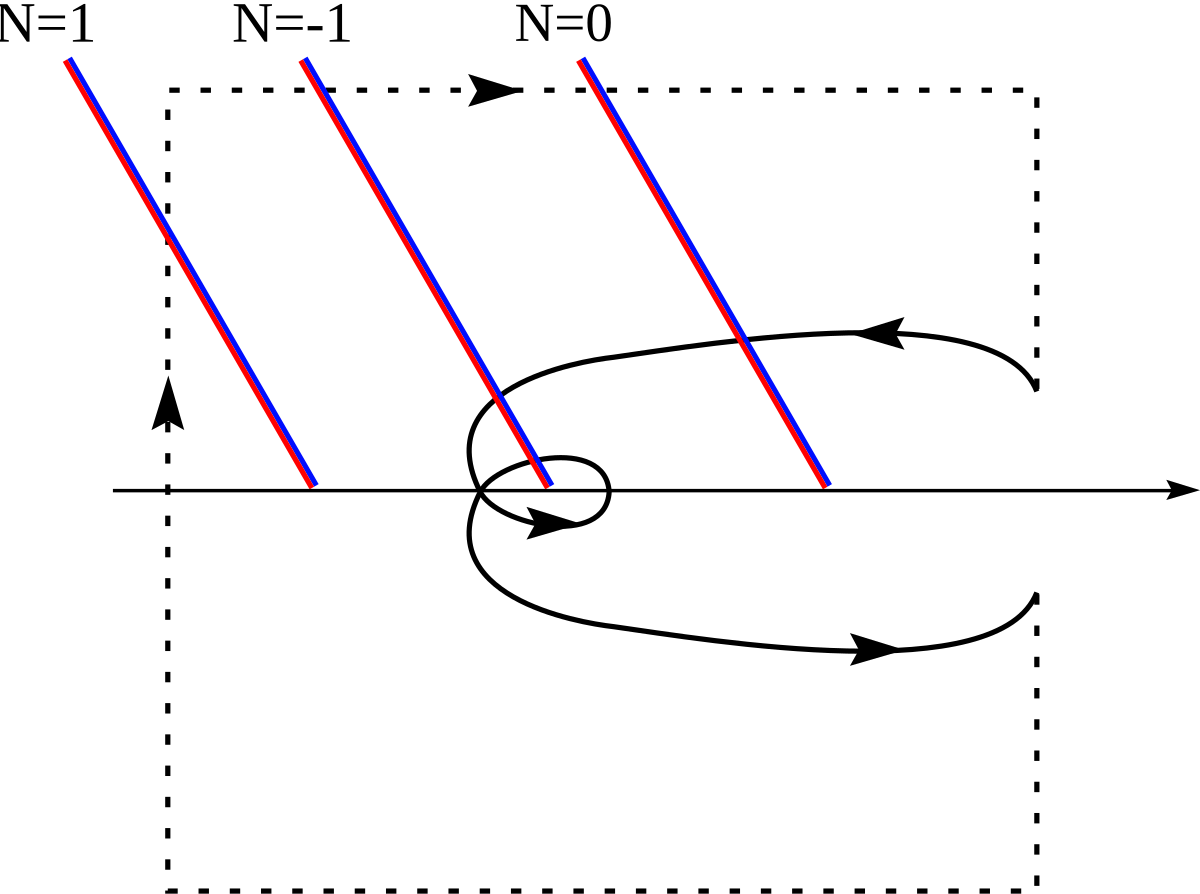
\includegraphics[width=\linewidth,height=0.70\textheight,keepaspectratio]{images-companion/ch04_stability.png}

\caption{Figure C4.7: Nyquist Stability Criterion Diagram}

\end{figure}

\begin{figure}[H]

\hypertarget{fig-c4-8}{}\label{fig-c4-8}

\centering

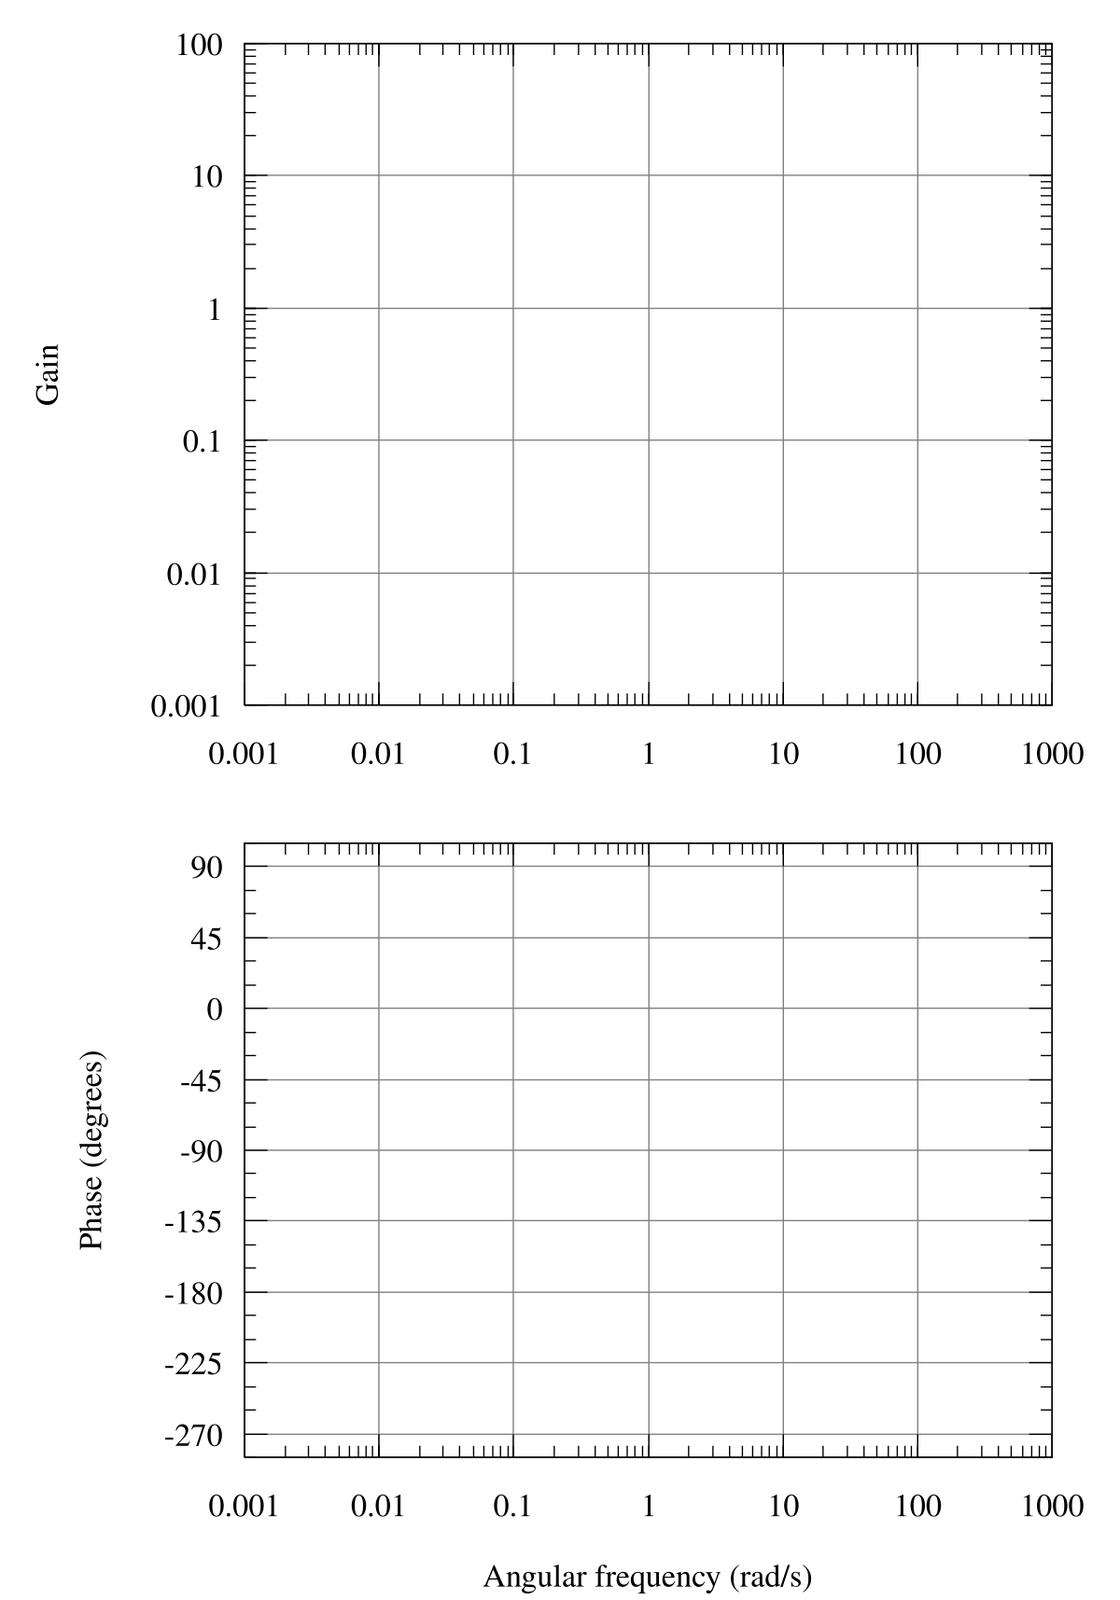
\includegraphics[width=\linewidth,height=0.70\textheight,keepaspectratio]{images-companion/ch04_freqresponse.png}

\caption{Figure C4.8: Bode Plot Template — Magnitude and Phase vs. Frequency}

\end{figure}

\begin{figure}[H]

\hypertarget{fig-c4-9}{}\label{fig-c4-9}

\centering

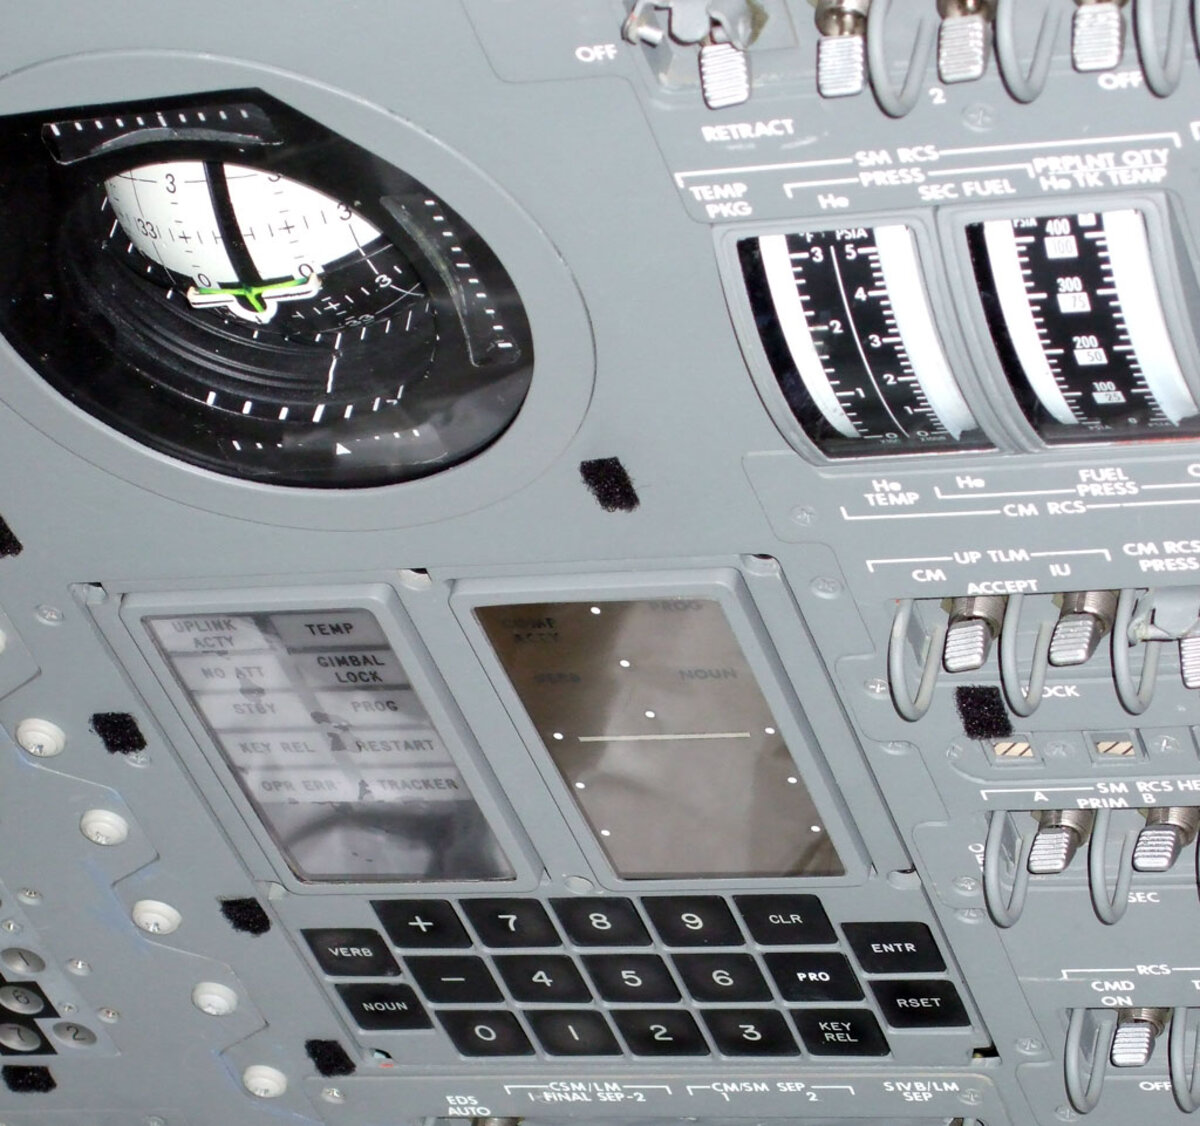
\includegraphics[width=\linewidth,height=0.70\textheight,keepaspectratio]{images-companion/ch04_statespace.jpg}

\caption{Figure C4.9: Apollo Guidance Computer DSKY (Display and Keyboard) — Onboard State Estimation and Control Interface}

\end{figure}

\begin{figure}[H]

\hypertarget{fig-c4-10}{}\label{fig-c4-10}

\centering

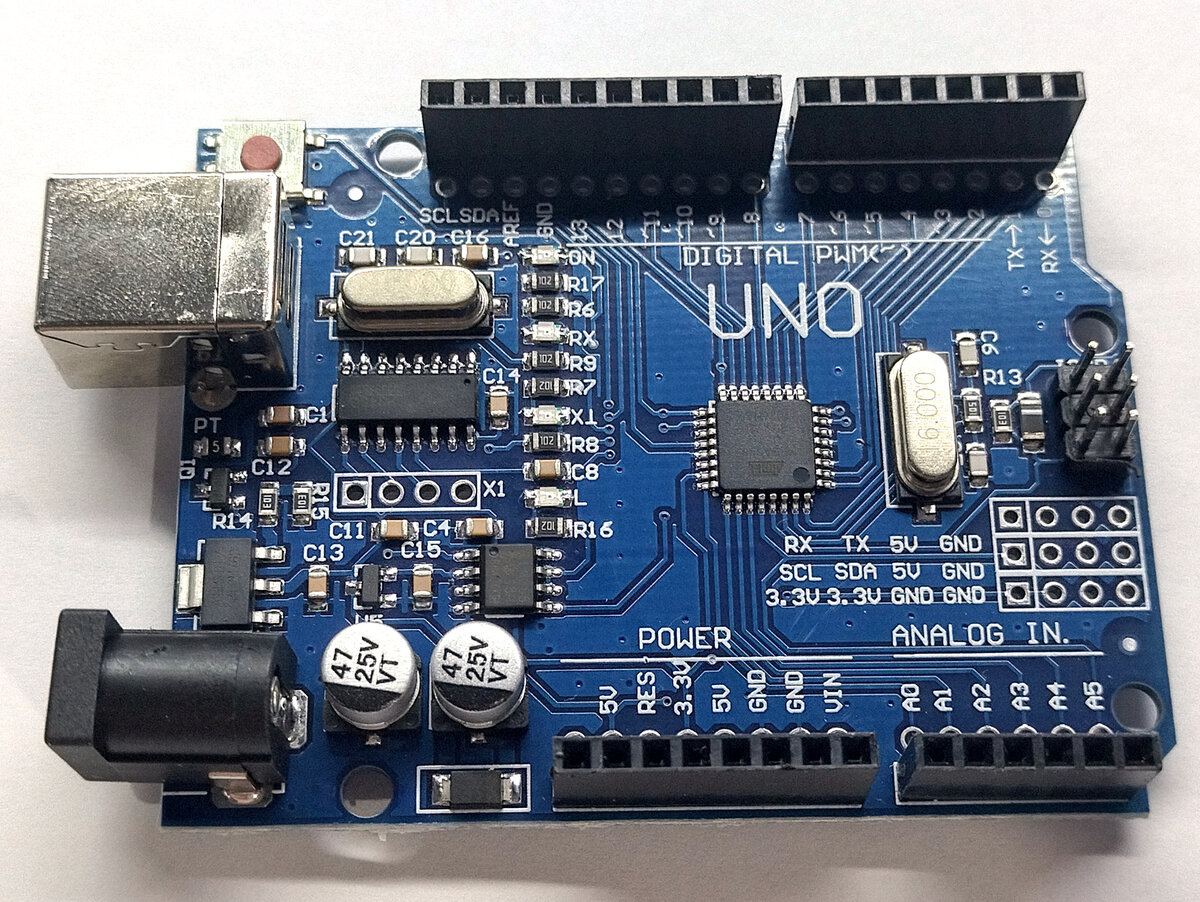
\includegraphics[width=\linewidth,height=0.70\textheight,keepaspectratio]{images-companion/ch04_digitalcontrol.jpg}

\caption{Figure C4.10: Arduino Uno Microcontroller Board — a Common Digital Control System Platform}

\end{figure}

\section{Chapter 5: Embedded Systems}\label{chapter-5-embedded-systems}

\begin{figure}[H]

\hypertarget{fig-c5-1}{}\label{fig-c5-1}

\centering

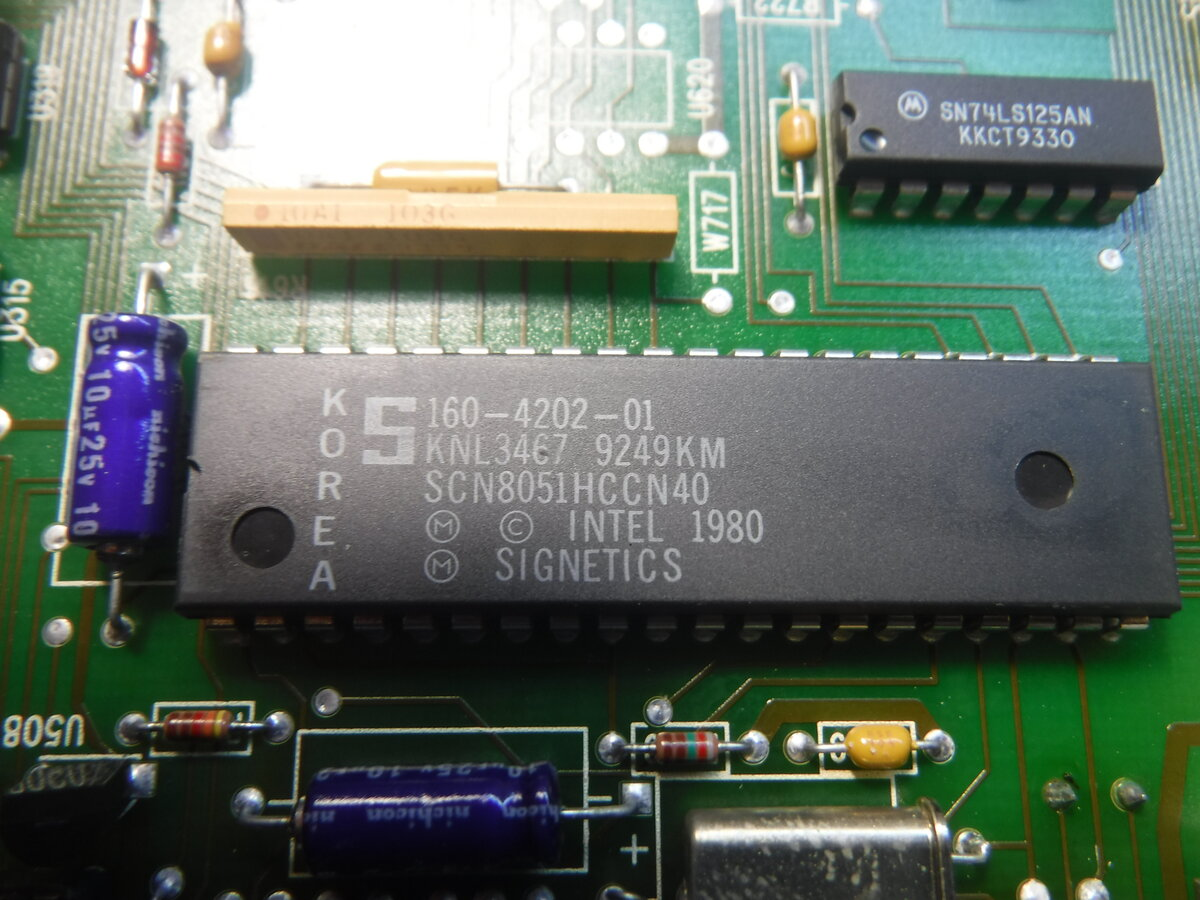
\includegraphics[width=\linewidth,height=0.70\textheight,keepaspectratio]{images-companion/ch05_microcontroller.jpg}

\caption{Figure C5.1: Signetics SCN8051 (Intel 8051-Compatible) Microcontroller on a Circuit Board}

\end{figure}

\begin{figure}[H]

\hypertarget{fig-c5-2}{}\label{fig-c5-2}

\centering

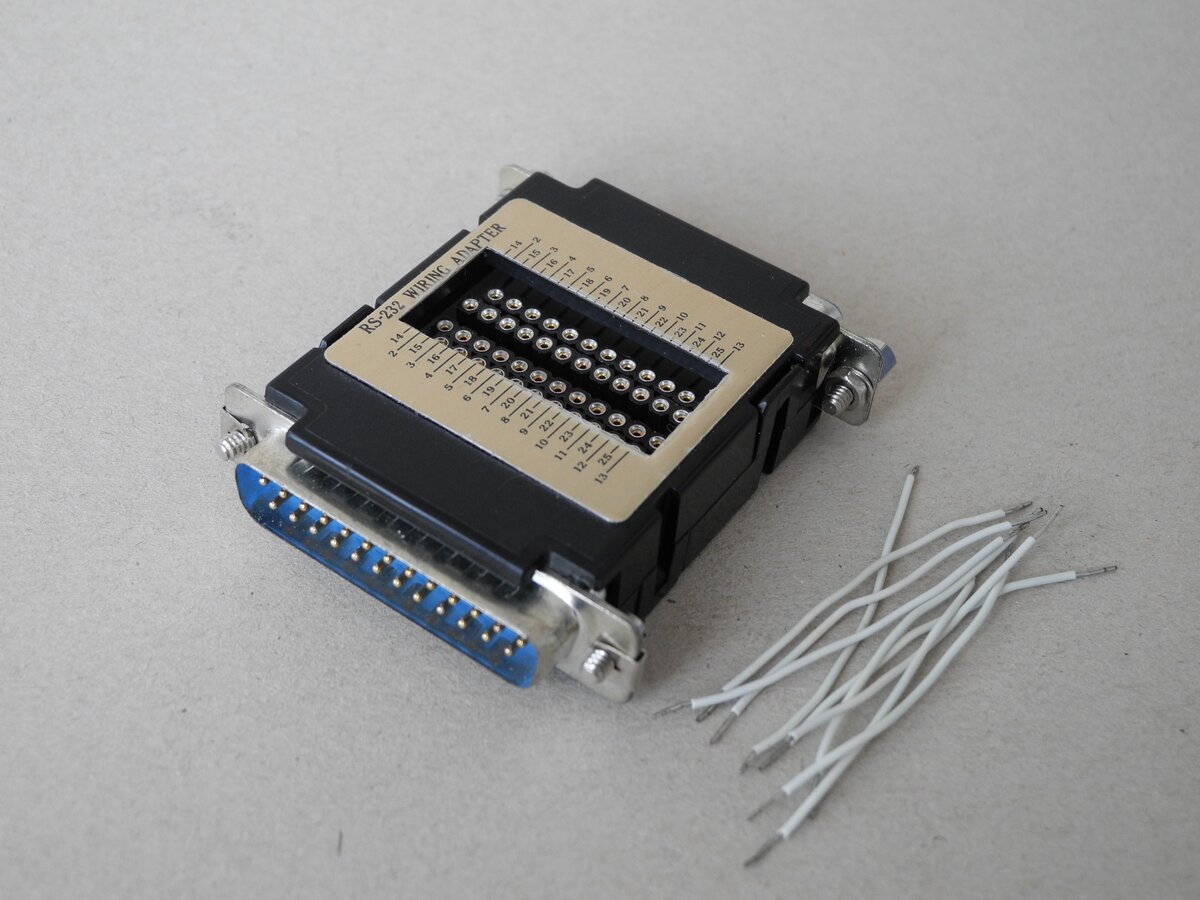
\includegraphics[width=\linewidth,height=0.70\textheight,keepaspectratio]{images-companion/ch05_comm.jpg}

\caption{Figure C5.2: RS-232 Wiring Adapter (DB-25) for Serial Communication Interfaces}

\end{figure}

\section{Chapter 6: Digital Logic}\label{chapter-6-digital-logic}

\begin{figure}[H]

\hypertarget{fig-c6-1}{}\label{fig-c6-1}

\centering

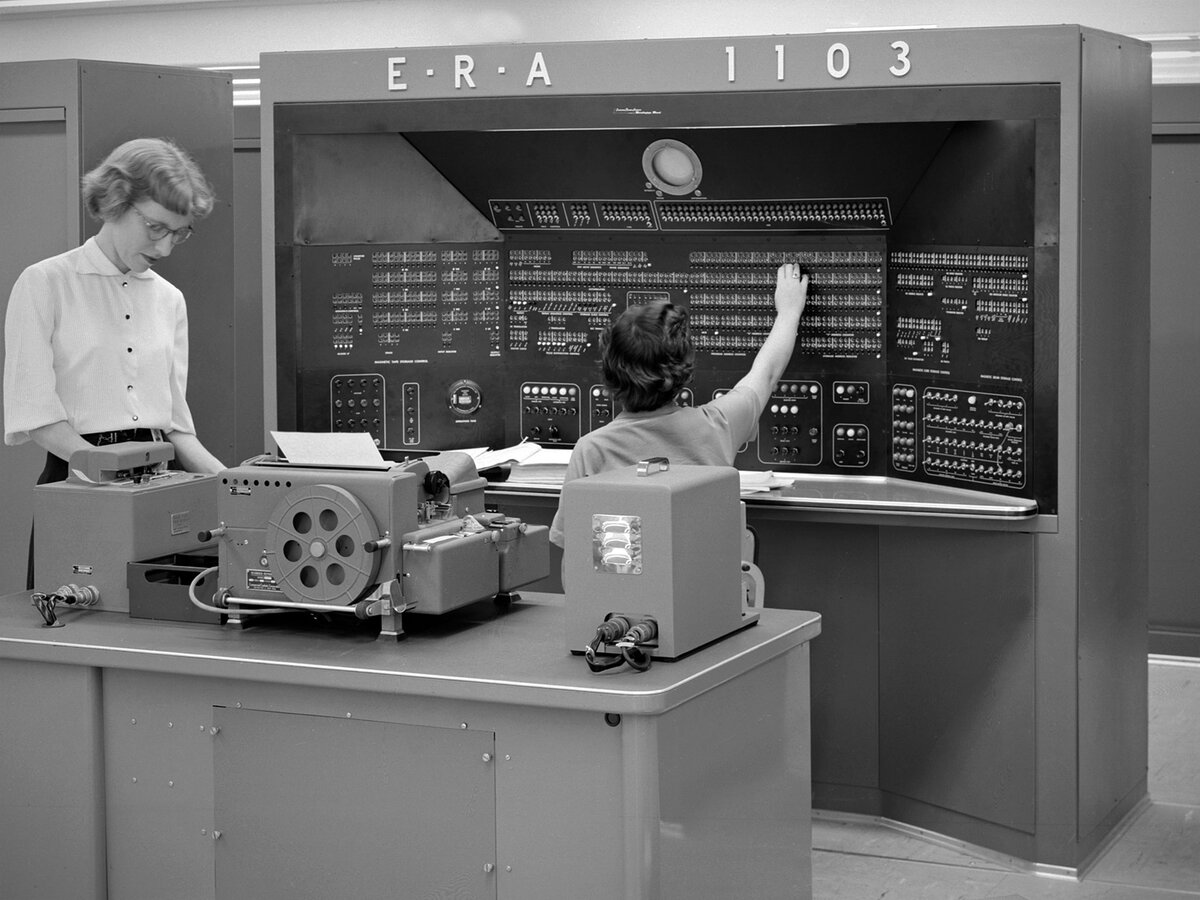
\includegraphics[width=\linewidth,height=0.70\textheight,keepaspectratio]{images-companion/ch06_numbers.jpg}

\caption{Figure C6.1: ERA 1103 Computer — Early Binary/Digital Calculating Machine (1955)}

\end{figure}

\begin{figure}[H]

\hypertarget{fig-c6-2}{}\label{fig-c6-2}

\centering

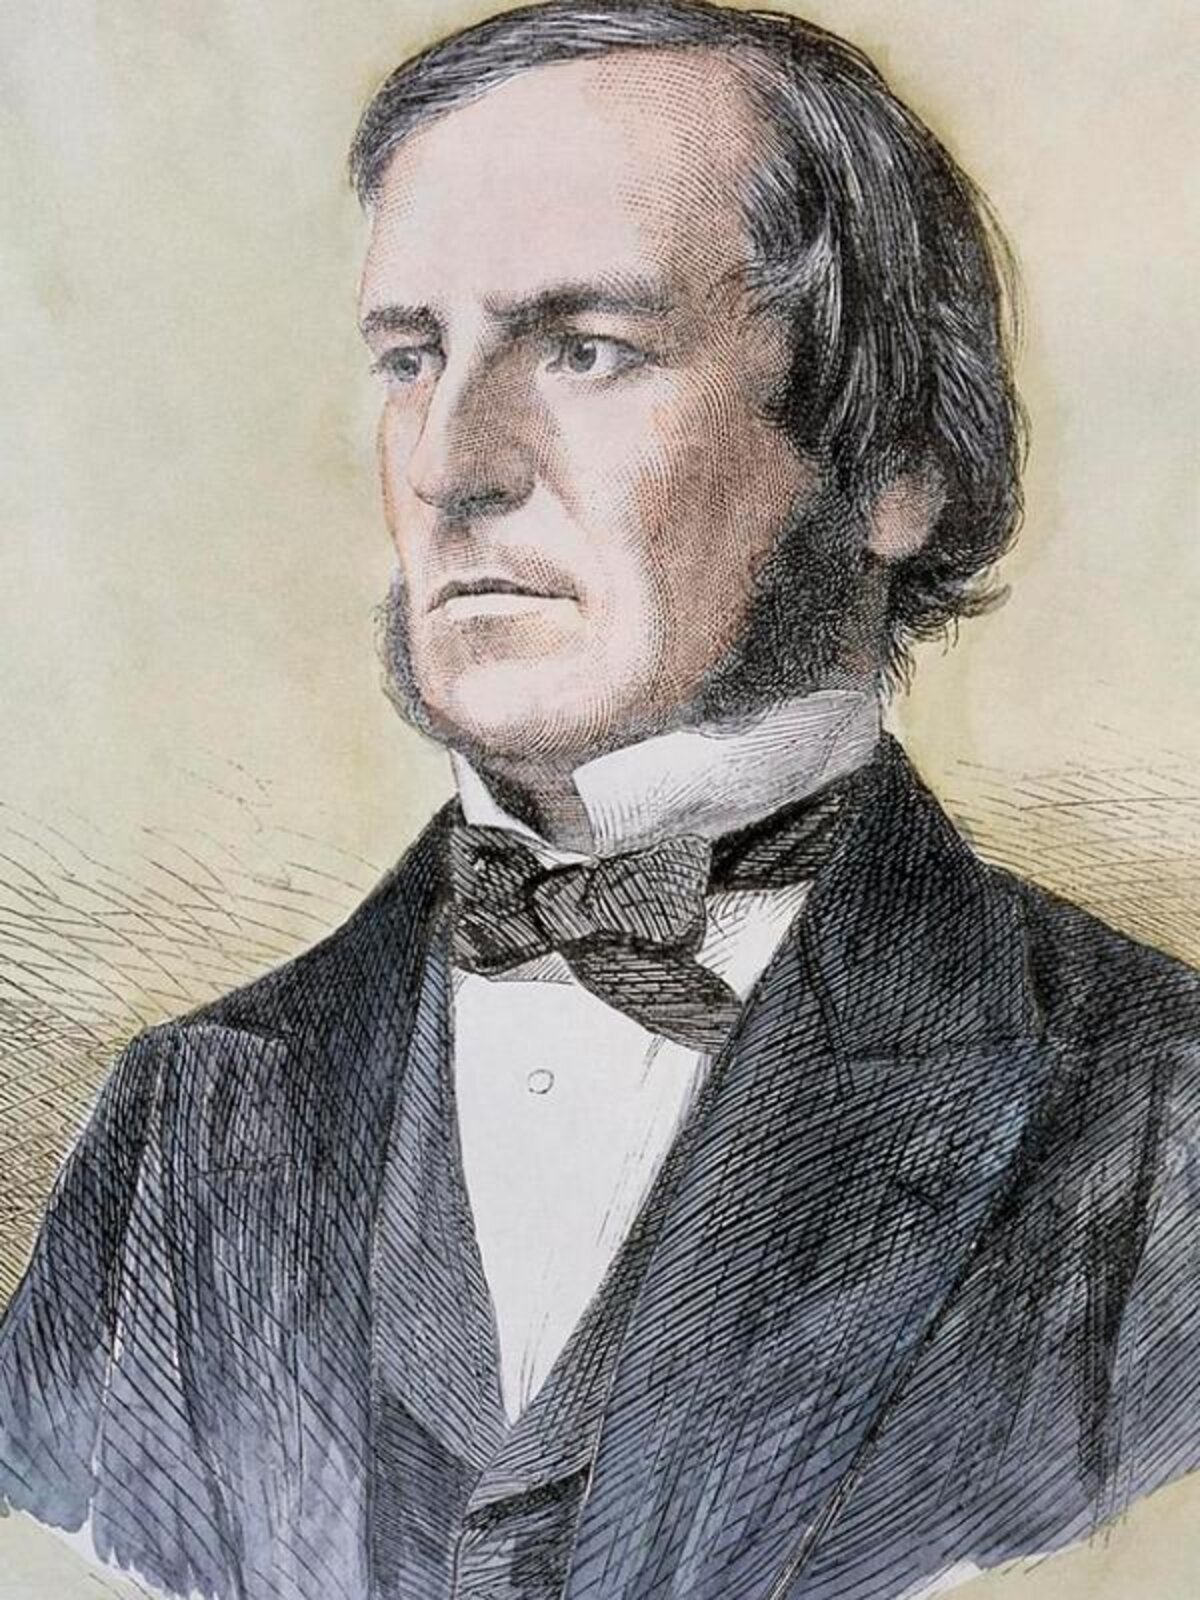
\includegraphics[width=\linewidth,height=0.70\textheight,keepaspectratio]{images-companion/ch06_boolean.jpg}

\caption{Figure C6.2: George Boole, Originator of Boolean Algebra}

\end{figure}

\begin{figure}[H]

\hypertarget{fig-c6-3}{}\label{fig-c6-3}

\centering

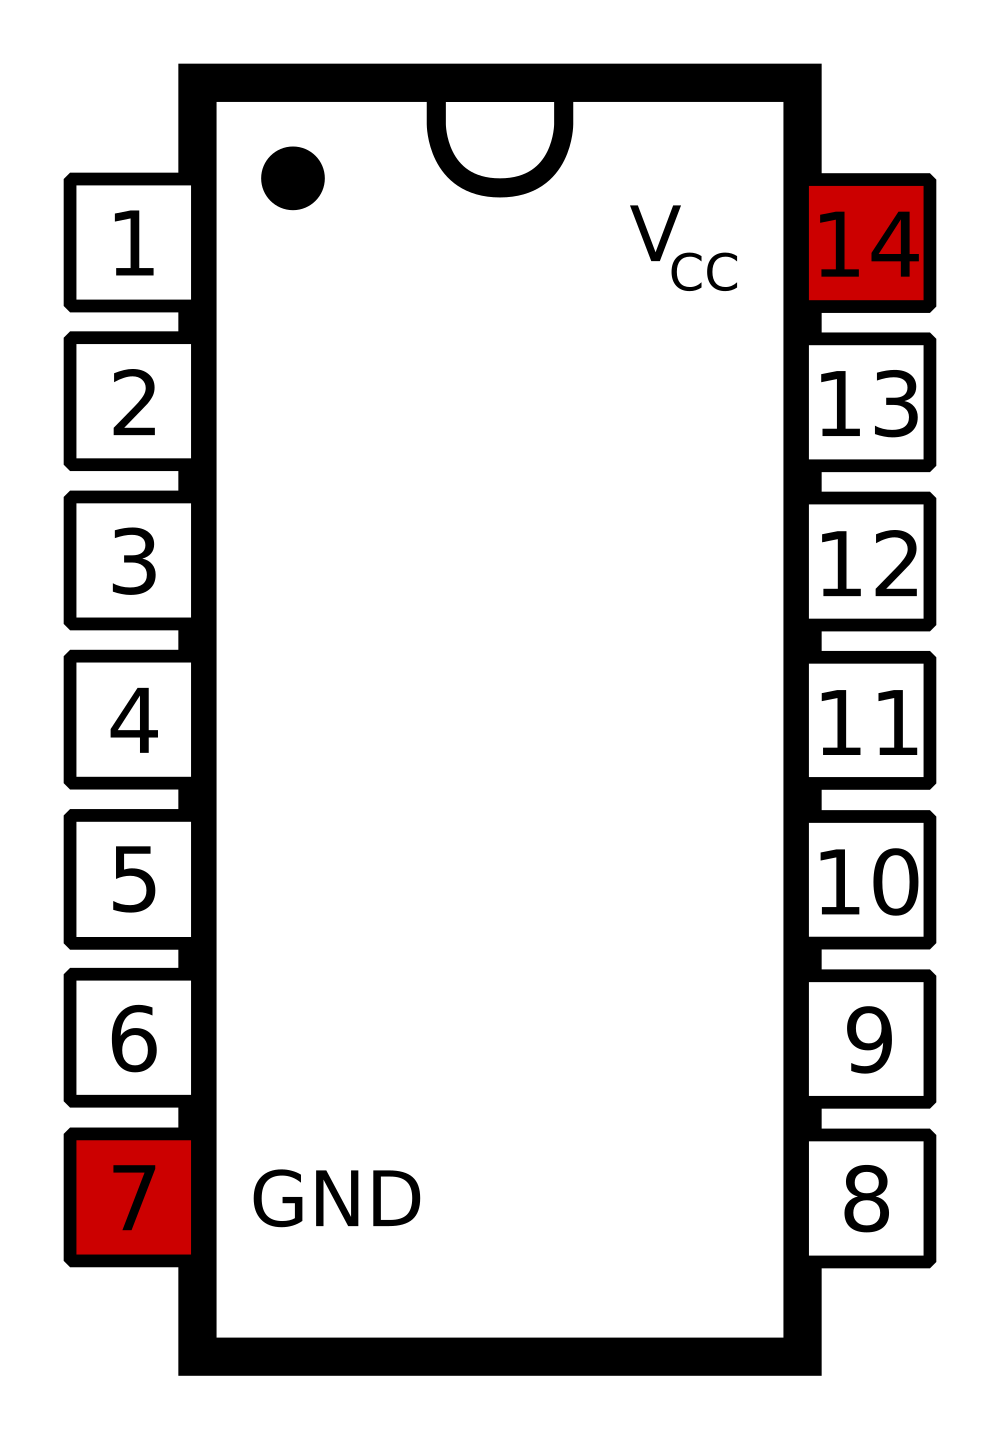
\includegraphics[width=\linewidth,height=0.70\textheight,keepaspectratio]{images-companion/ch06_gates.png}

\caption{Figure C6.3: Generic 14-Pin TTL Logic Gate IC Pinout}

\end{figure}

\begin{figure}[H]

\hypertarget{fig-c6-4}{}\label{fig-c6-4}

\centering

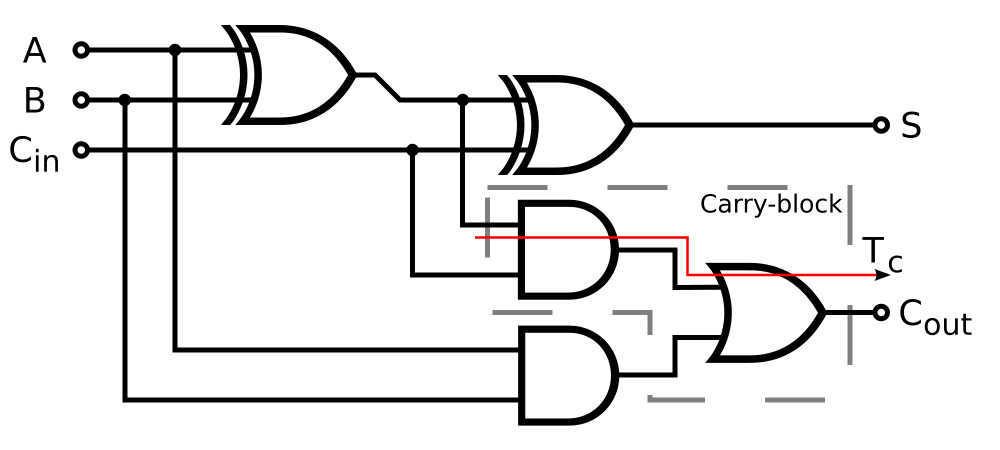
\includegraphics[width=\linewidth,height=0.70\textheight,keepaspectratio]{images-companion/ch06_combinational.png}

\caption{Figure C6.4: Full-Adder Combinational Logic Diagram}

\end{figure}

\begin{figure}[H]

\hypertarget{fig-c6-5}{}\label{fig-c6-5}

\centering

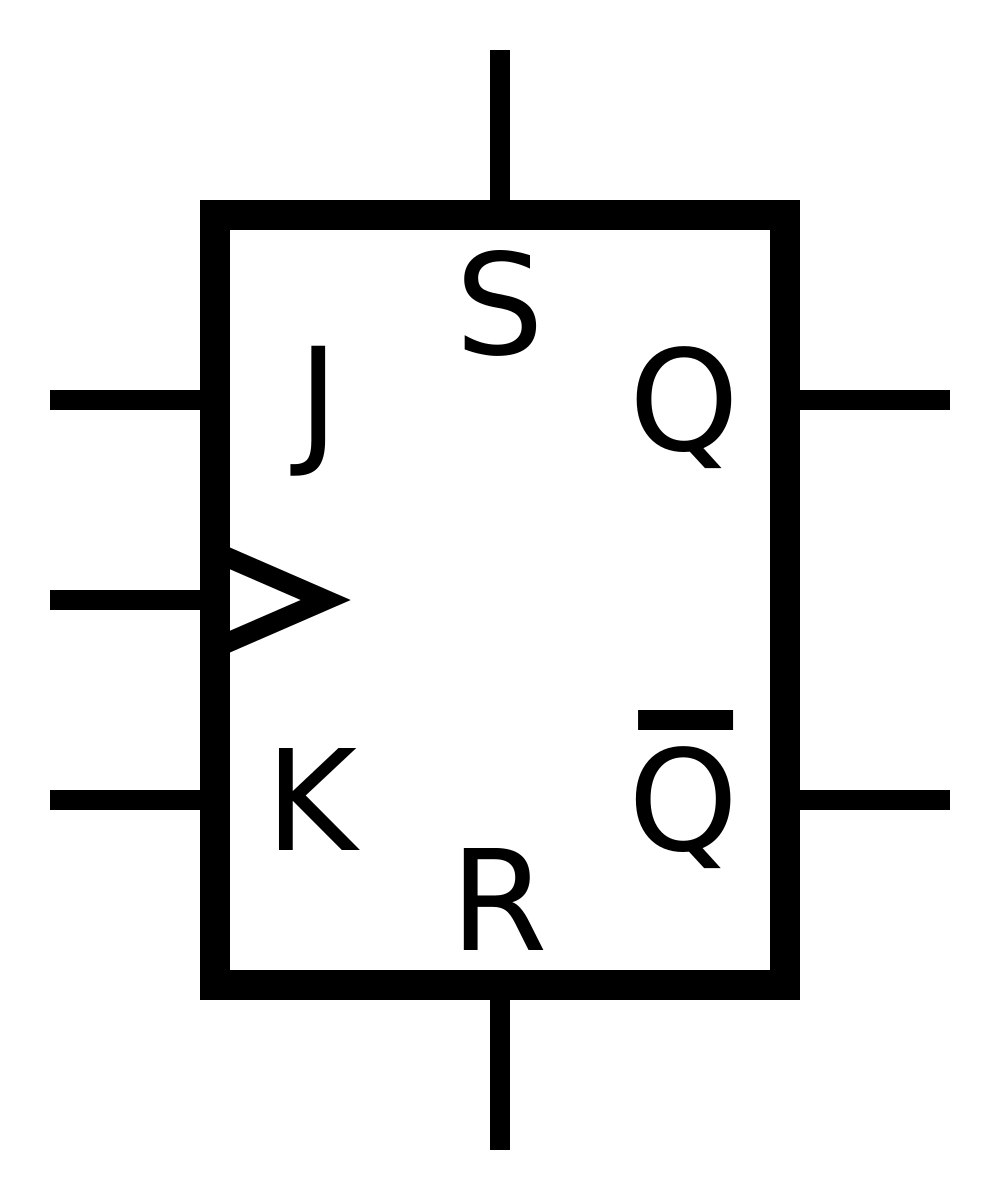
\includegraphics[width=\linewidth,height=0.70\textheight,keepaspectratio]{images-companion/ch06_sequential.png}

\caption{Figure C6.5: JK Flip-Flop Sequential Logic Diagram}

\end{figure}

\section{Chapter 7: Circuit Analysis}\label{chapter-7-circuit-analysis}

\begin{figure}[H]

\hypertarget{fig-c7-1}{}\label{fig-c7-1}

\centering

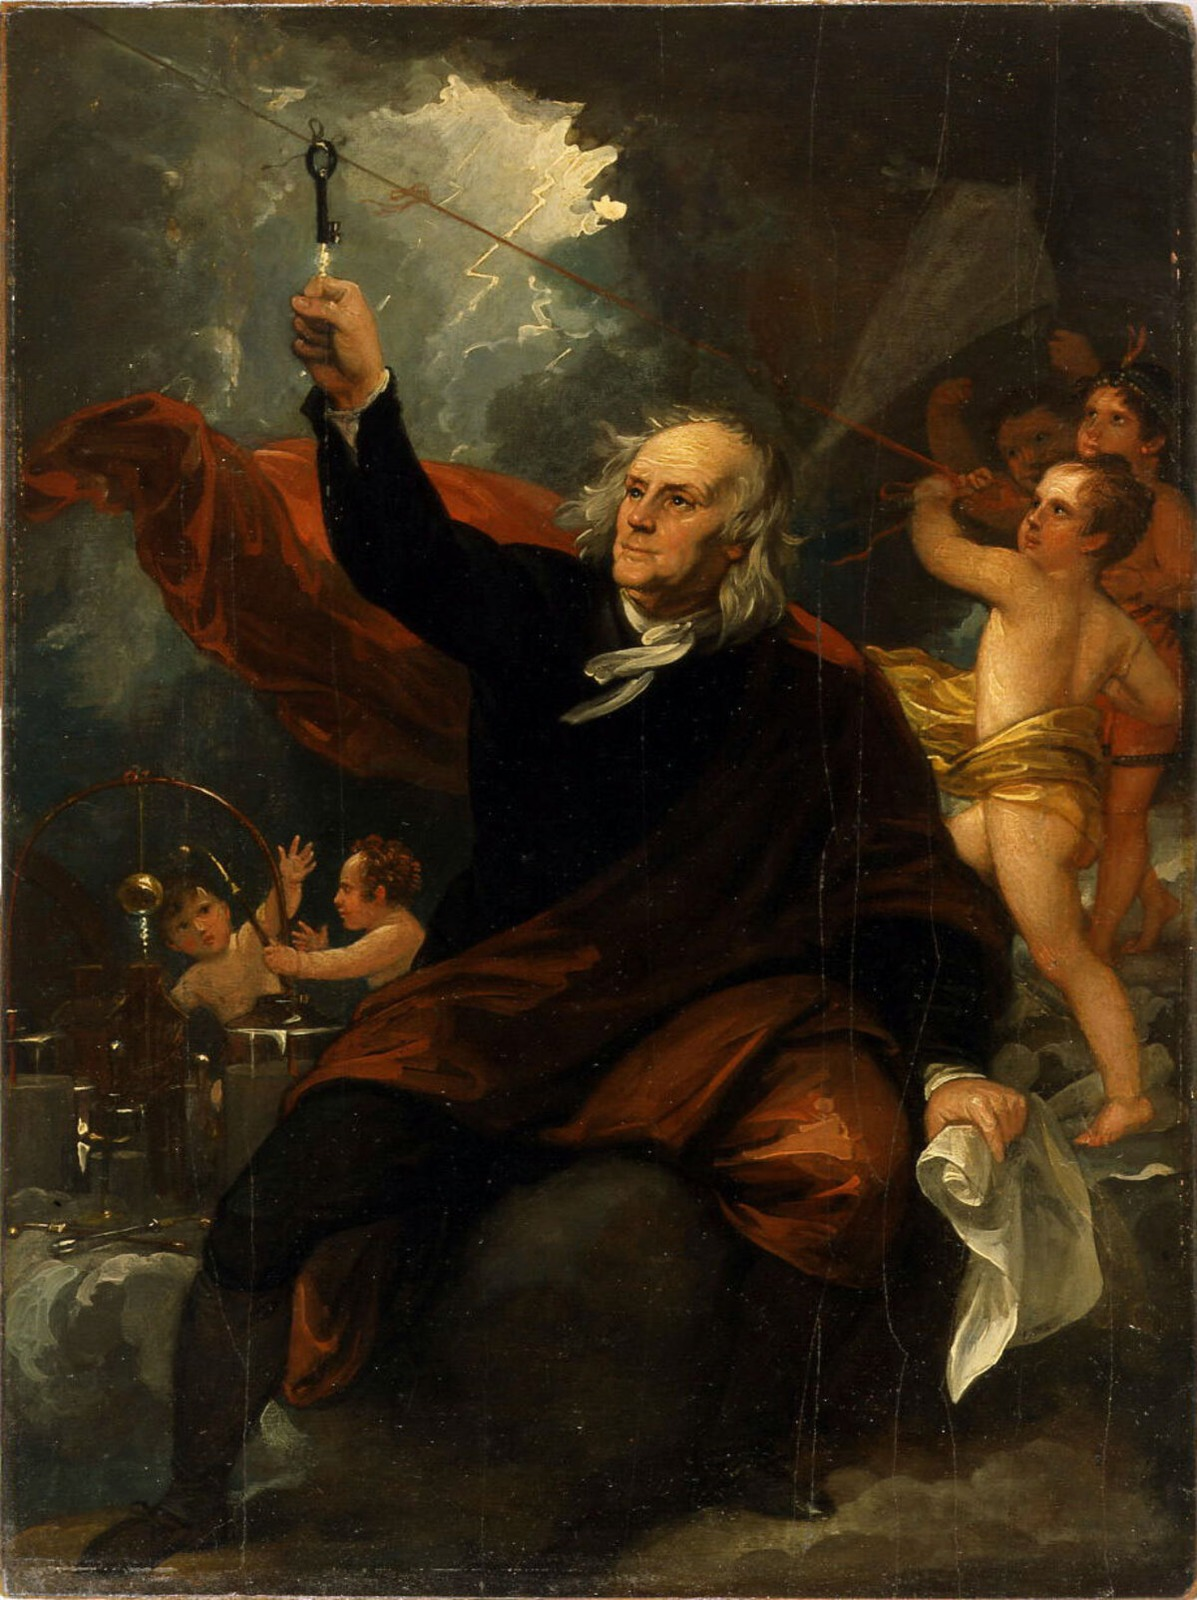
\includegraphics[width=\linewidth,height=0.70\textheight,keepaspectratio]{images-companion/ch07_charge.jpg}

\caption{Figure C7.1: Benjamin Franklin Drawing Electricity from the Sky (Benjamin West, c. 1816)}

\end{figure}

\begin{figure}[H]

\hypertarget{fig-c7-3}{}\label{fig-c7-3}

\centering

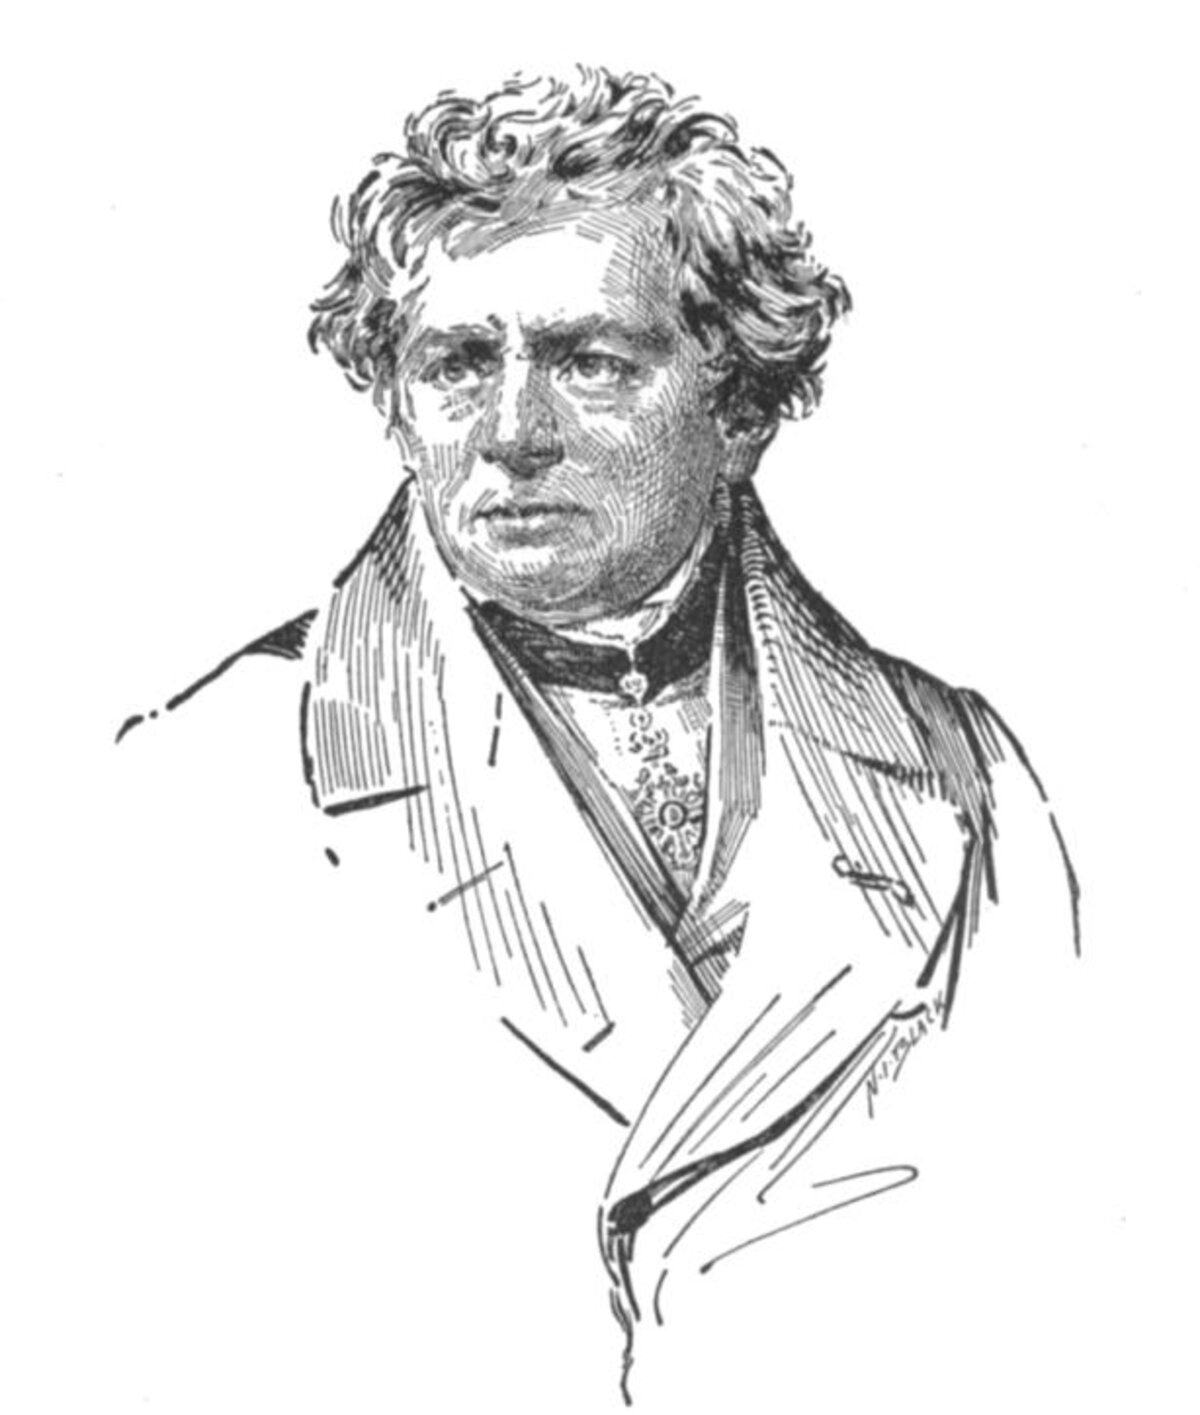
\includegraphics[width=\linewidth,height=0.70\textheight,keepaspectratio]{images-companion/ch07_ohm.jpg}

\caption{Figure C7.3: Georg Simon Ohm, Namesake of Ohm’s Law}

\end{figure}

\begin{figure}[H]

\hypertarget{fig-c7-4}{}\label{fig-c7-4}

\centering

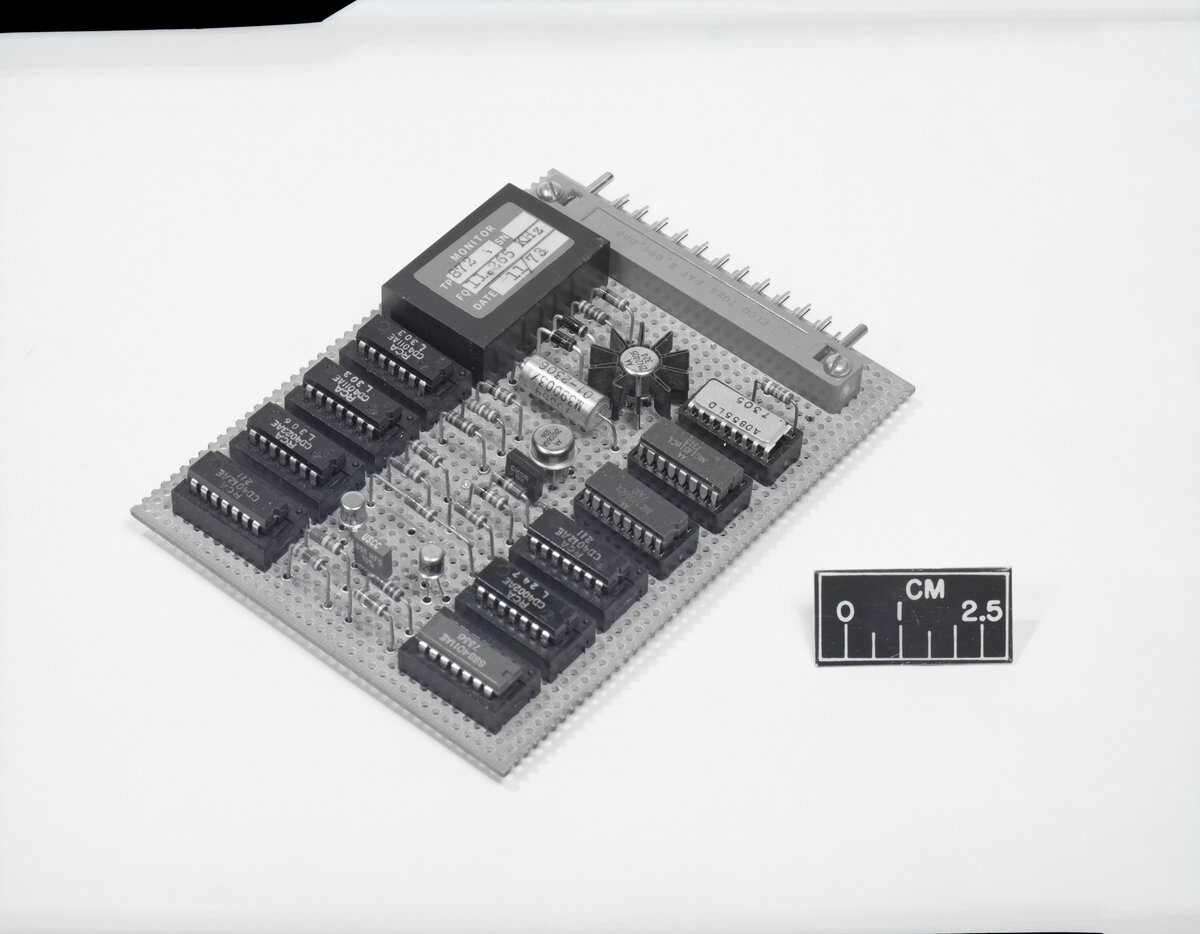
\includegraphics[width=\linewidth,height=0.70\textheight,keepaspectratio]{images-companion/ch07_dcanalysis.jpg}

\caption{Figure C7.4: Populated DC Circuit Board on Breadboard-Style Perfboard}

\end{figure}

\begin{figure}[H]

\hypertarget{fig-c7-5}{}\label{fig-c7-5}

\centering

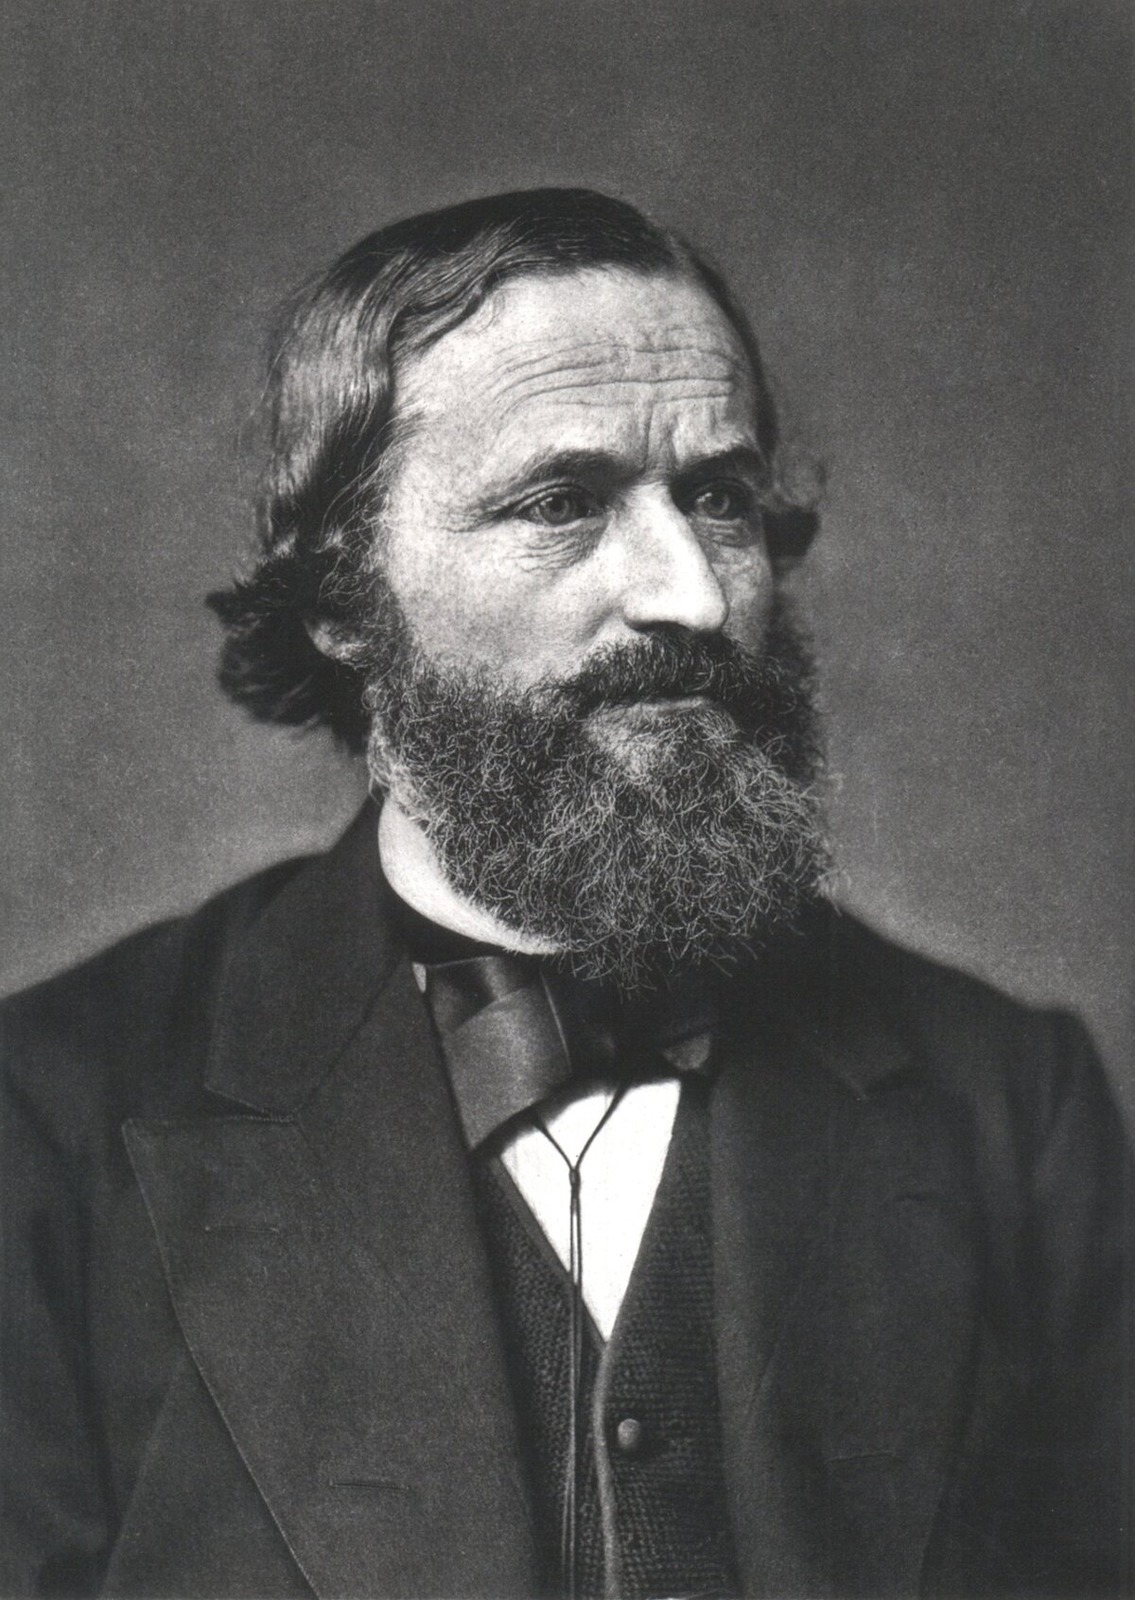
\includegraphics[width=\linewidth,height=0.70\textheight,keepaspectratio]{images-companion/ch07_kirchhoff.jpg}

\caption{Figure C7.5: Gustav Robert Kirchhoff, Originator of Kirchhoff’s Circuit Laws}

\end{figure}

\begin{figure}[H]

\hypertarget{fig-c7-6}{}\label{fig-c7-6}

\centering

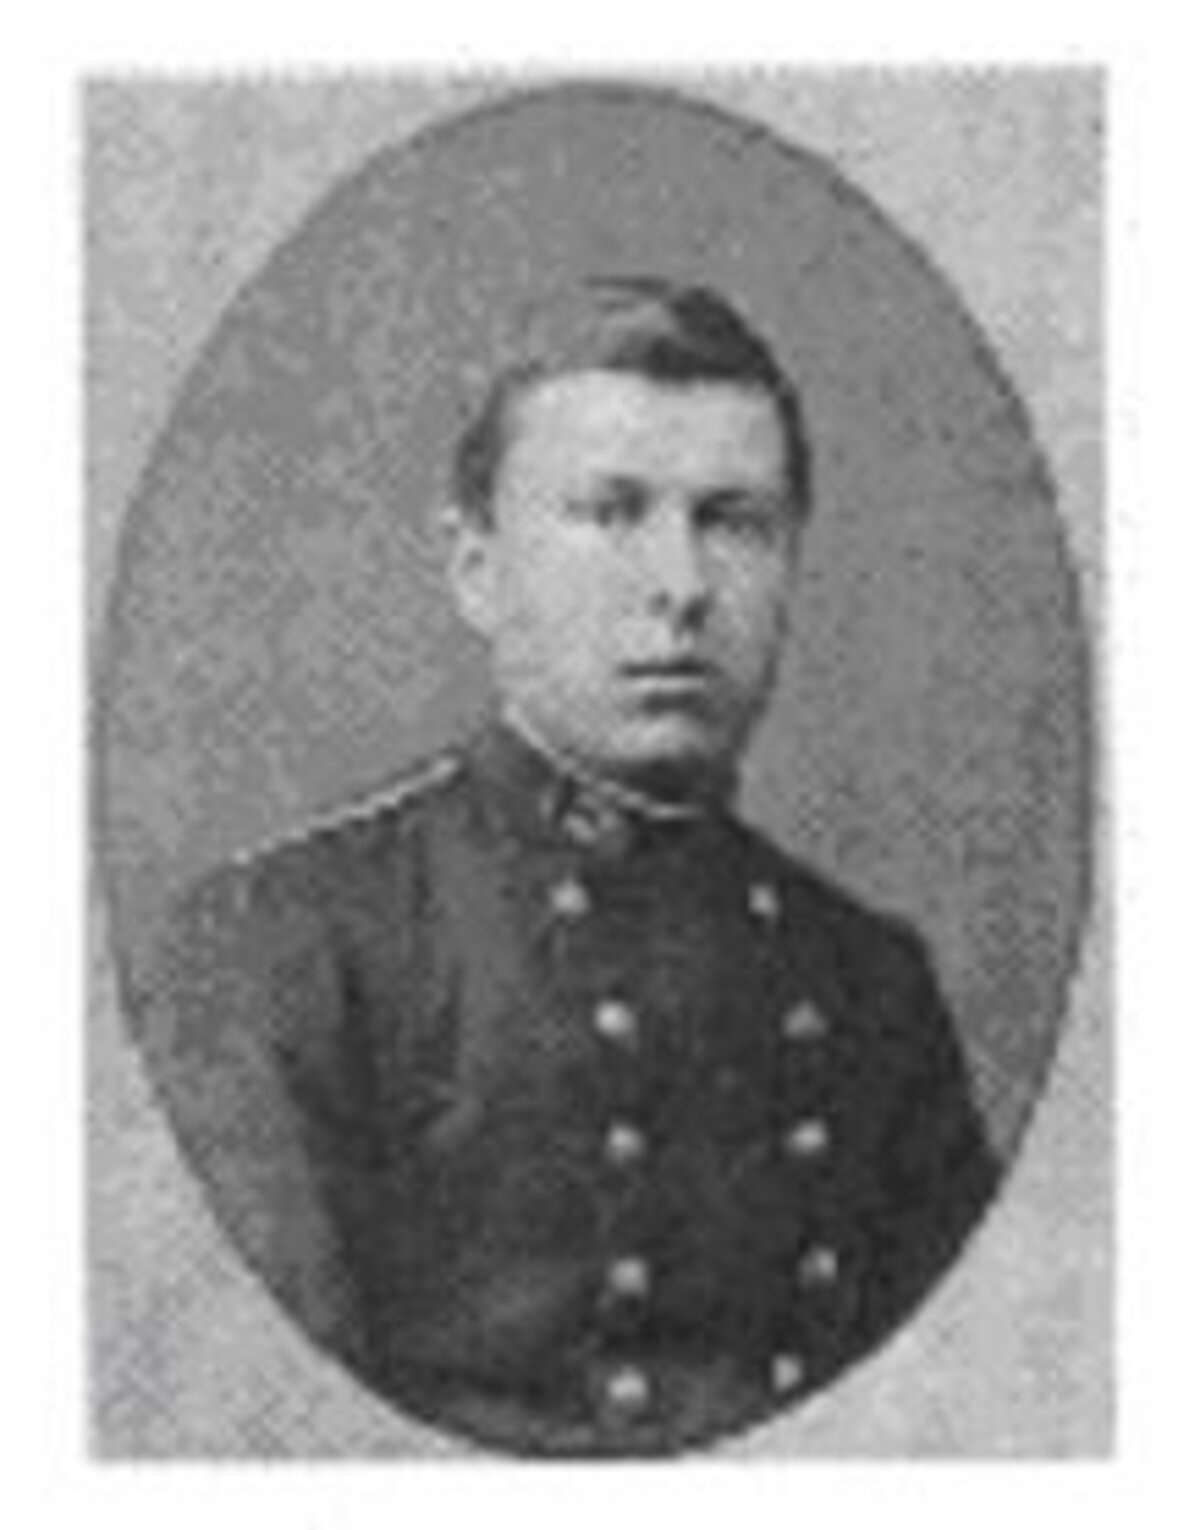
\includegraphics[width=\linewidth,height=0.70\textheight,keepaspectratio]{images-companion/ch07_thevenin.jpg}

\caption{Figure C7.6: Léon Charles Thévenin, Namesake of Thévenin’s Theorem}

\end{figure}

\begin{figure}[H]

\hypertarget{fig-c7-7}{}\label{fig-c7-7}

\centering

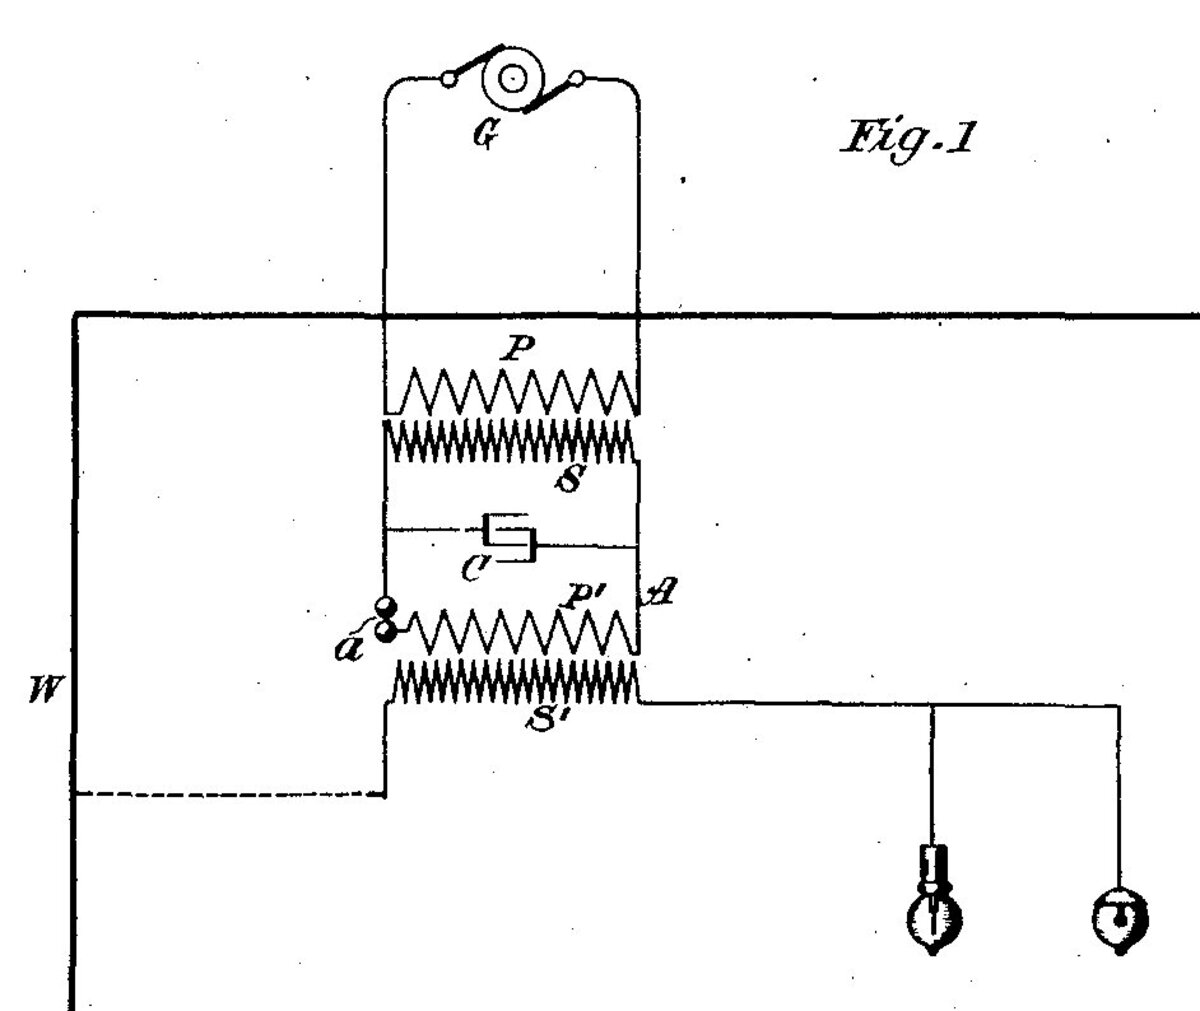
\includegraphics[width=\linewidth,height=0.70\textheight,keepaspectratio]{images-companion/ch07_actheory.jpg}

\caption{Figure C7.7: Nikola Tesla’s 1891 Patent Drawing for a System of Electric (AC) Lighting}

\end{figure}

\begin{figure}[H]

\hypertarget{fig-c7-9}{}\label{fig-c7-9}

\centering

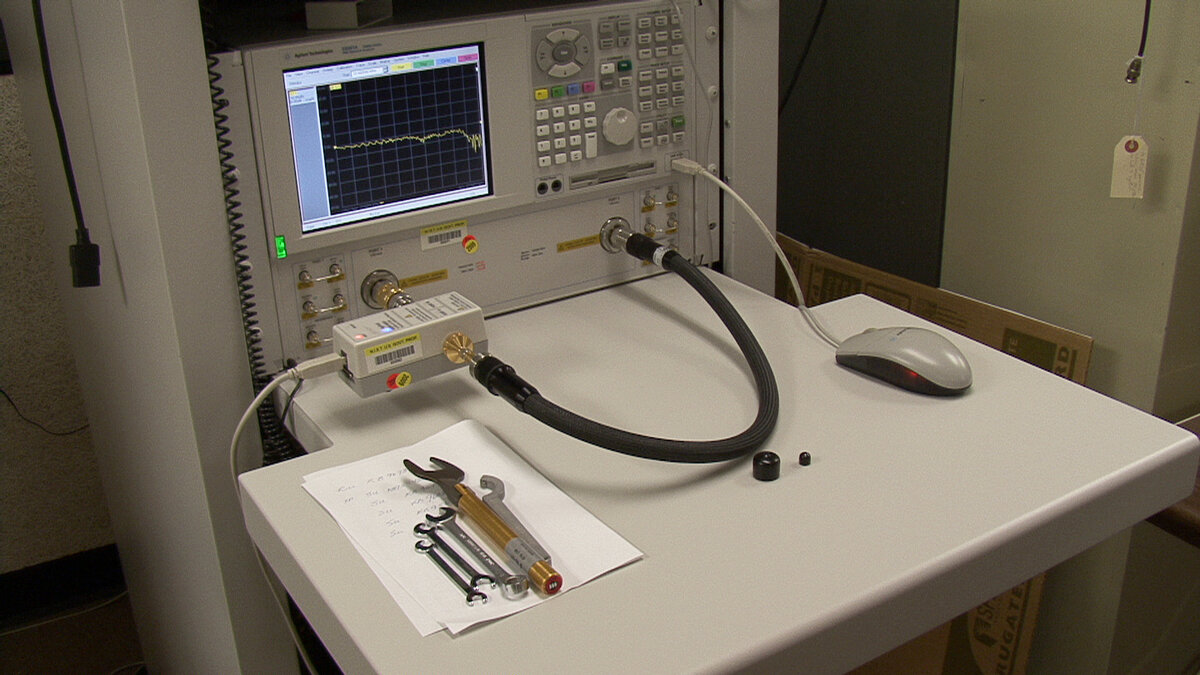
\includegraphics[width=\linewidth,height=0.70\textheight,keepaspectratio]{images-companion/ch07_twoport.jpg}

\caption{Figure C7.9: Vector Network Analyzer Used for Two-Port Network Calibration}

\end{figure}

\section{Chapter 8: Signal
Processing}\label{chapter-8-signal-processing}

\begin{figure}[H]

\hypertarget{fig-c8-1}{}\label{fig-c8-1}

\centering

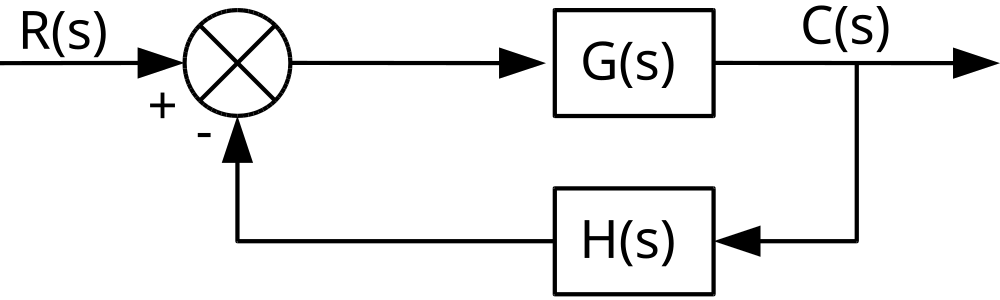
\includegraphics[width=\linewidth,height=0.70\textheight,keepaspectratio]{images-companion/ch08_signals.png}

\caption{Figure C8.1: General Closed-Loop Feedback System Block Diagram}

\end{figure}

\begin{figure}[H]

\hypertarget{fig-c8-2}{}\label{fig-c8-2}

\centering

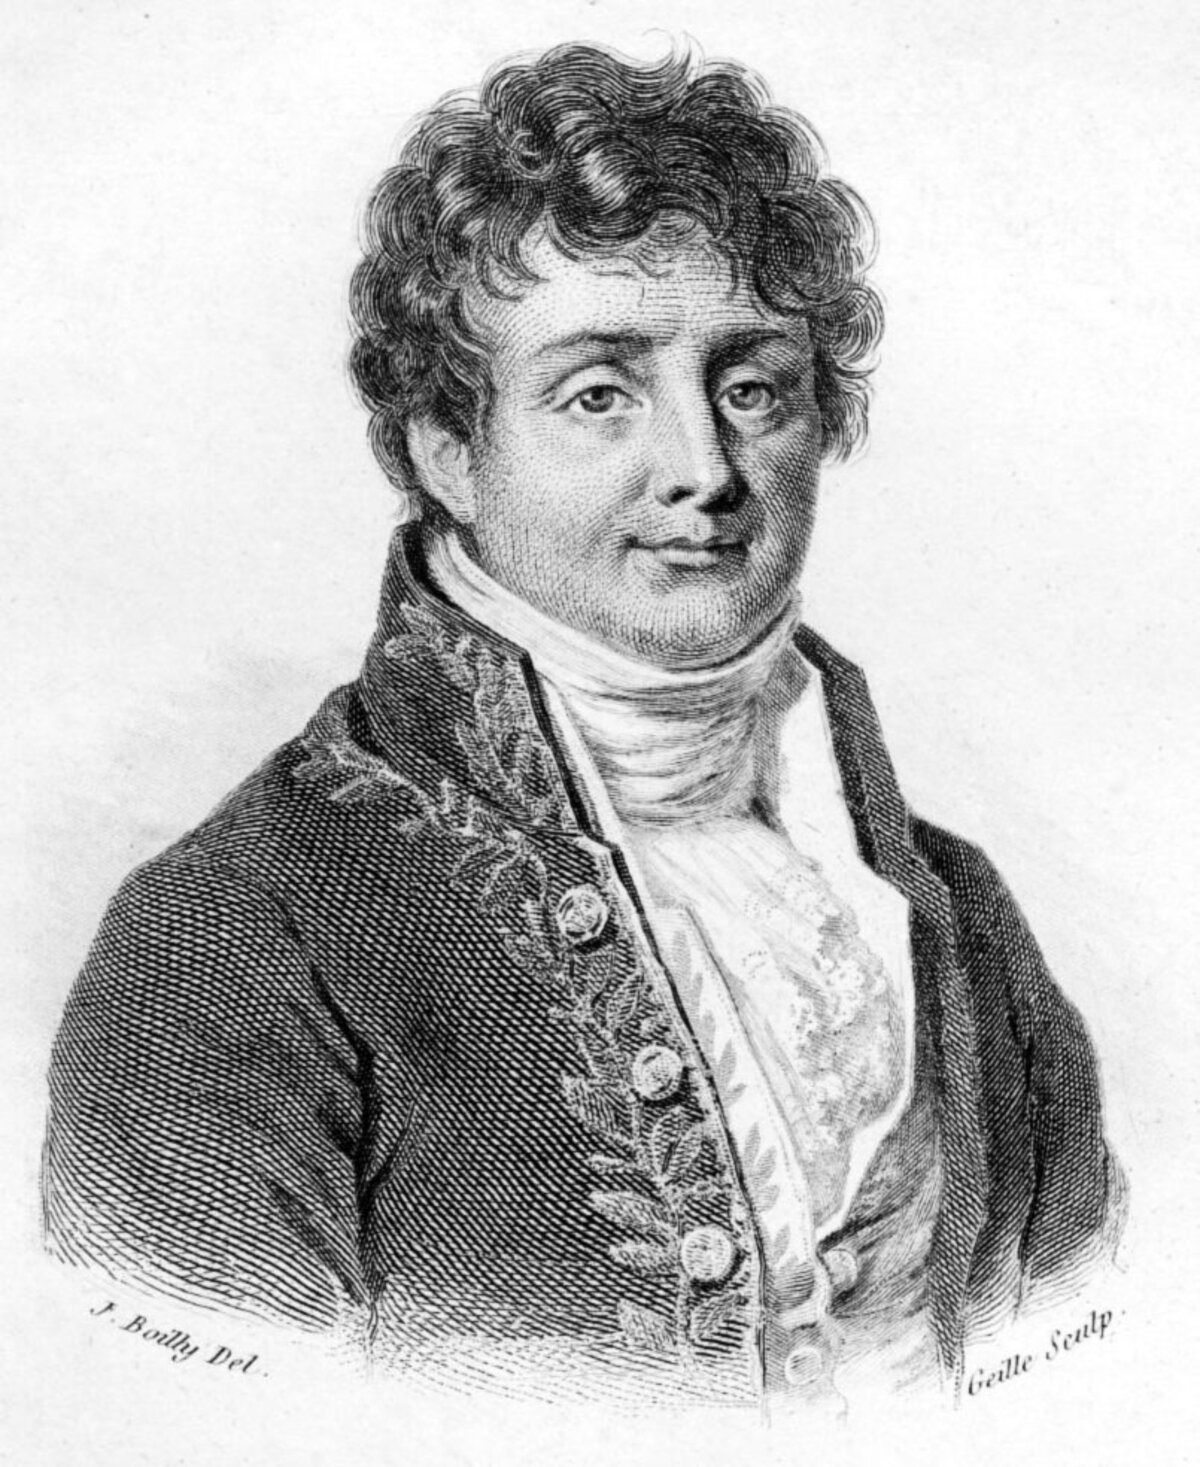
\includegraphics[width=\linewidth,height=0.70\textheight,keepaspectratio]{images-companion/ch08_fourier.jpg}

\caption{Figure C8.2: Joseph Fourier, Originator of Fourier Analysis}

\end{figure}

\begin{figure}[H]

\hypertarget{fig-c8-3}{}\label{fig-c8-3}

\centering

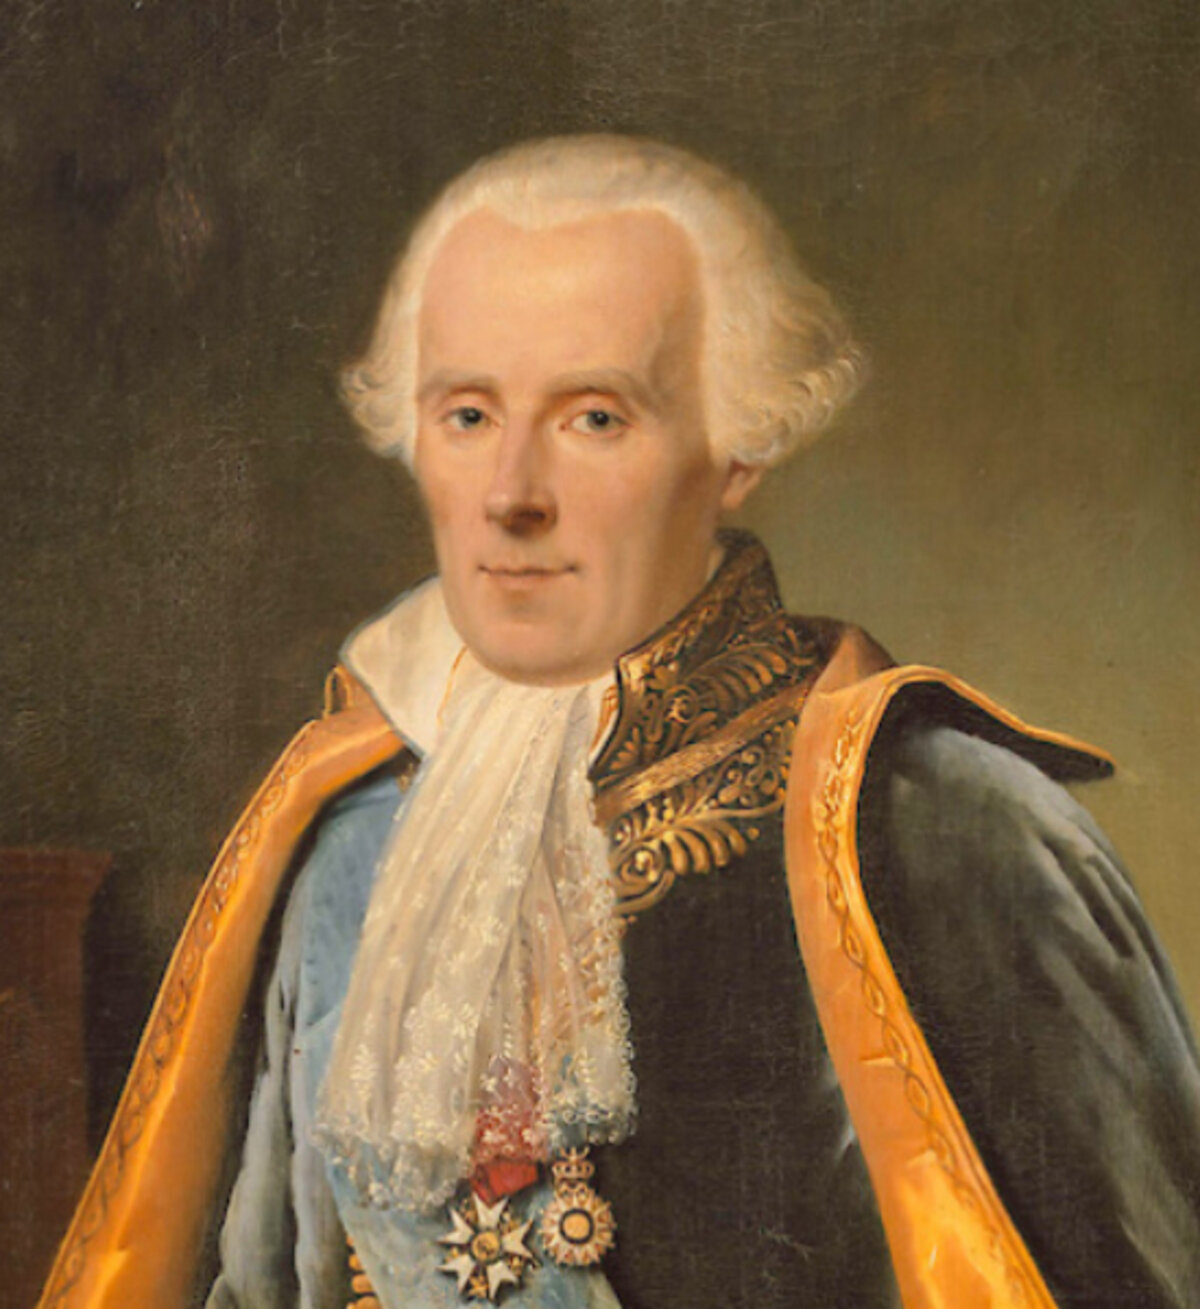
\includegraphics[width=\linewidth,height=0.70\textheight,keepaspectratio]{images-companion/ch08_laplace.jpg}

\caption{Figure C8.3: Pierre-Simon Laplace, Namesake of the Laplace Transform}

\end{figure}

\begin{figure}[H]

\hypertarget{fig-c8-4}{}\label{fig-c8-4}

\centering

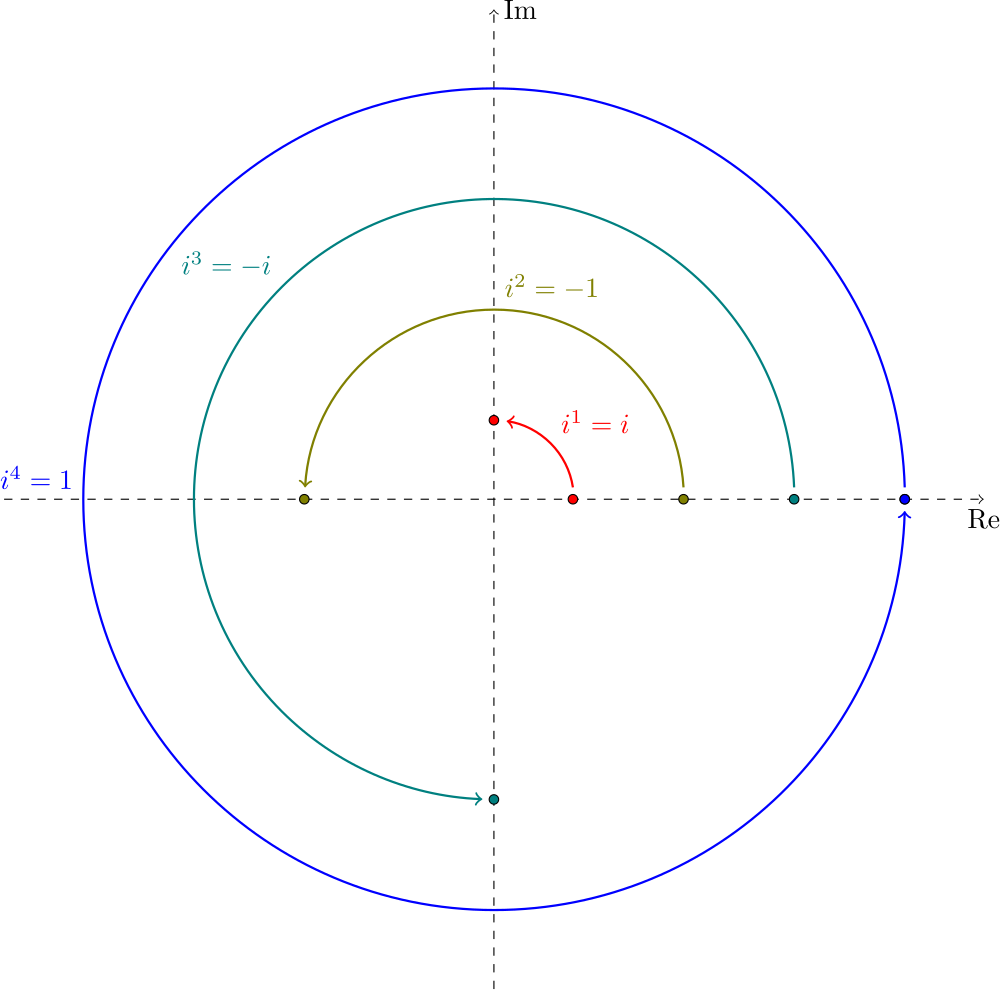
\includegraphics[width=\linewidth,height=0.70\textheight,keepaspectratio]{images-companion/ch08_ztransform.png}

\caption{Figure C8.4: Rotations on the Complex Plane — Basis for the Z-Plane Used in the Z-Transform}

\end{figure}

\begin{figure}[H]

\hypertarget{fig-c8-5}{}\label{fig-c8-5}

\centering

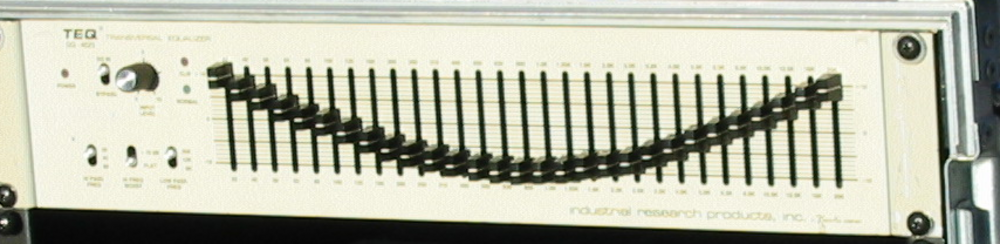
\includegraphics[width=\linewidth,height=0.70\textheight,keepaspectratio]{images-companion/ch08_filters.png}

\caption{Figure C8.5: Graphic Equalizer — a Bank of Adjustable Digital/Analog Filters}

\end{figure}

\begin{figure}[H]

\hypertarget{fig-c8-6}{}\label{fig-c8-6}

\centering

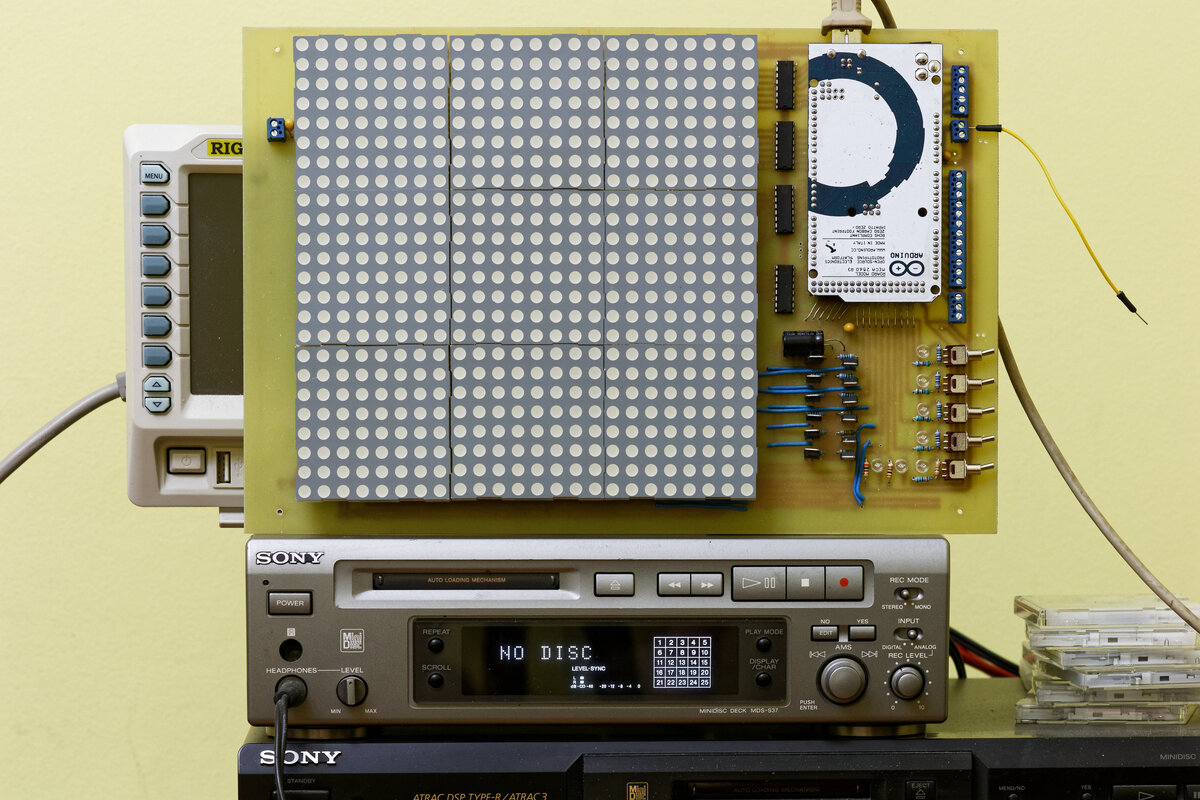
\includegraphics[width=\linewidth,height=0.70\textheight,keepaspectratio]{images-companion/ch08_spectral.jpg}

\caption{Figure C8.6: DIY Arduino-Based LED Audio Spectrum Analyzer}

\end{figure}

\section{Chapter 9: Electromagnetics}\label{chapter-9-electromagnetics}

\begin{figure}[H]

\hypertarget{fig-c9-1}{}\label{fig-c9-1}

\centering

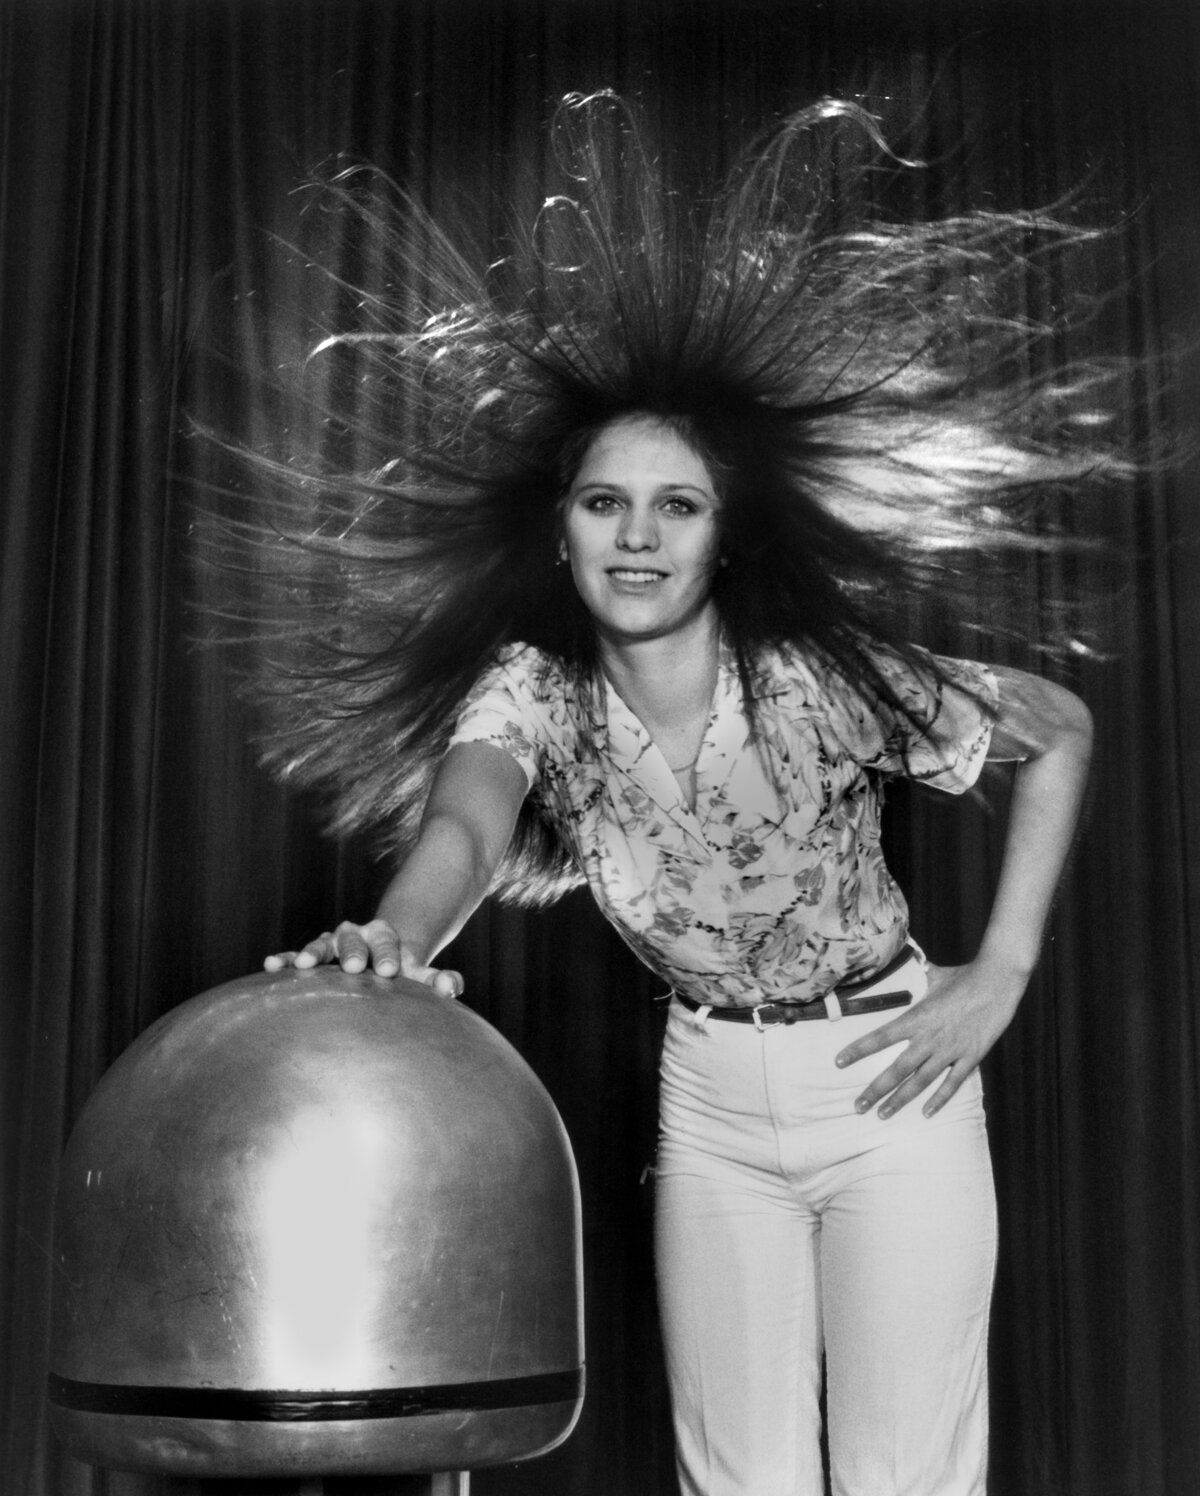
\includegraphics[width=\linewidth,height=0.70\textheight,keepaspectratio]{images-companion/ch09_electrostatics.jpg}

\caption{Figure C9.1: Van de Graaff Generator — Electrostatic Charge Demonstration}

\end{figure}

\begin{figure}[H]

\hypertarget{fig-c9-2}{}\label{fig-c9-2}

\centering

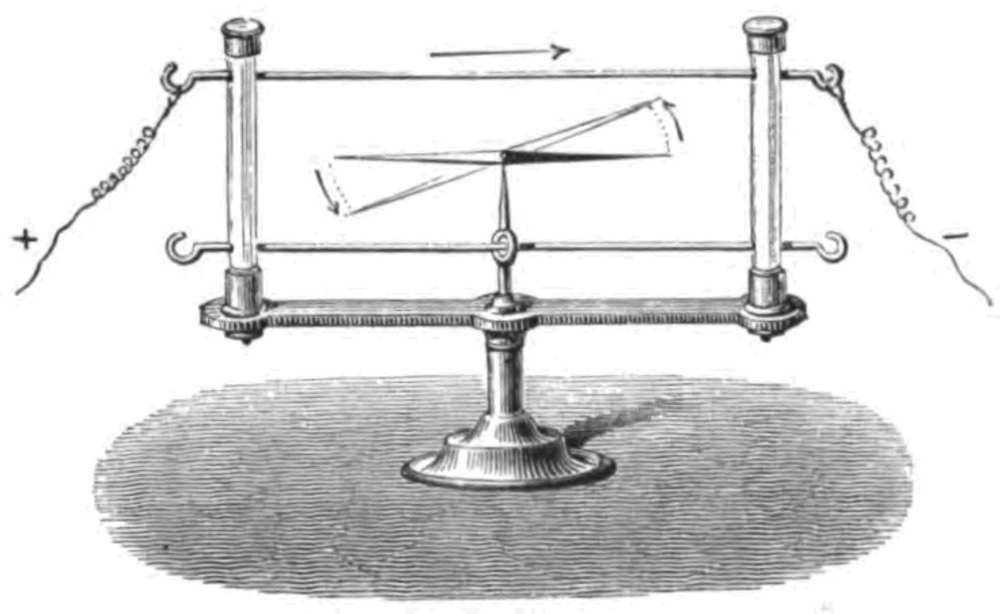
\includegraphics[width=\linewidth,height=0.70\textheight,keepaspectratio]{images-companion/ch09_magnetostatics.png}

\caption{Figure C9.2: Ørsted’s Experiment — Current-Carrying Wire Deflecting a Compass Needle}

\end{figure}

\begin{figure}[H]

\hypertarget{fig-c9-3}{}\label{fig-c9-3}

\centering

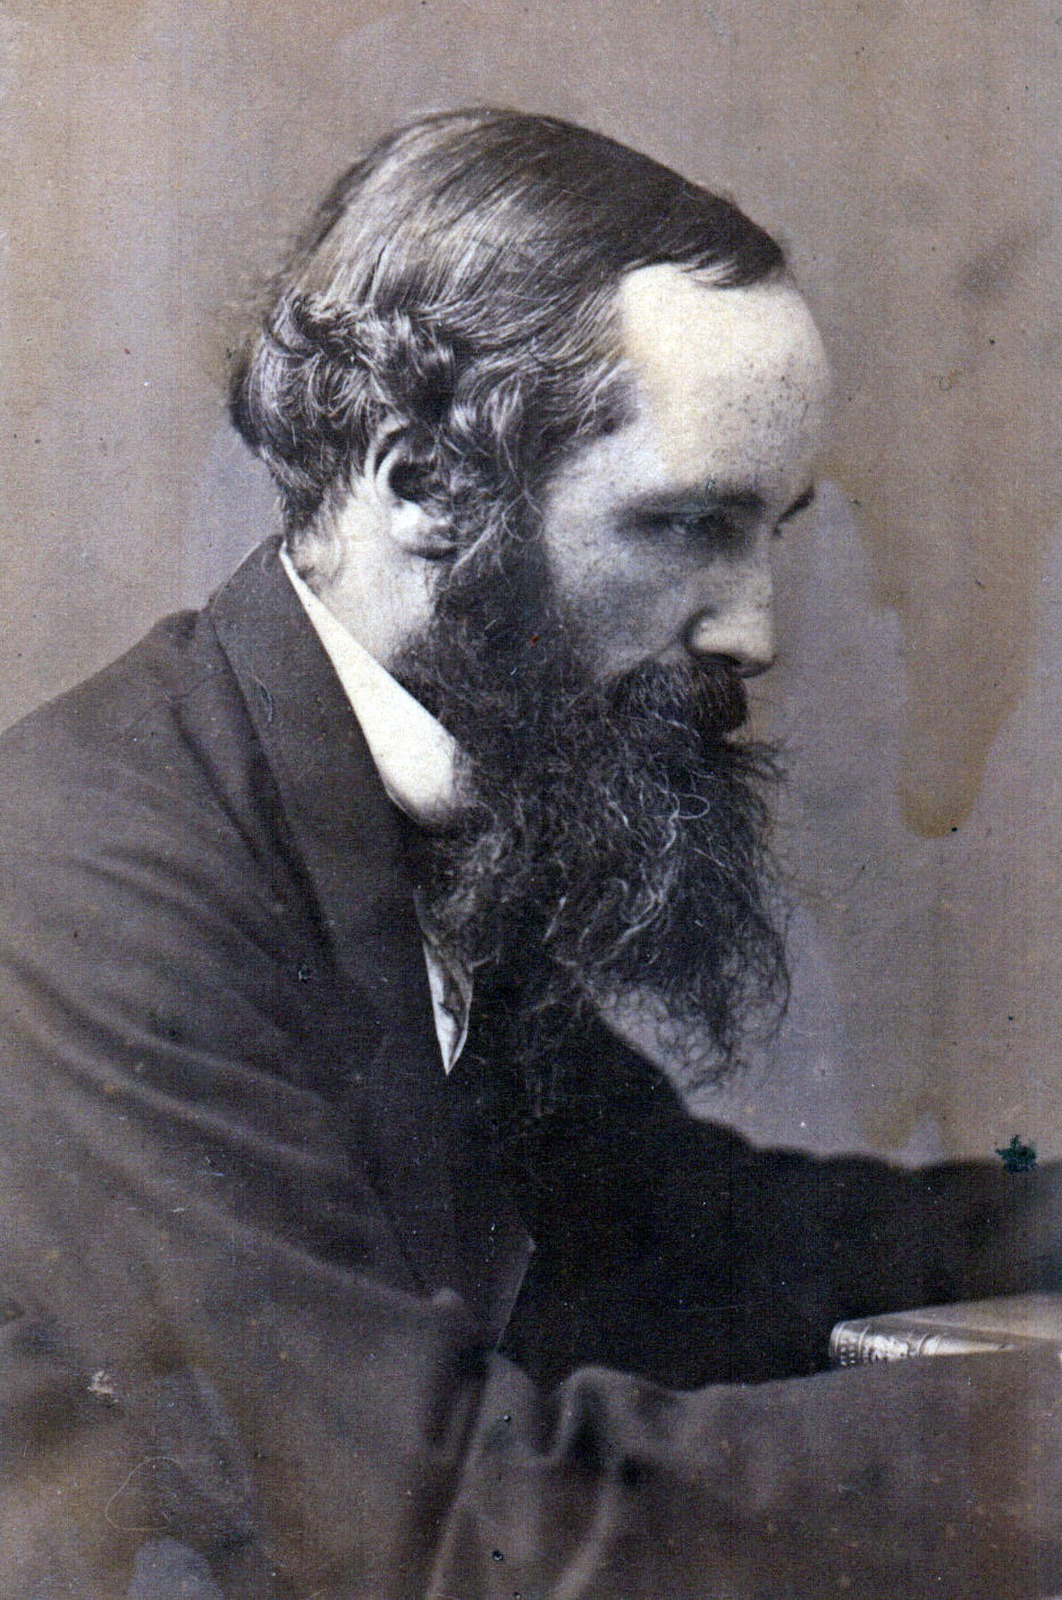
\includegraphics[width=\linewidth,height=0.70\textheight,keepaspectratio]{images-companion/ch09_maxwell.jpg}

\caption{Figure C9.3: James Clerk Maxwell, Formulator of Maxwell’s Equations}

\end{figure}

\begin{figure}[H]

\hypertarget{fig-c9-4}{}\label{fig-c9-4}

\centering

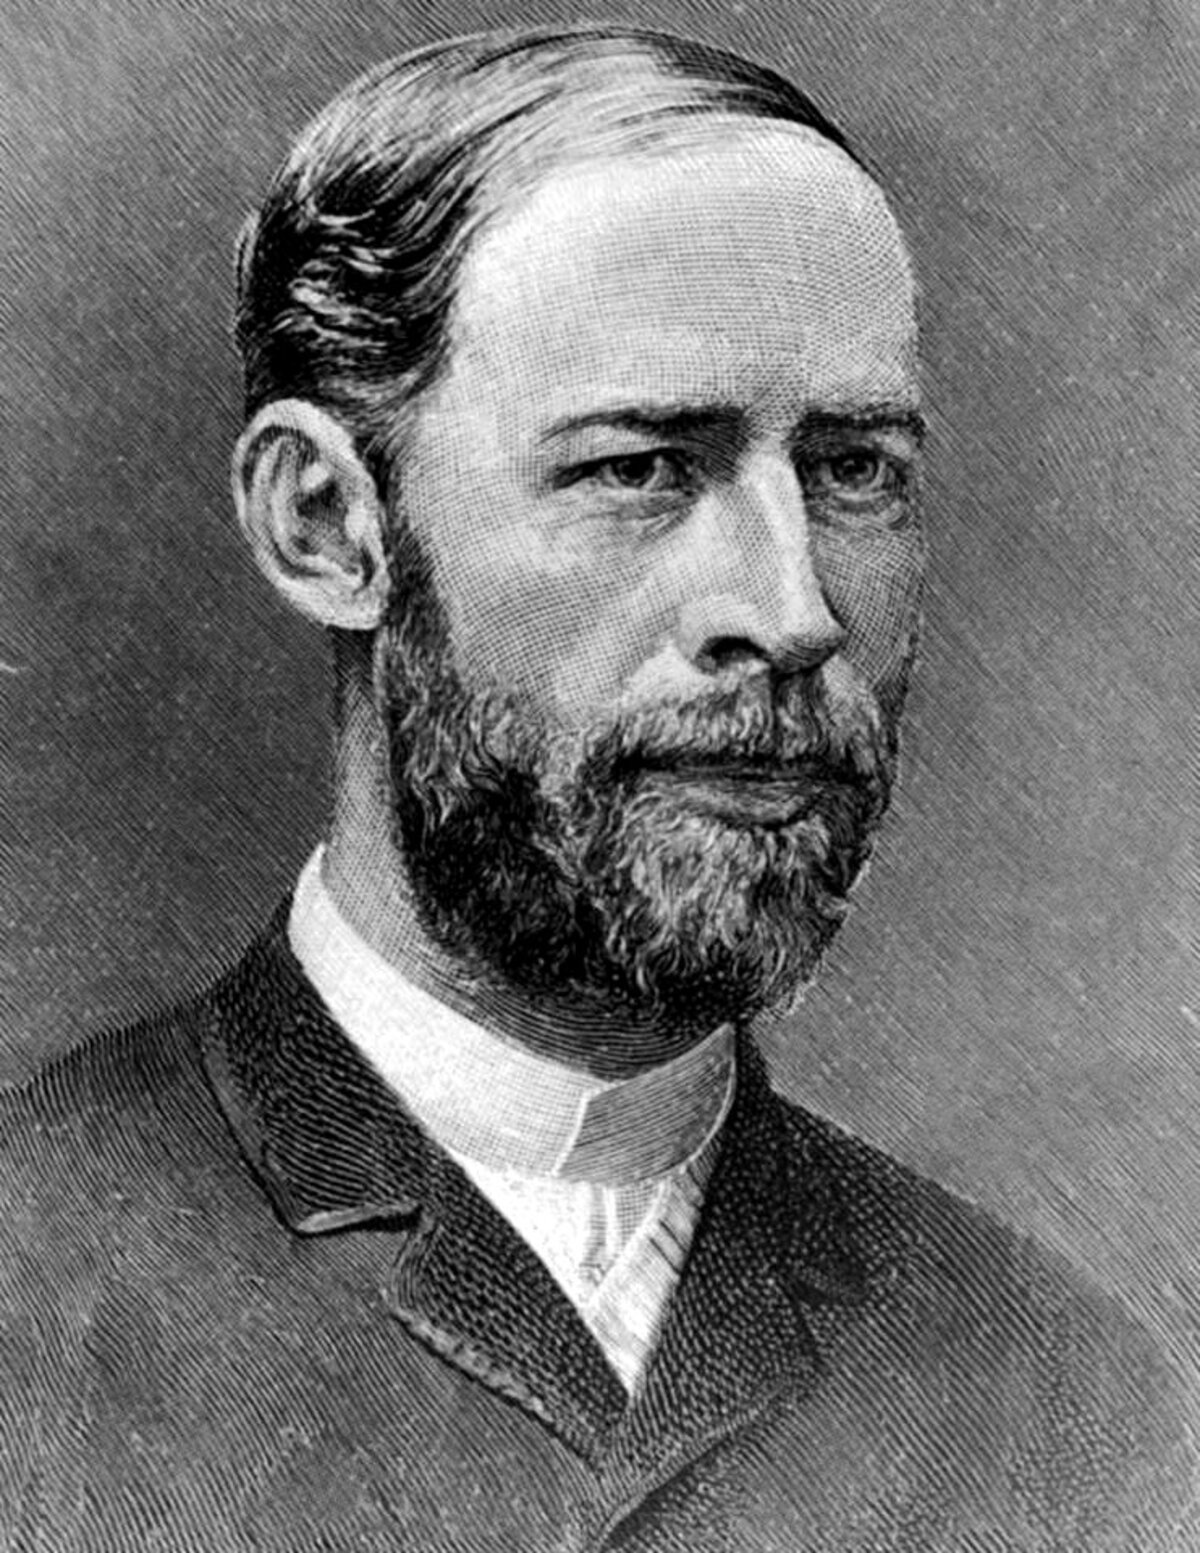
\includegraphics[width=\linewidth,height=0.70\textheight,keepaspectratio]{images-companion/ch09_hertz.jpg}

\caption{Figure C9.4: Heinrich Hertz, First to Demonstrate Electromagnetic Waves}

\end{figure}

\begin{figure}[H]

\hypertarget{fig-c9-5}{}\label{fig-c9-5}

\centering

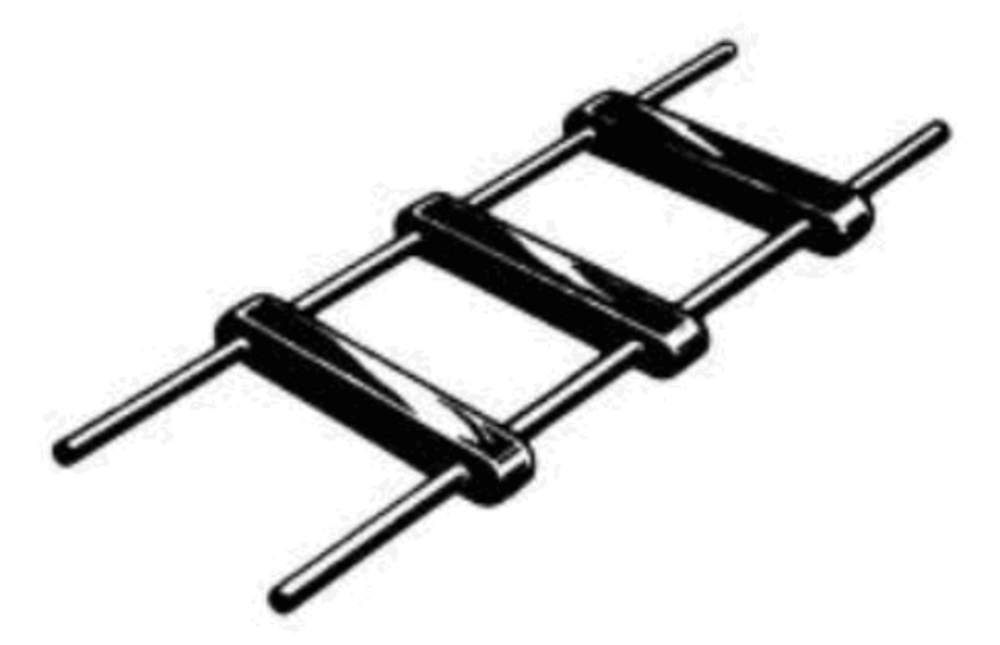
\includegraphics[width=\linewidth,height=0.70\textheight,keepaspectratio]{images-companion/ch09_translines.png}

\caption{Figure C9.5: Ladder Line — an Open-Wire Balanced Transmission Line}

\end{figure}

\begin{figure}[H]

\hypertarget{fig-c9-6}{}\label{fig-c9-6}

\centering

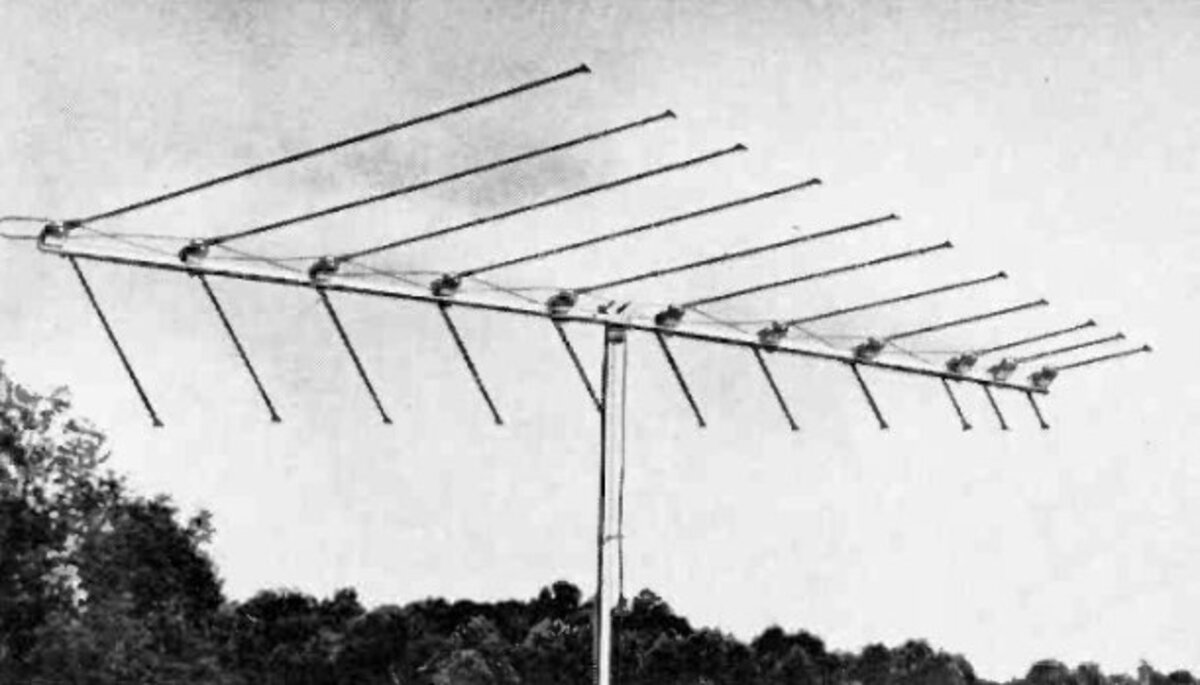
\includegraphics[width=\linewidth,height=0.70\textheight,keepaspectratio]{images-companion/ch09_antennas.jpg}

\caption{Figure C9.6: Log-Periodic VHF TV Antenna (1963)}

\end{figure}

\section{Chapter 10: Power
Electronics}\label{chapter-10-power-electronics}

\begin{figure}[H]

\hypertarget{fig-c10-2}{}\label{fig-c10-2}

\centering

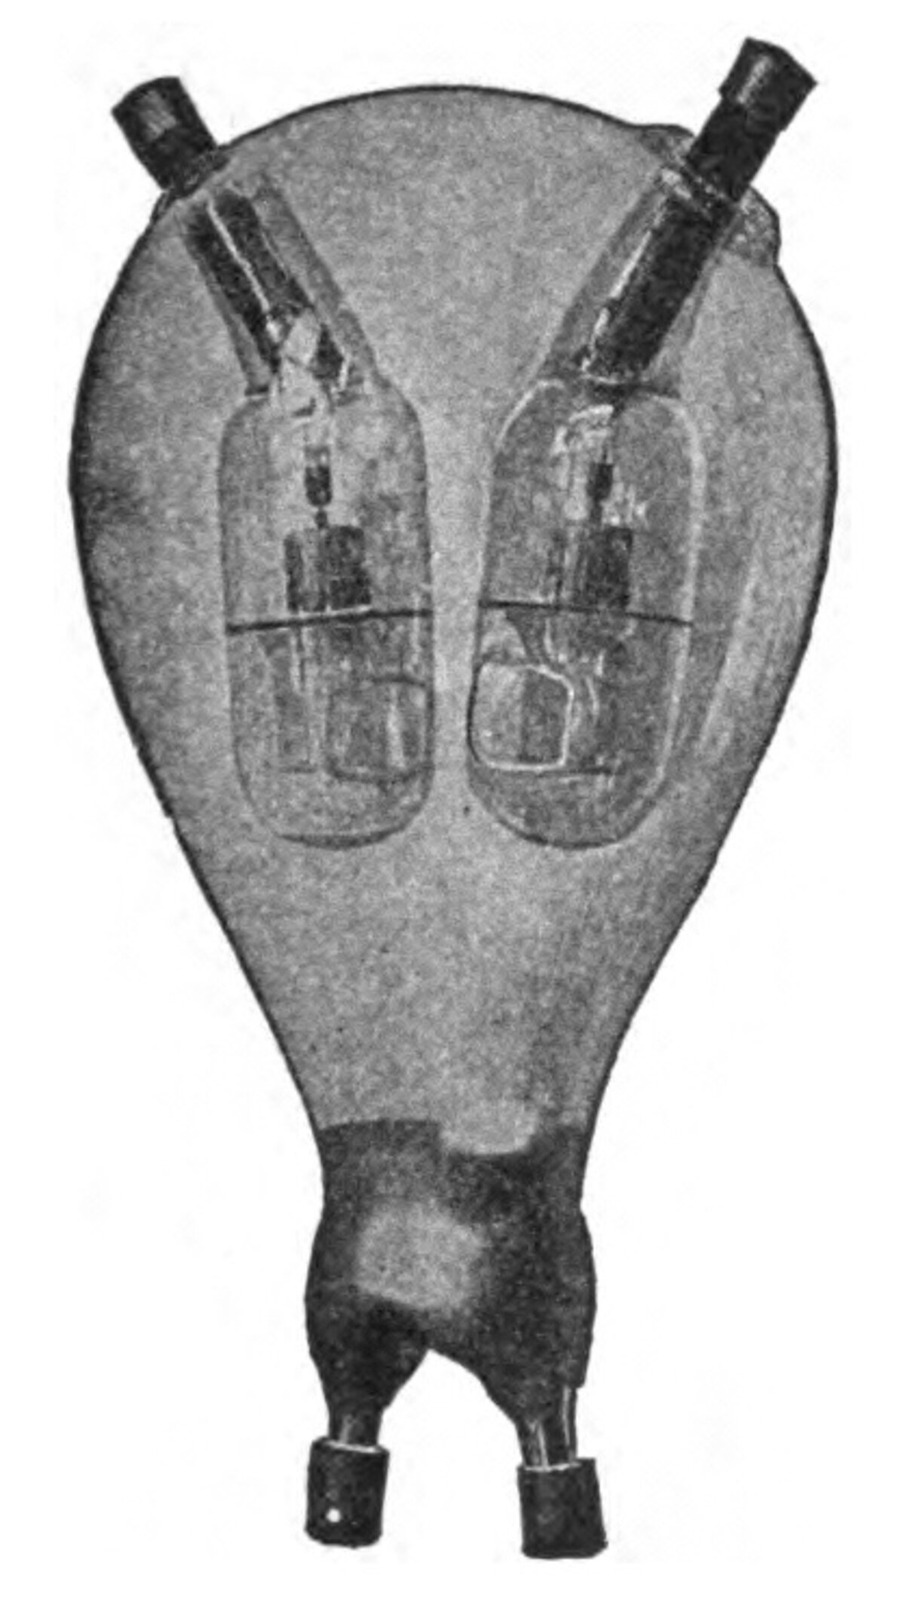
\includegraphics[width=\linewidth,height=0.70\textheight,keepaspectratio]{images-companion/ch10_rectifiers.jpg}

\caption{Figure C10.2: Twin-Anode Mercury-Arc Rectifier Bulb}

\end{figure}

\begin{figure}[H]

\hypertarget{fig-c10-3}{}\label{fig-c10-3}

\centering

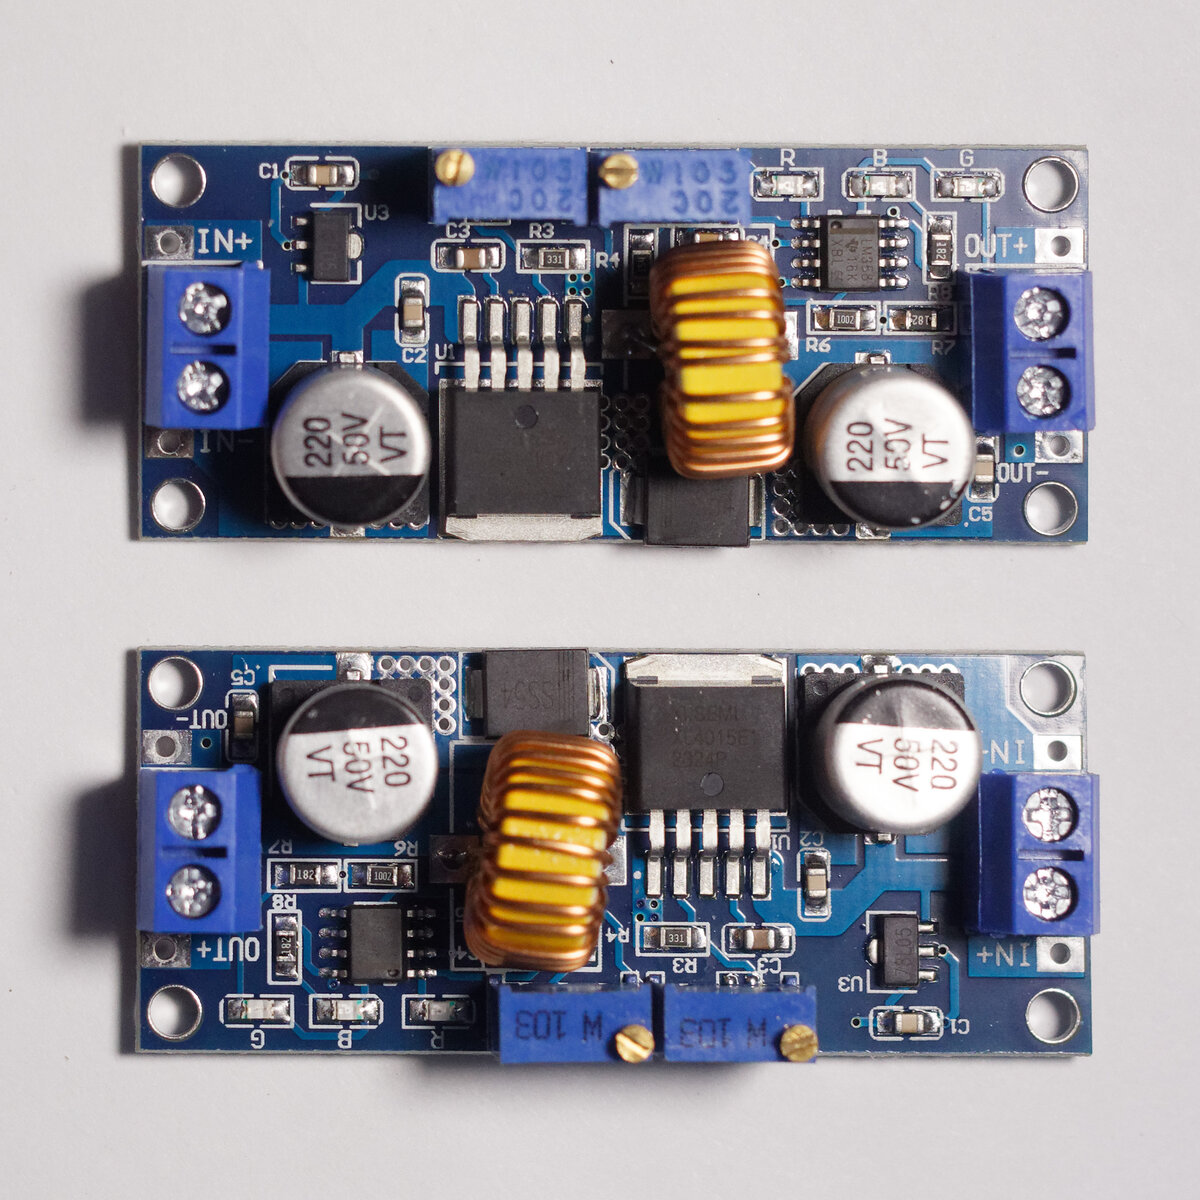
\includegraphics[width=\linewidth,height=0.70\textheight,keepaspectratio]{images-companion/ch10_dcdc.jpg}

\caption{Figure C10.3: XL4015-Based CC/CV Buck Converter Modules}

\end{figure}

\begin{figure}[H]

\hypertarget{fig-c10-5}{}\label{fig-c10-5}

\centering

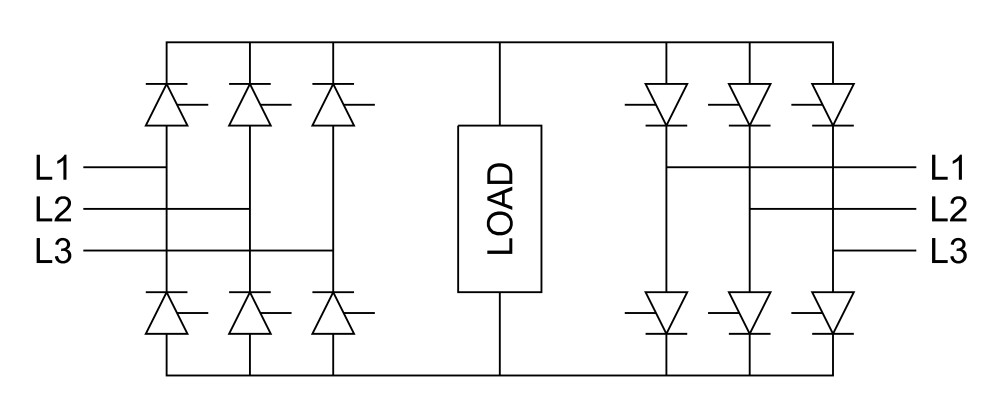
\includegraphics[width=\linewidth,height=0.70\textheight,keepaspectratio]{images-companion/ch10_acac.png}

\caption{Figure C10.5: Cycloconverter Circuit Diagram (Direct AC-AC Conversion)}

\end{figure}

\begin{figure}[H]

\hypertarget{fig-c10-6}{}\label{fig-c10-6}

\centering

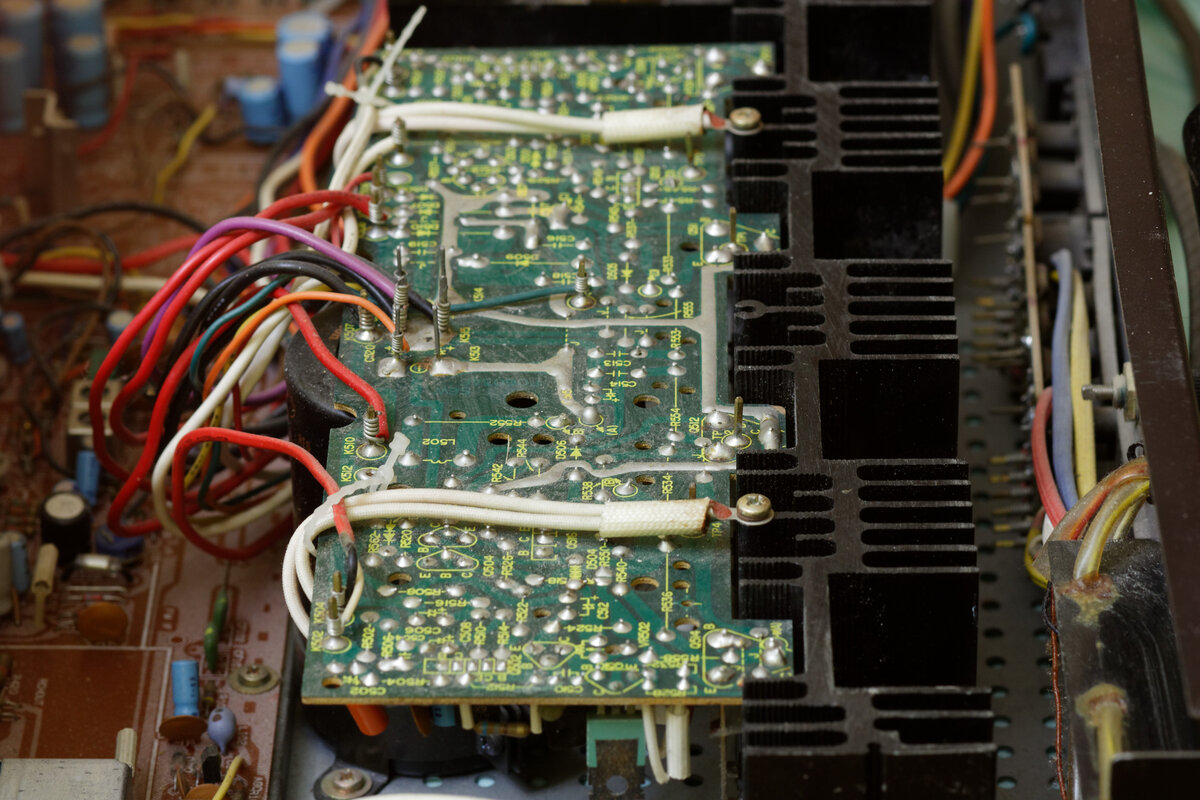
\includegraphics[width=\linewidth,height=0.70\textheight,keepaspectratio]{images-companion/ch10_thermal.jpg}

\caption{Figure C10.6: Heatsinked Power Amplifier Output Transistors — Thermal Management in Power Electronics}

\end{figure}

\begin{figure}[H]

\hypertarget{fig-c10-7}{}\label{fig-c10-7}

\centering

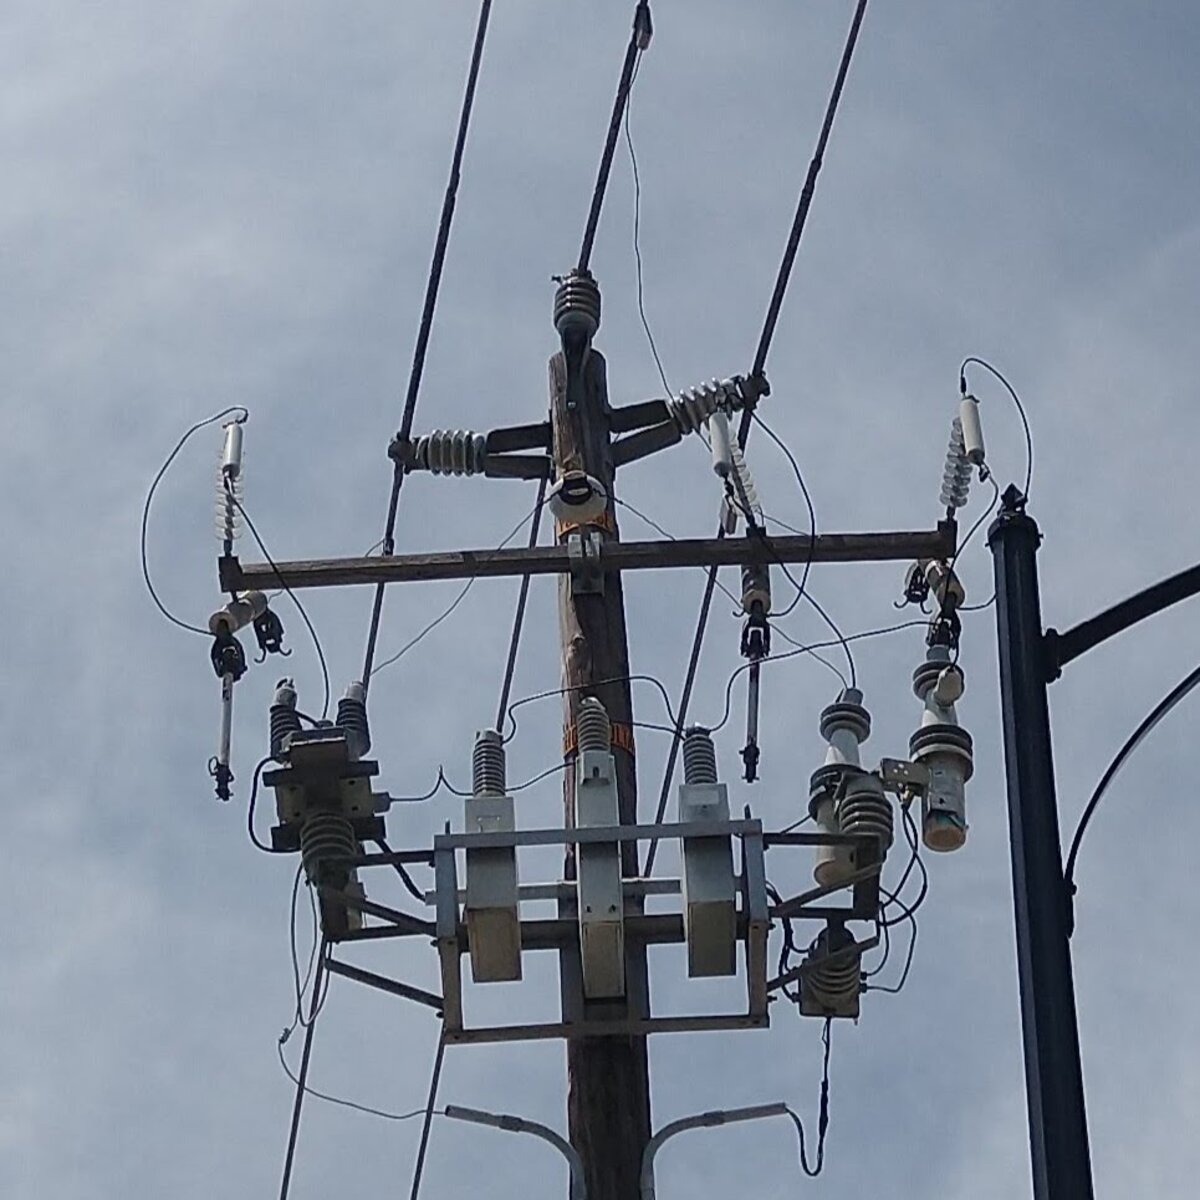
\includegraphics[width=\linewidth,height=0.70\textheight,keepaspectratio]{images-companion/ch10_pfc.jpg}

\caption{Figure C10.7: Pole-Mounted Power Factor Correction Capacitor Bank}

\end{figure}

\begin{figure}[H]

\hypertarget{fig-c10-8}{}\label{fig-c10-8}

\centering

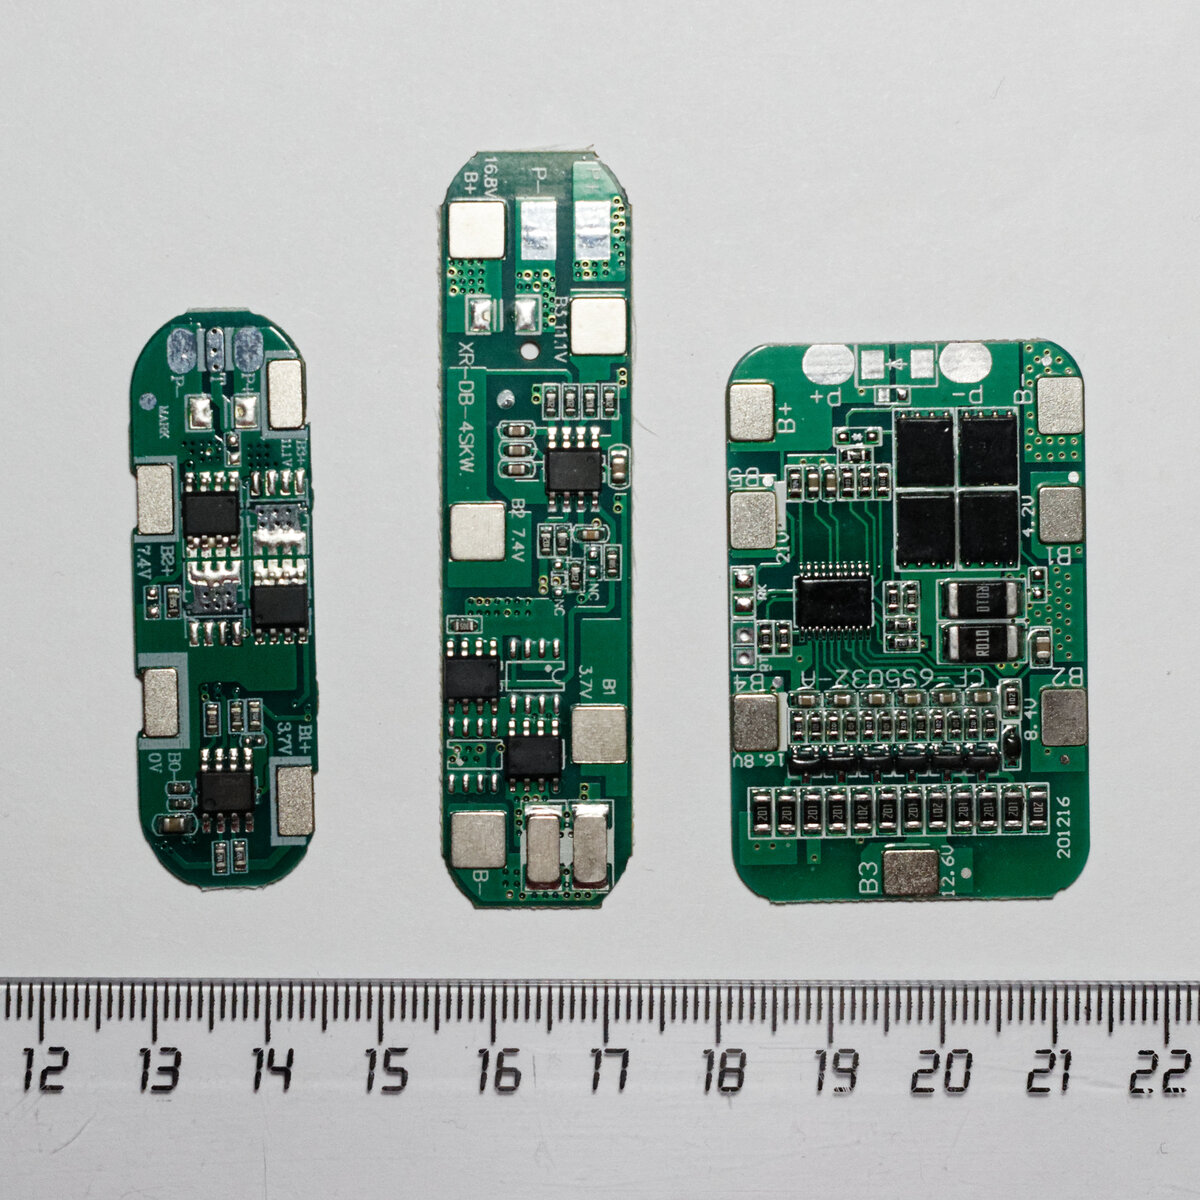
\includegraphics[width=\linewidth,height=0.70\textheight,keepaspectratio]{images-companion/ch10_bms.jpg}

\caption{Figure C10.8: Generic Lithium Battery Management System (BMS) Boards, 3S/4S/6S}

\end{figure}

\begin{figure}[H]

\hypertarget{fig-c10-10}{}\label{fig-c10-10}

\centering

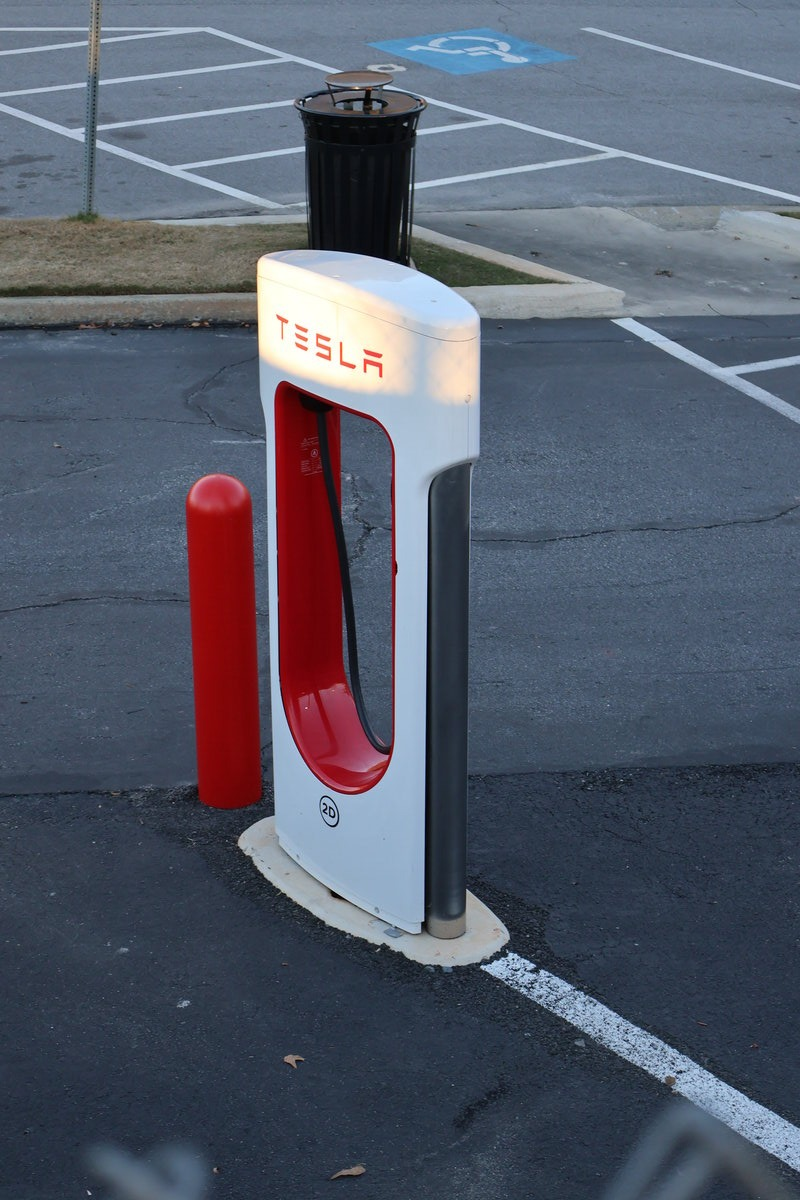
\includegraphics[width=\linewidth,height=0.70\textheight,keepaspectratio]{images-companion/ch10_charging.jpg}

\caption{Figure C10.10: Tesla V3 Supercharger — High-Power DC Fast Charging Station}

\end{figure}

\begin{figure}[H]

\hypertarget{fig-c10-11}{}\label{fig-c10-11}

\centering

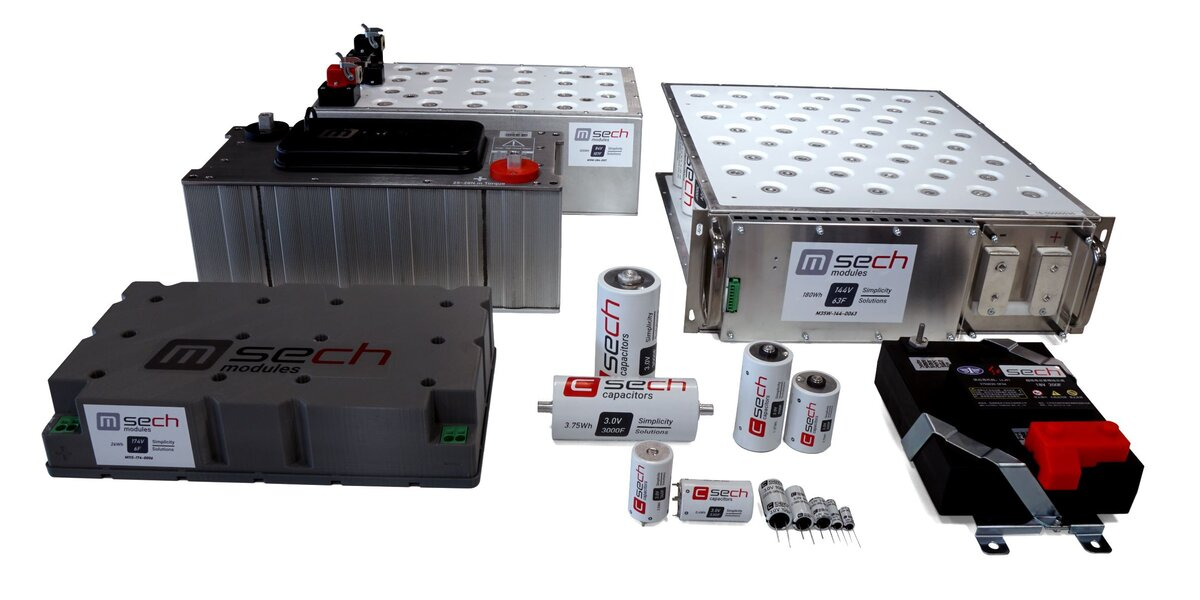
\includegraphics[width=\linewidth,height=0.70\textheight,keepaspectratio]{images-companion/ch10_supercap.jpg}

\caption{Figure C10.11: Commercial Supercapacitor (Ultracapacitor) Products}

\end{figure}

\begin{figure}[H]

\hypertarget{fig-c10-12}{}\label{fig-c10-12}

\centering

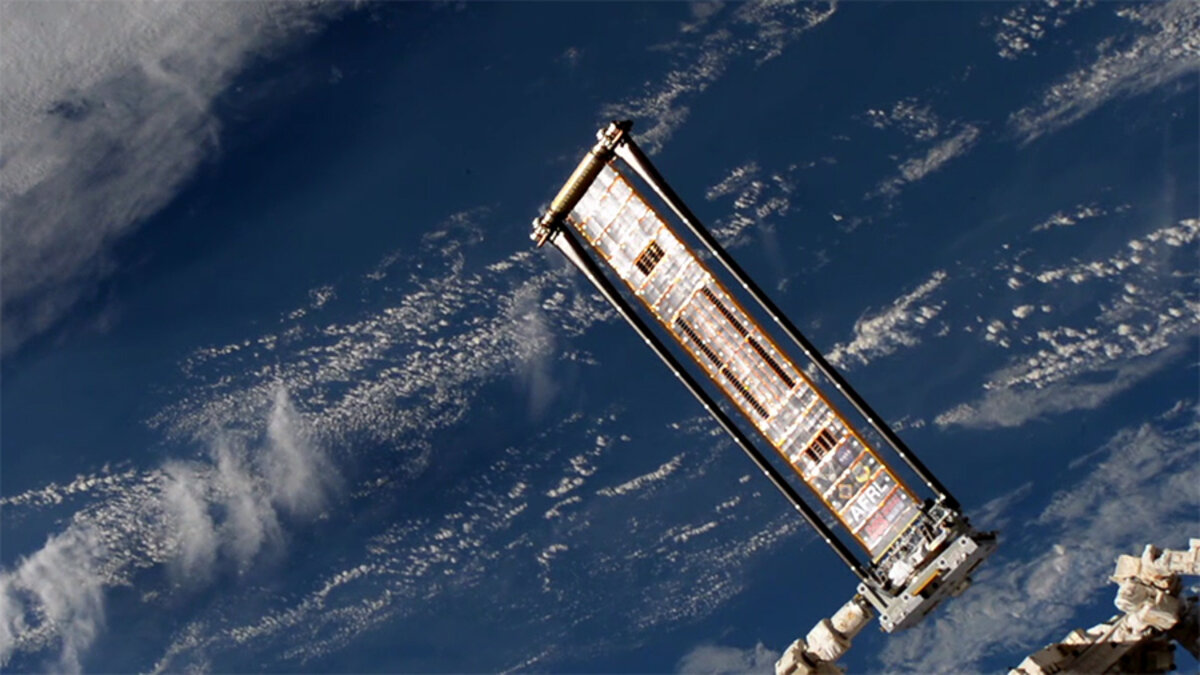
\includegraphics[width=\linewidth,height=0.70\textheight,keepaspectratio]{images-companion/ch10_solarpv.jpg}

\caption{Figure C10.12: Roll-Out Solar Array (ROSA) Deployed on the International Space Station}

\end{figure}

\section{Chapter 11: Instrumentation and
Measurement}\label{chapter-11-instrumentation-and-measurement}

\begin{figure}[H]

\hypertarget{fig-c11-2}{}\label{fig-c11-2}

\centering

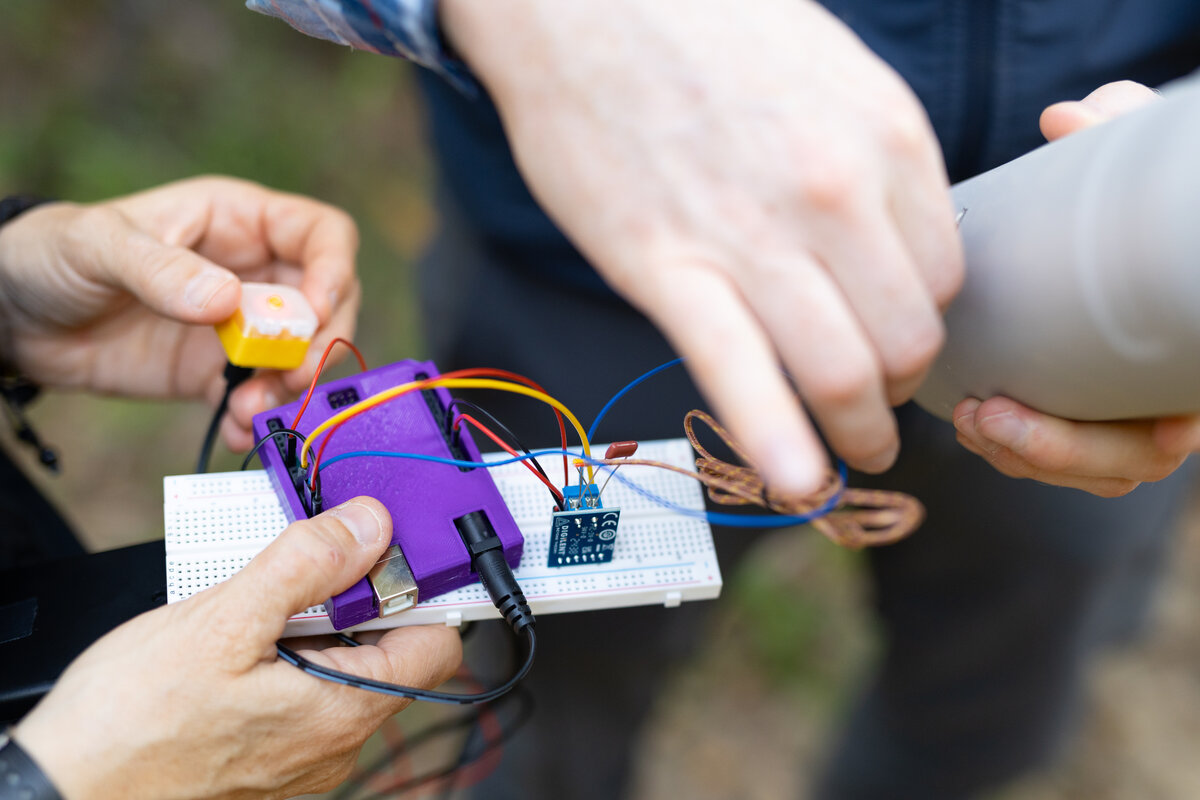
\includegraphics[width=\linewidth,height=0.70\textheight,keepaspectratio]{images-companion/ch11_sensors.jpg}

\caption{Figure C11.2: Breadboarded Sensor Module with Digital Readout — Field Data Collection}

\end{figure}

\begin{figure}[H]

\hypertarget{fig-c11-4}{}\label{fig-c11-4}

\centering

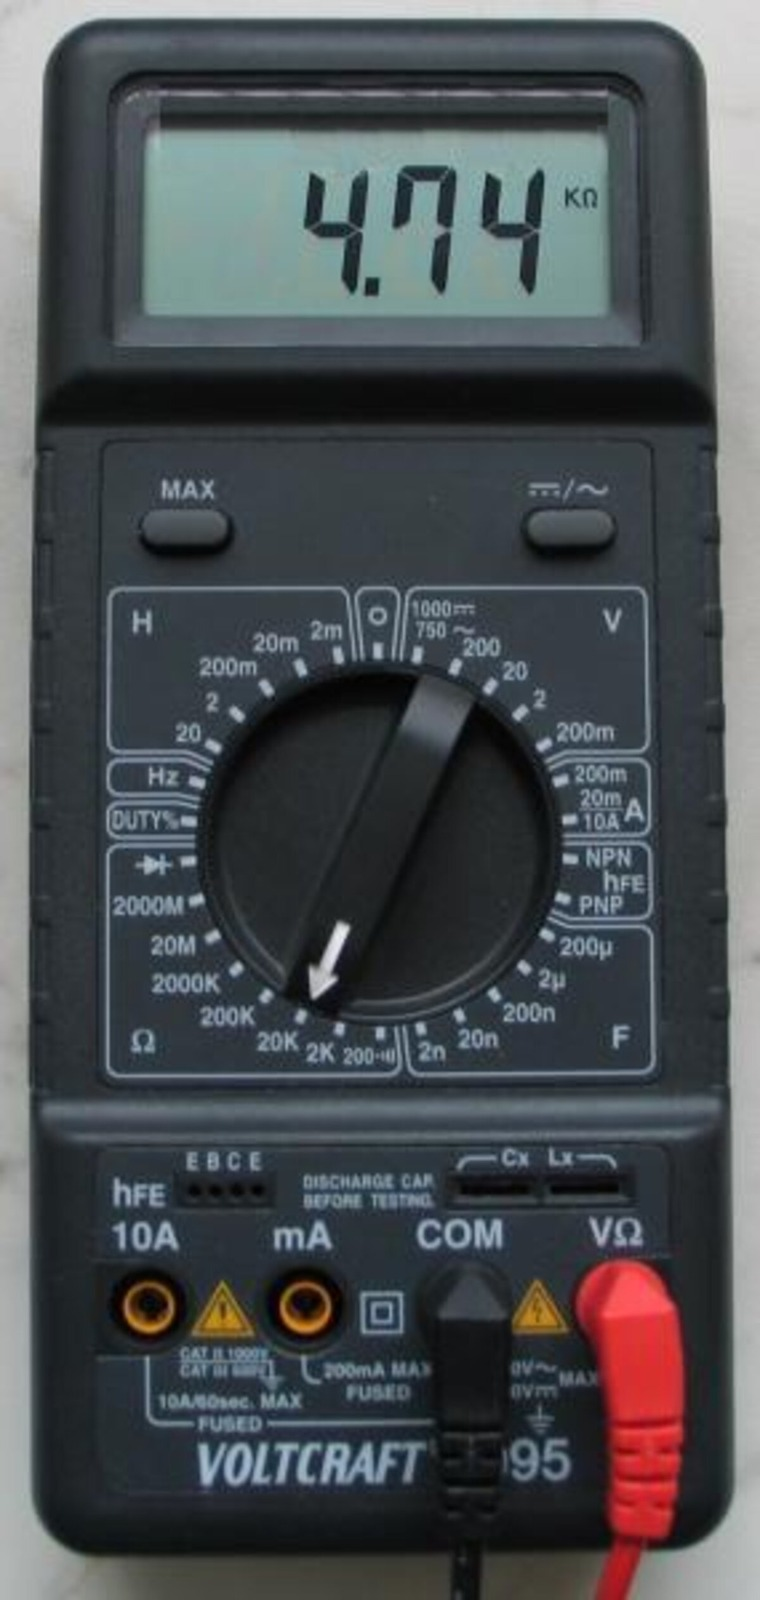
\includegraphics[width=\linewidth,height=0.70\textheight,keepaspectratio]{images-companion/ch11_instruments.jpg}

\caption{Figure C11.4: Handheld Digital Multimeter — a Common Measurement Instrument}

\end{figure}

\begin{figure}[H]

\hypertarget{fig-c11-5}{}\label{fig-c11-5}

\centering

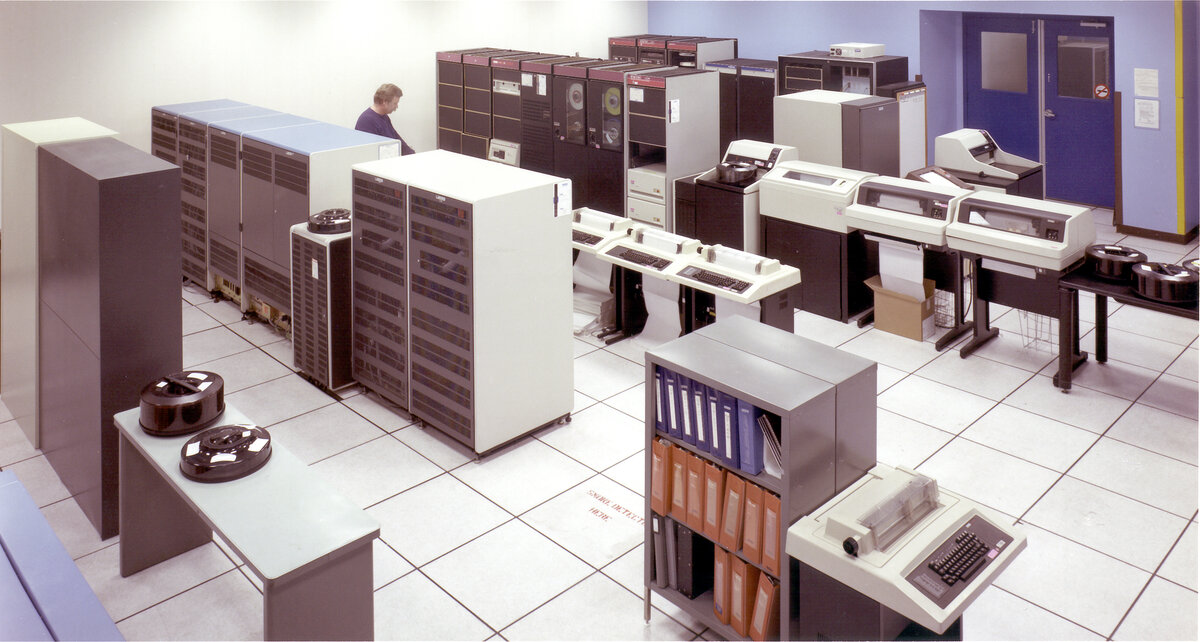
\includegraphics[width=\linewidth,height=0.70\textheight,keepaspectratio]{images-companion/ch11_daq.jpg}

\caption{Figure C11.5: Wind-Tunnel Data Acquisition System Computer Room}

\end{figure}

\section{Chapter 12: Electric Motors}\label{chapter-12-electric-motors}

\begin{figure}[H]

\hypertarget{fig-c12-1}{}\label{fig-c12-1}

\centering

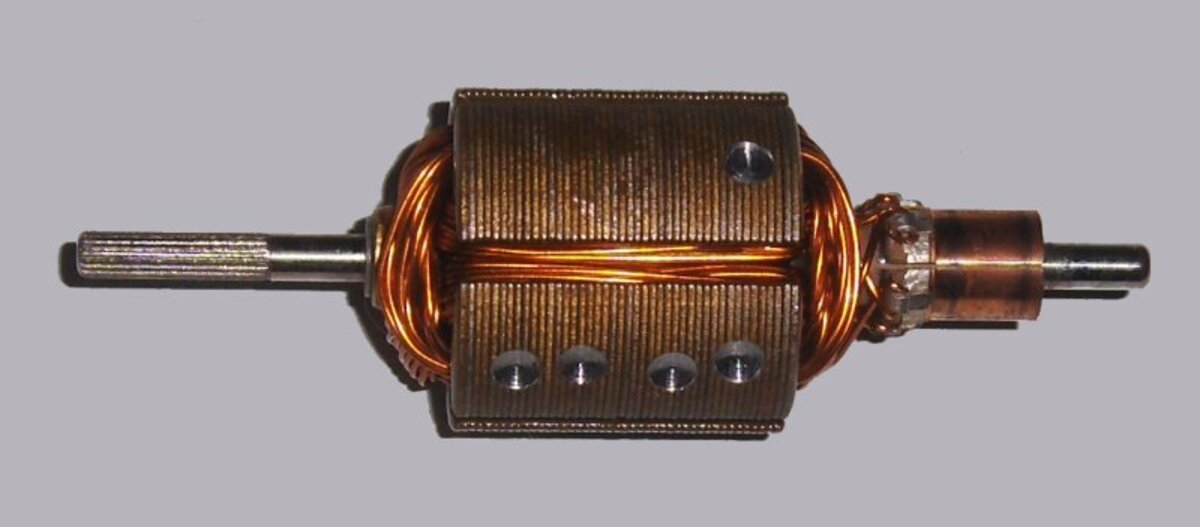
\includegraphics[width=\linewidth,height=0.70\textheight,keepaspectratio]{images-companion/ch12_dcmotors.jpg}

\caption{Figure C12.1: DC Motor Armature with Commutator and Windings}

\end{figure}

\begin{figure}[H]

\hypertarget{fig-c12-2}{}\label{fig-c12-2}

\centering

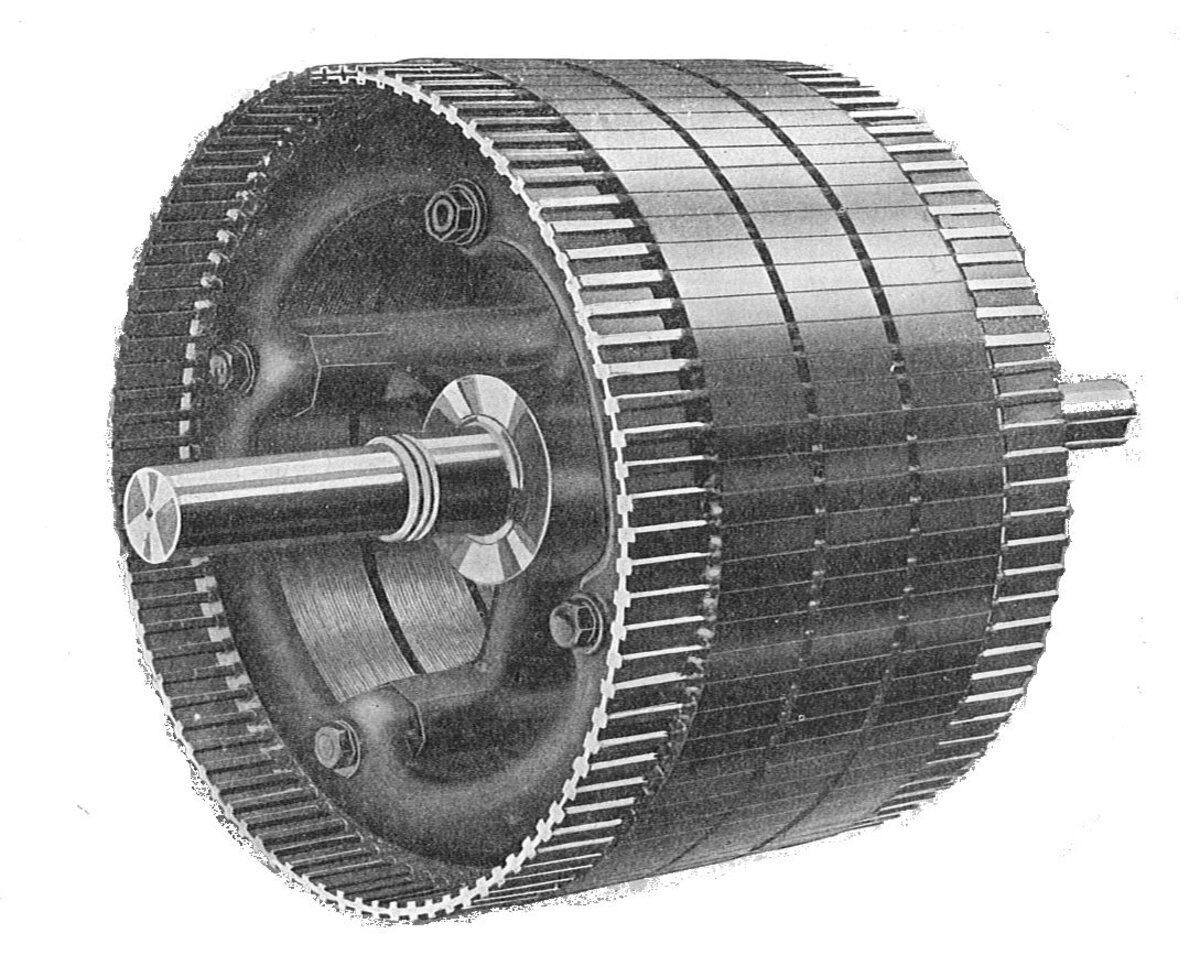
\includegraphics[width=\linewidth,height=0.70\textheight,keepaspectratio]{images-companion/ch12_acmotors.jpg}

\caption{Figure C12.2: Squirrel-Cage Induction Motor Rotor (1909)}

\end{figure}

\section{Chapter 13: Operational
Amplifiers}\label{chapter-13-operational-amplifiers}

\begin{figure}[H]

\hypertarget{fig-c13-1}{}\label{fig-c13-1}

\centering

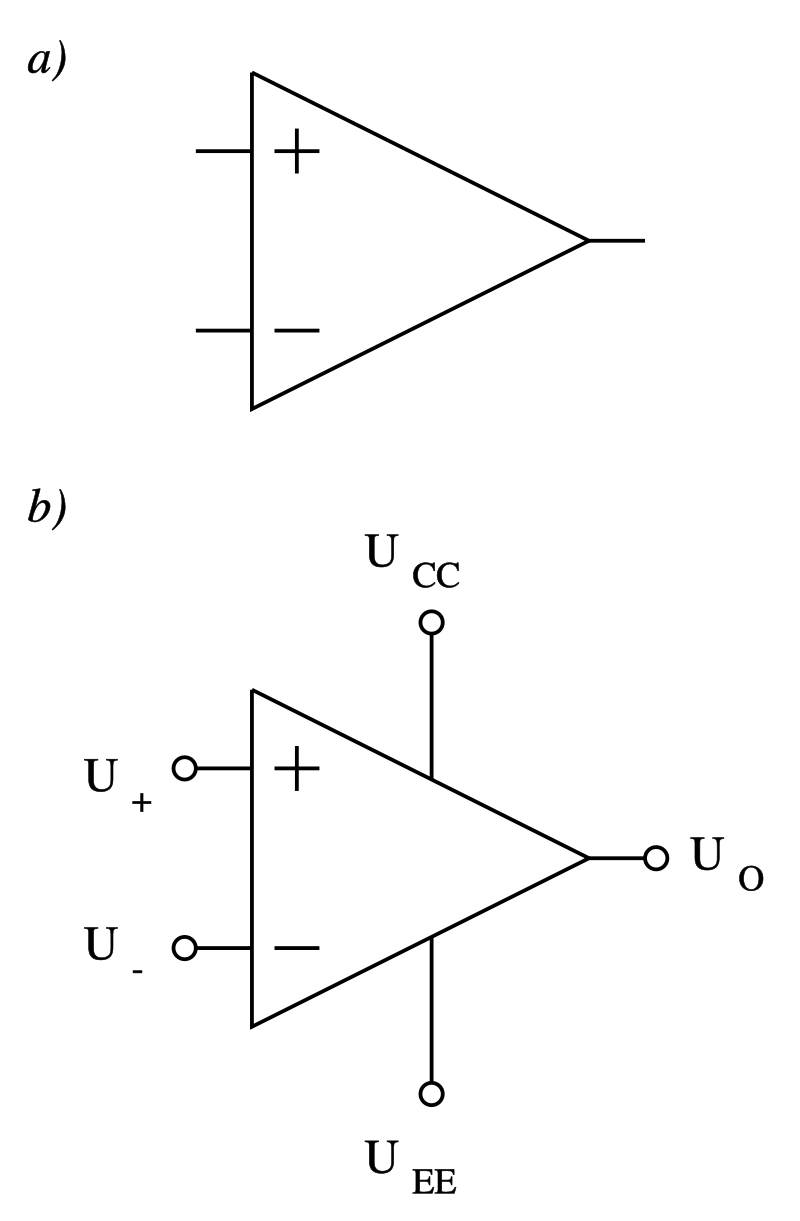
\includegraphics[width=\linewidth,height=0.70\textheight,keepaspectratio]{images-companion/ch13_ideal.png}

\caption{Figure C13.1: Ideal Op-Amp Symbol, With and Without Supply Rails Shown}

\end{figure}

\begin{figure}[H]

\hypertarget{fig-c13-2}{}\label{fig-c13-2}

\centering

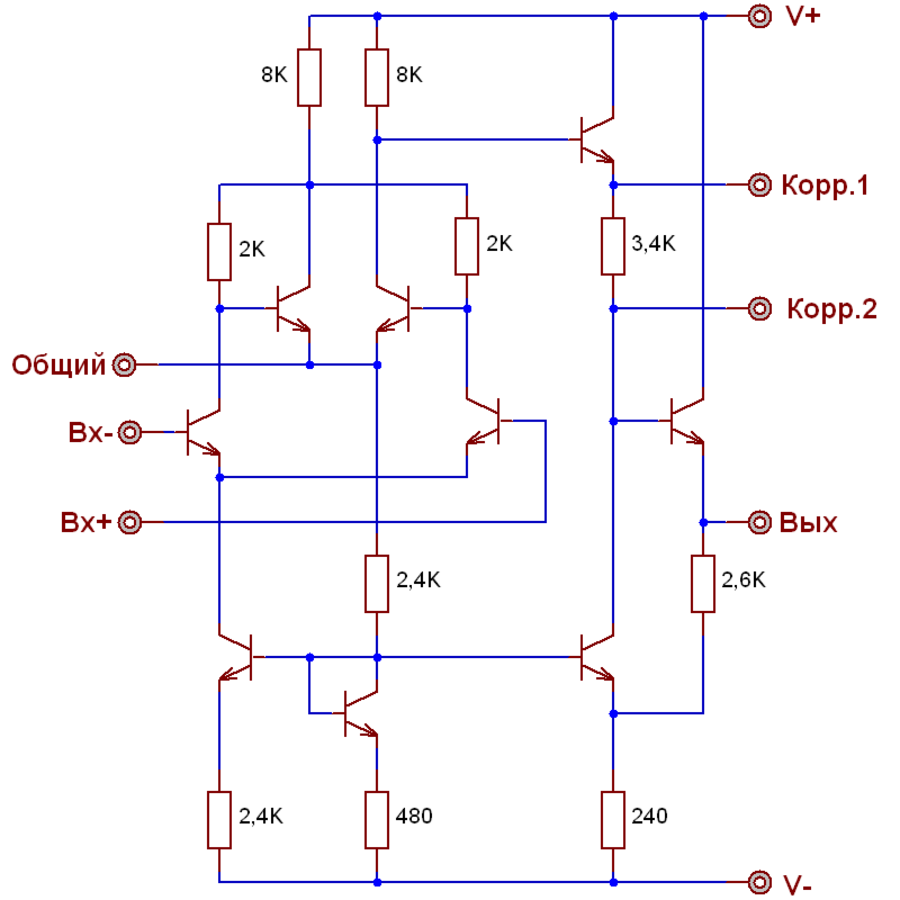
\includegraphics[width=\linewidth,height=0.70\textheight,keepaspectratio]{images-companion/ch13_inverting.png}

\caption{Figure C13.2: Internal Transistor-Level Schematic of the μA702, the First Monolithic Op-Amp (Bob Widlar, 1964)}

\end{figure}

\begin{figure}[H]

\hypertarget{fig-c13-4}{}\label{fig-c13-4}

\centering

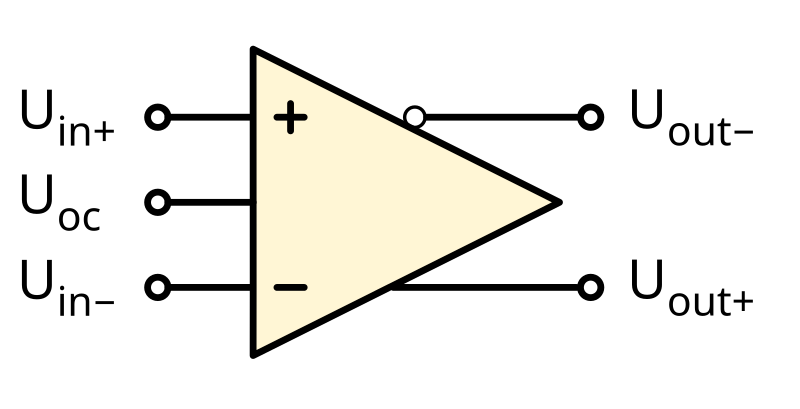
\includegraphics[width=\linewidth,height=0.70\textheight,keepaspectratio]{images-companion/ch13_diffamp.png}

\caption{Figure C13.4: Fully-Differential Amplifier Symbol}

\end{figure}

\begin{figure}[H]

\hypertarget{fig-c13-6}{}\label{fig-c13-6}

\centering

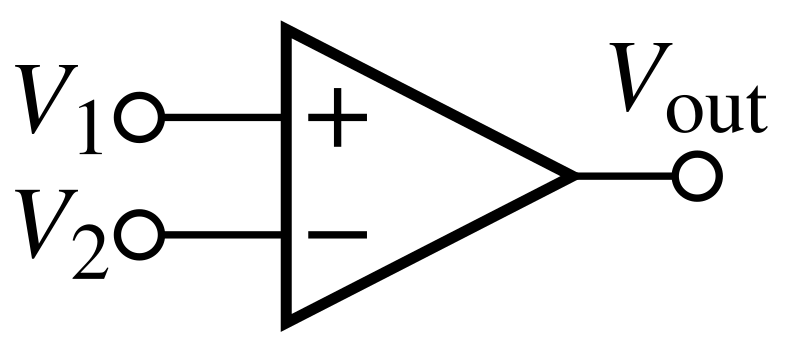
\includegraphics[width=\linewidth,height=0.70\textheight,keepaspectratio]{images-companion/ch13_comparator.png}

\caption{Figure C13.6: Op-Amp Used as a Comparator — Symbol and Convention}

\end{figure}

\section{Chapter 14: National Electrical Code
(NEC)}\label{chapter-14-national-electrical-code-nec}

\begin{figure}[H]

\hypertarget{fig-c14-2}{}\label{fig-c14-2}

\centering

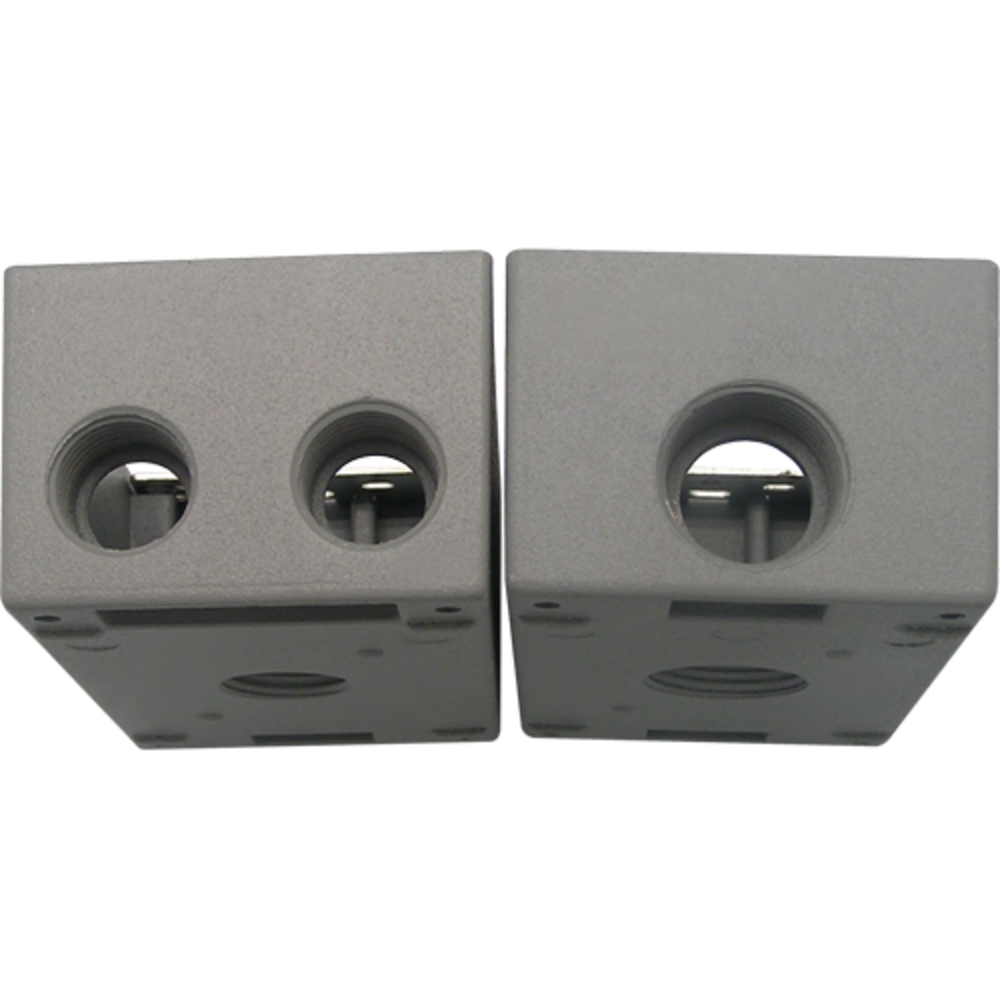
\includegraphics[width=\linewidth,height=0.70\textheight,keepaspectratio]{images-companion/ch14_conductorsizing.png}

\caption{Figure C14.2: Weatherproof Electrical Device Box for Conductor Terminations}

\end{figure}

\begin{figure}[H]

\hypertarget{fig-c14-6}{}\label{fig-c14-6}

\centering

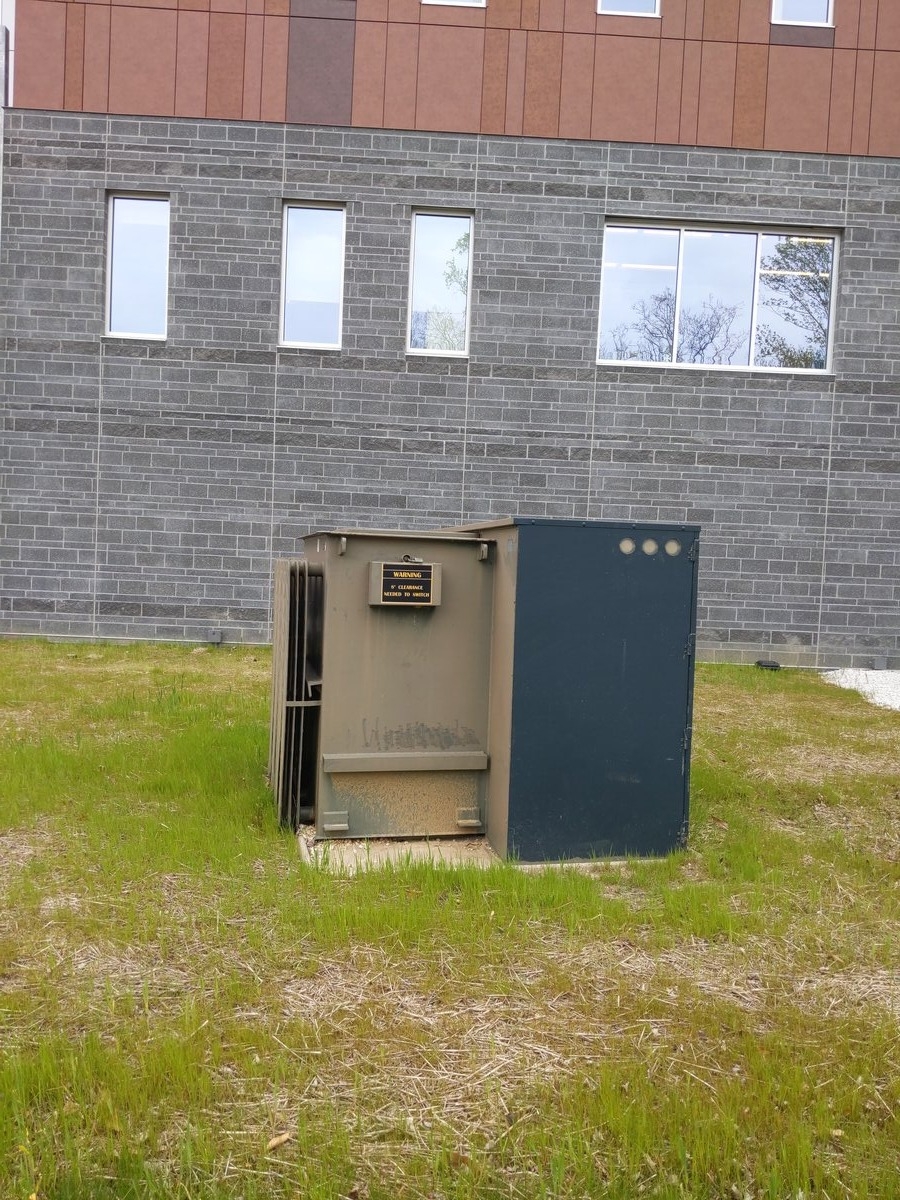
\includegraphics[width=\linewidth,height=0.70\textheight,keepaspectratio]{images-companion/ch14_transformers.jpg}

\caption{Figure C14.6: Pad-Mounted Distribution Transformer}

\end{figure}

\section{Chapter 15: Networking}\label{chapter-15-networking}

\begin{figure}[H]

\hypertarget{fig-c15-1}{}\label{fig-c15-1}

\centering

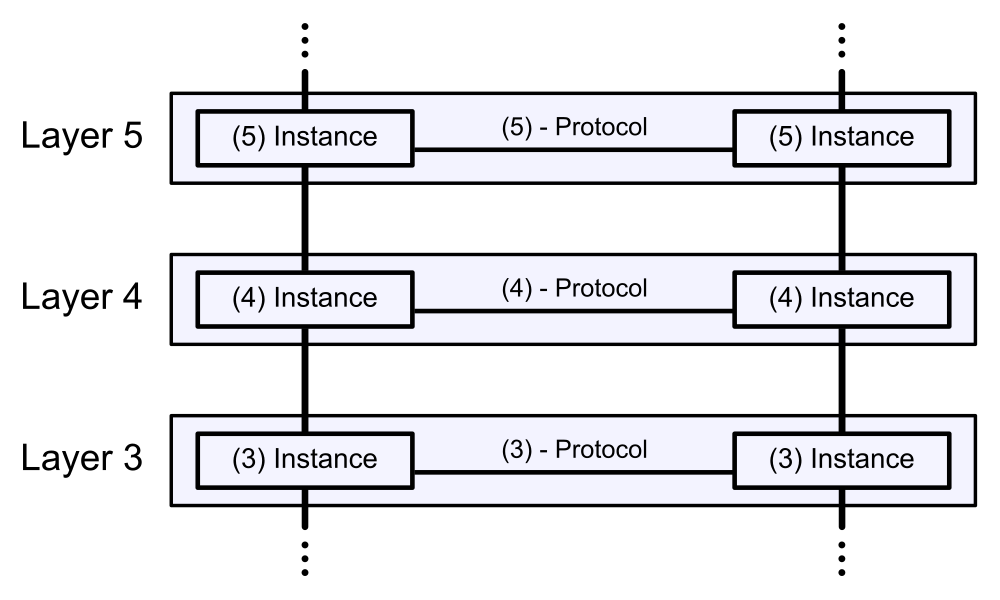
\includegraphics[width=\linewidth,height=0.70\textheight,keepaspectratio]{images-companion/ch15_osi.png}

\caption{Figure C15.1: Peer-Layer Protocol Communication — the OSI Model’s Layered Abstraction}

\end{figure}

\begin{figure}[H]

\hypertarget{fig-c15-2}{}\label{fig-c15-2}

\centering

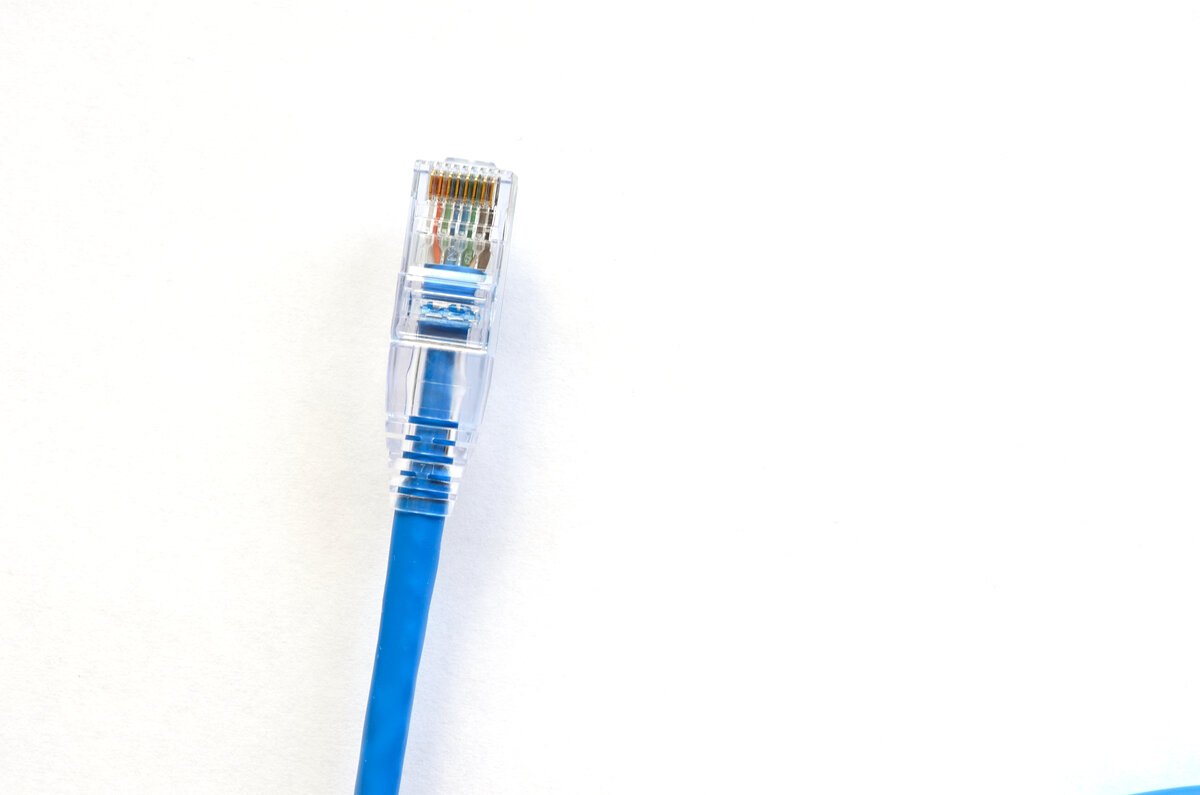
\includegraphics[width=\linewidth,height=0.70\textheight,keepaspectratio]{images-companion/ch15_copper.jpg}

\caption{Figure C15.2: Twisted-Pair Copper Ethernet Cable}

\end{figure}

\begin{figure}[H]

\hypertarget{fig-c15-3}{}\label{fig-c15-3}

\centering

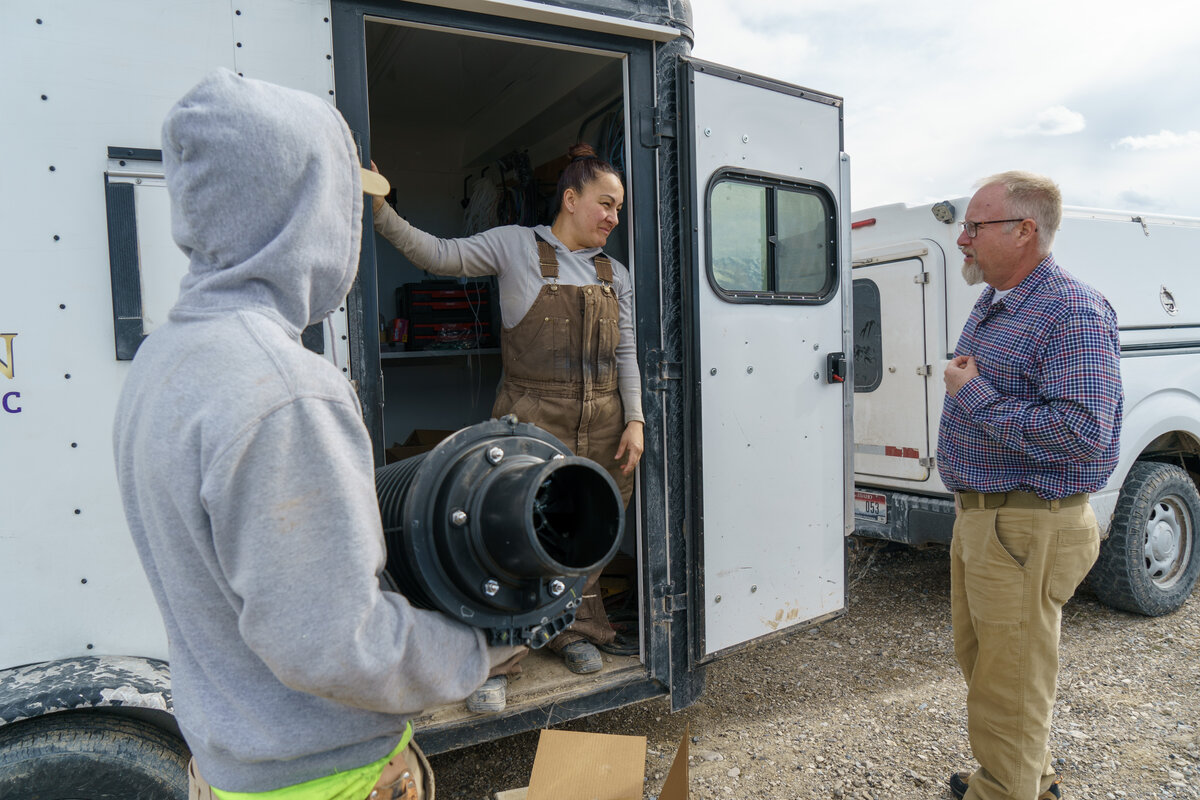
\includegraphics[width=\linewidth,height=0.70\textheight,keepaspectratio]{images-companion/ch15_fiber.jpg}

\caption{Figure C15.3: Installing Fiber-Optic Cabling for Rural Broadband (USDA Rural Development, 2024)}

\end{figure}

\begin{figure}[H]

\hypertarget{fig-c15-5}{}\label{fig-c15-5}

\centering

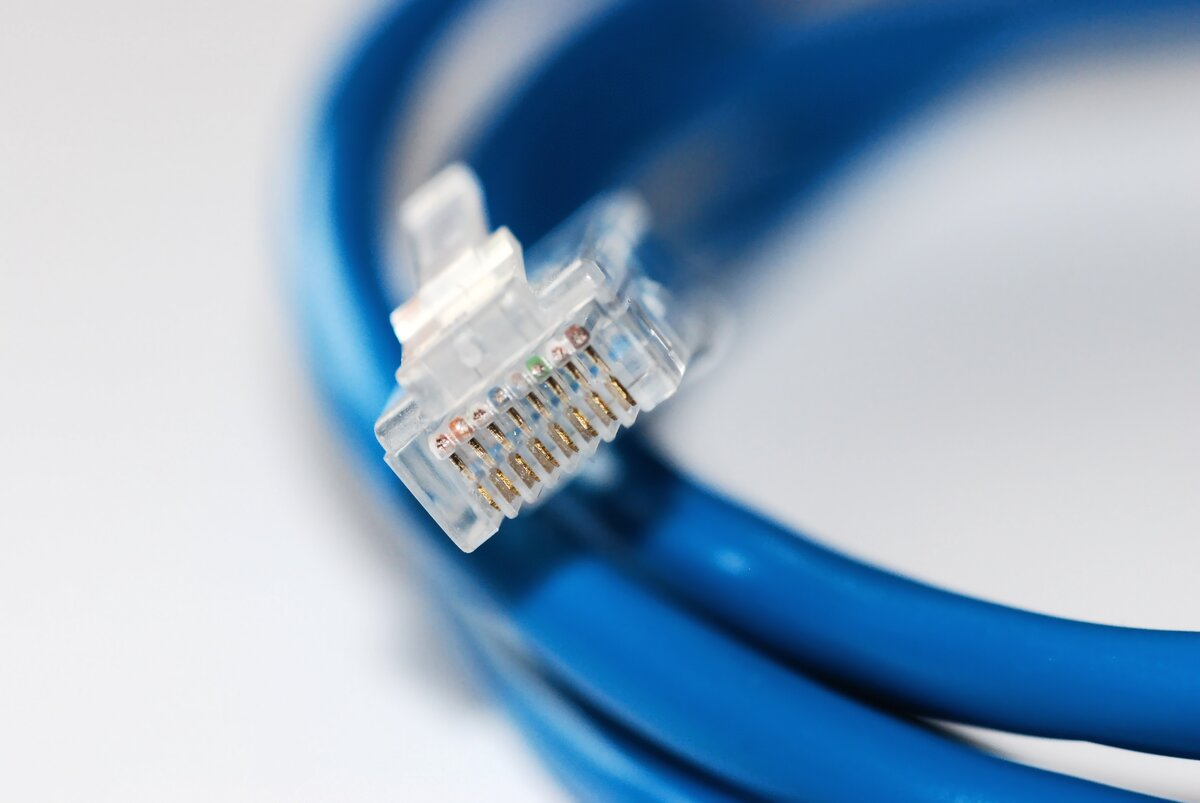
\includegraphics[width=\linewidth,height=0.70\textheight,keepaspectratio]{images-companion/ch15_ethernet.jpg}

\caption{Figure C15.5: RJ45 (8P8C) Connector Used for Ethernet Twisted-Pair Cabling}

\end{figure}

\begin{figure}[H]

\hypertarget{fig-c15-6}{}\label{fig-c15-6}

\centering

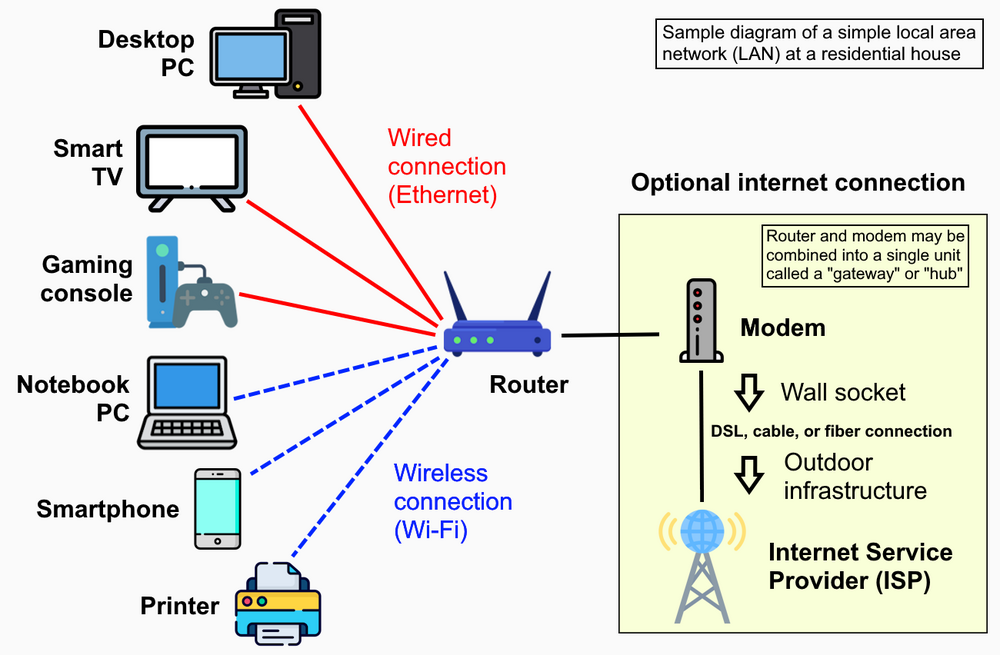
\includegraphics[width=\linewidth,height=0.70\textheight,keepaspectratio]{images-companion/ch15_ip.png}

\caption{Figure C15.6: Example Home LAN / IP Network Diagram}

\end{figure}

\begin{figure}[H]

\hypertarget{fig-c15-7}{}\label{fig-c15-7}

\centering

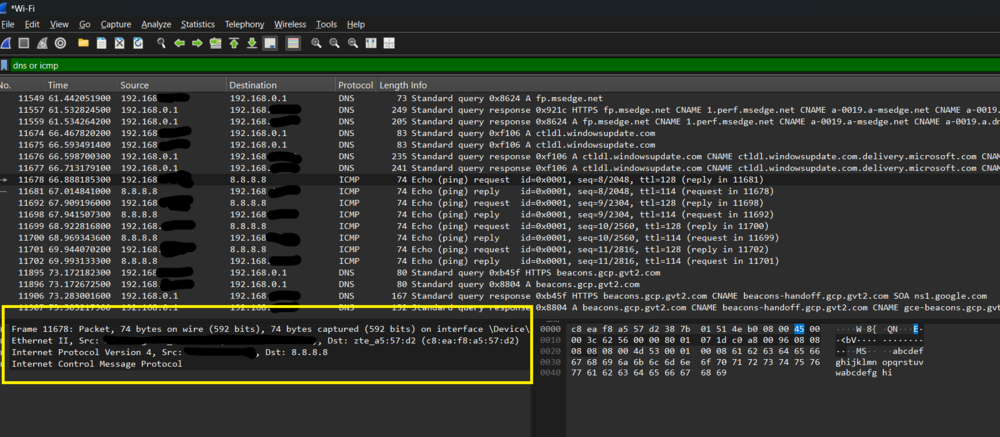
\includegraphics[width=\linewidth,height=0.70\textheight,keepaspectratio]{images-companion/ch15_transport.png}

\caption{Figure C15.7: Wireshark Packet Capture — Inspecting Transport/Network-Layer Protocol Traffic}

\end{figure}

\begin{figure}[H]

\hypertarget{fig-c15-8}{}\label{fig-c15-8}

\centering

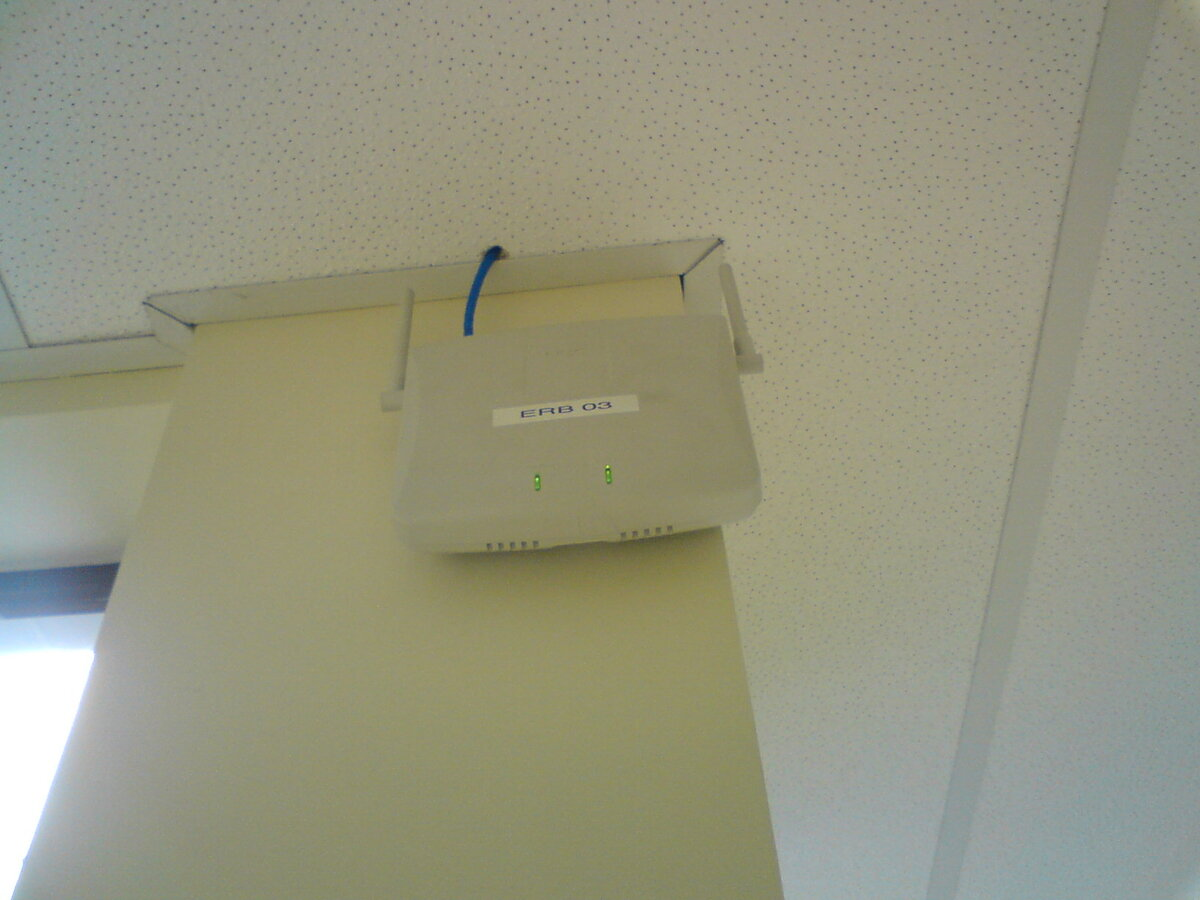
\includegraphics[width=\linewidth,height=0.70\textheight,keepaspectratio]{images-companion/ch15_wifi.jpg}

\caption{Figure C15.8: Ceiling-Mounted Wireless (Wi-Fi) Access Point}

\end{figure}

\begin{figure}[H]

\hypertarget{fig-c15-10}{}\label{fig-c15-10}

\centering

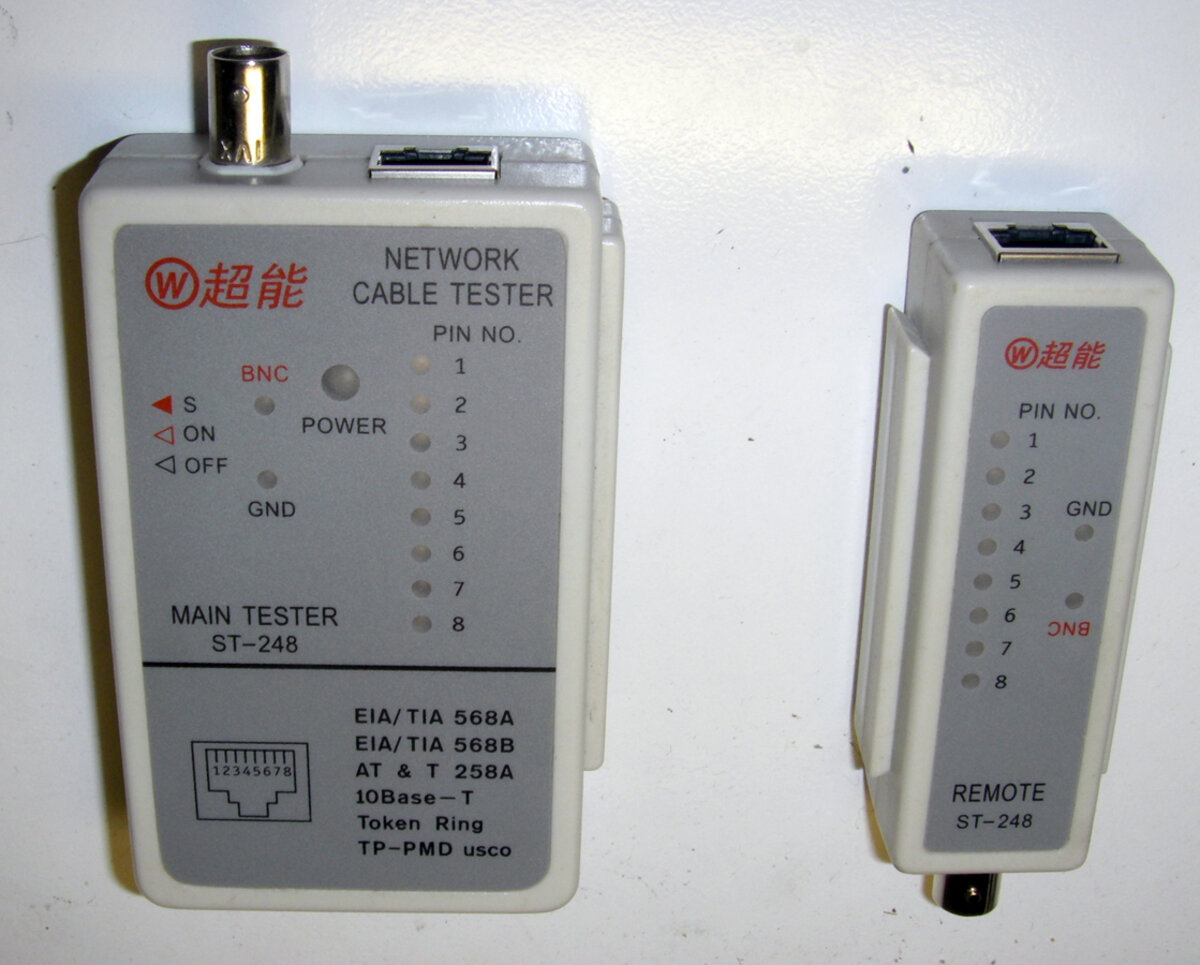
\includegraphics[width=\linewidth,height=0.70\textheight,keepaspectratio]{images-companion/ch15_perf.jpg}

\caption{Figure C15.10: Network Cable Tester — Verifying Link Performance and Wiring Continuity}

\end{figure}

\section{Chapter 16: Antenna Design and
Principles}\label{chapter-16-antenna-design-and-principles}

\begin{figure}[H]

\hypertarget{fig-c16-1}{}\label{fig-c16-1}

\centering

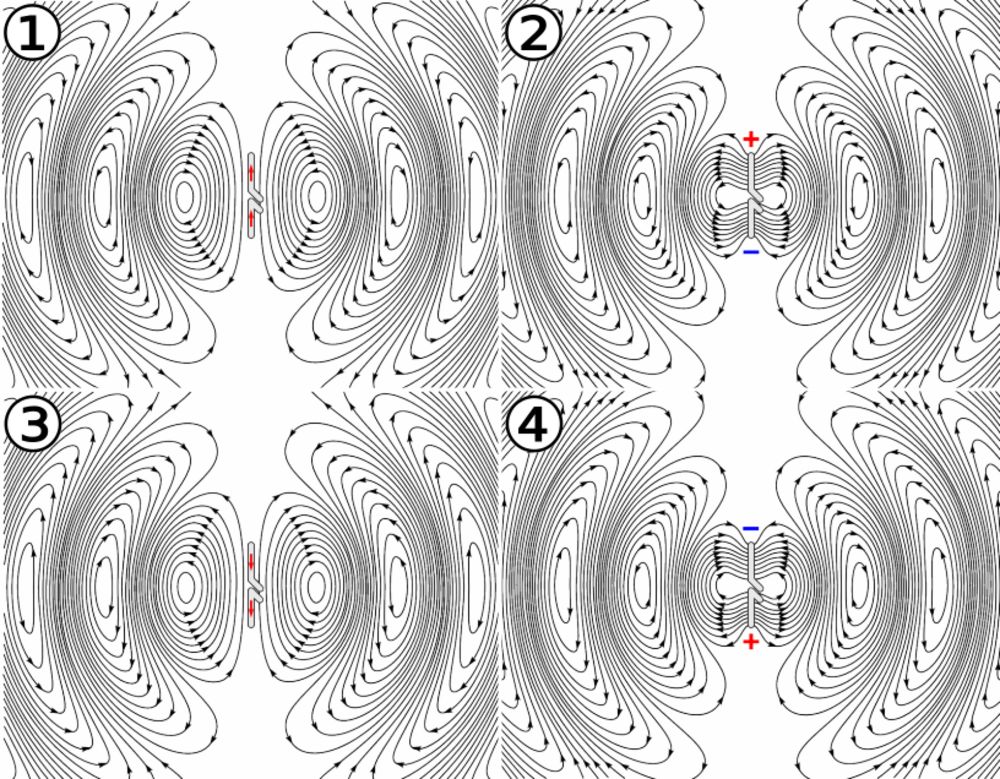
\includegraphics[width=\linewidth,height=0.70\textheight,keepaspectratio]{images-companion/ch16_fundamentals.png}

\caption{Figure C16.1: Half-Wave Dipole Antenna Field Patterns (Transmit and Receive)}

\end{figure}

\begin{figure}[H]

\hypertarget{fig-c16-2}{}\label{fig-c16-2}

\centering

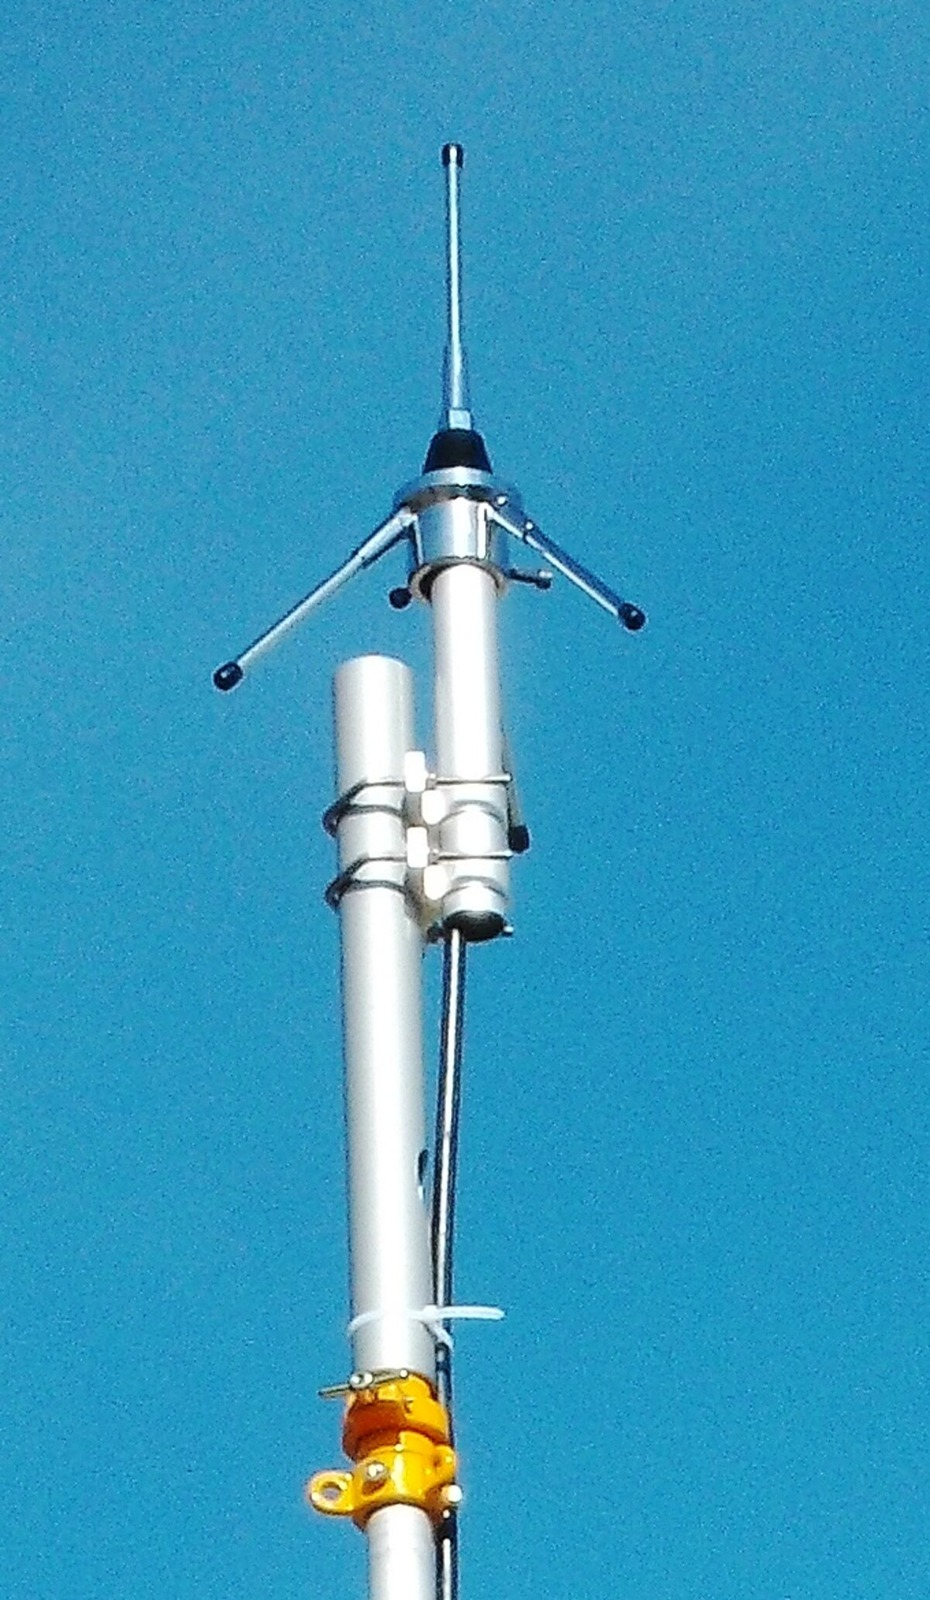
\includegraphics[width=\linewidth,height=0.70\textheight,keepaspectratio]{images-companion/ch16_wire.jpg}

\caption{Figure C16.2: UHF Ground-Plane (Quarter-Wave Whip) Antenna}

\end{figure}

\begin{figure}[H]

\hypertarget{fig-c16-3}{}\label{fig-c16-3}

\centering

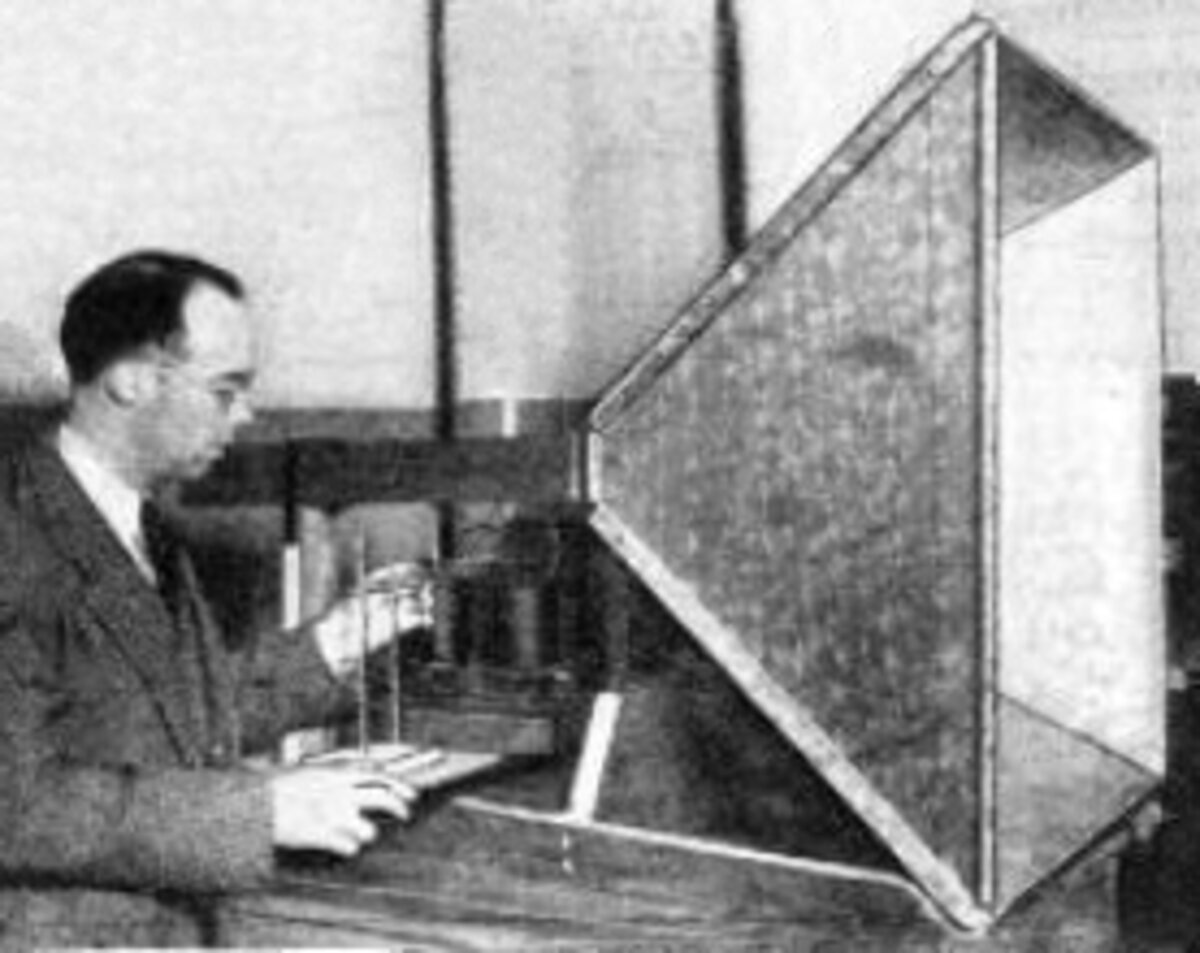
\includegraphics[width=\linewidth,height=0.70\textheight,keepaspectratio]{images-companion/ch16_aperture.jpg}

\caption{Figure C16.3: Wilmer Barrow and the First Modern Horn Antenna (1938)}

\end{figure}

\begin{figure}[H]

\hypertarget{fig-c16-5}{}\label{fig-c16-5}

\centering

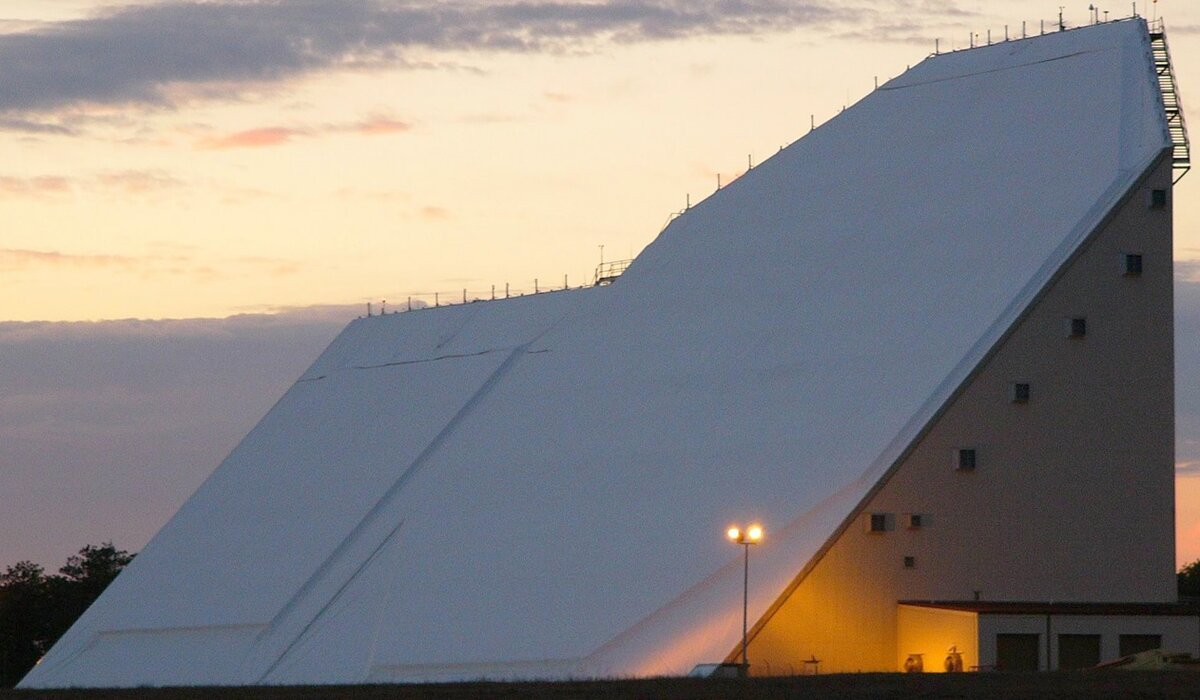
\includegraphics[width=\linewidth,height=0.70\textheight,keepaspectratio]{images-companion/ch16_arrays.jpg}

\caption{Figure C16.5: AN/FPS-85 Phased-Array Radar Antenna Building, Eglin AFB}

\end{figure}

\begin{figure}[H]

\hypertarget{fig-c16-6}{}\label{fig-c16-6}

\centering

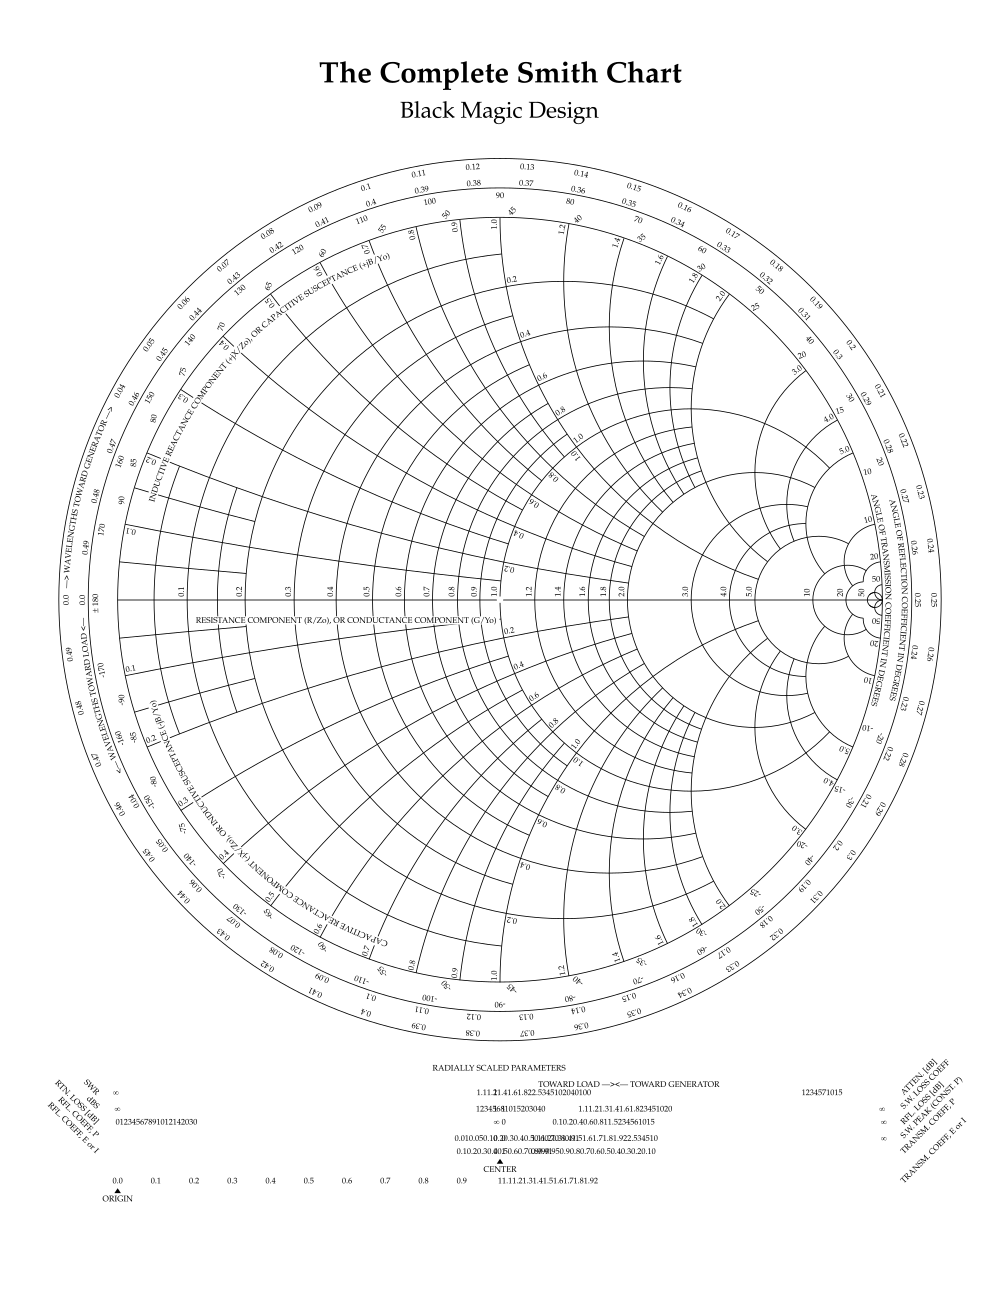
\includegraphics[width=\linewidth,height=0.70\textheight,keepaspectratio]{images-companion/ch16_matching.png}

\caption{Figure C16.6: Smith Chart Used for Antenna/Transmission-Line Impedance Matching}

\end{figure}

\section{Chapter 17: Radar Systems}\label{chapter-17-radar-systems}

\begin{figure}[H]

\hypertarget{fig-c17-3}{}\label{fig-c17-3}

\centering

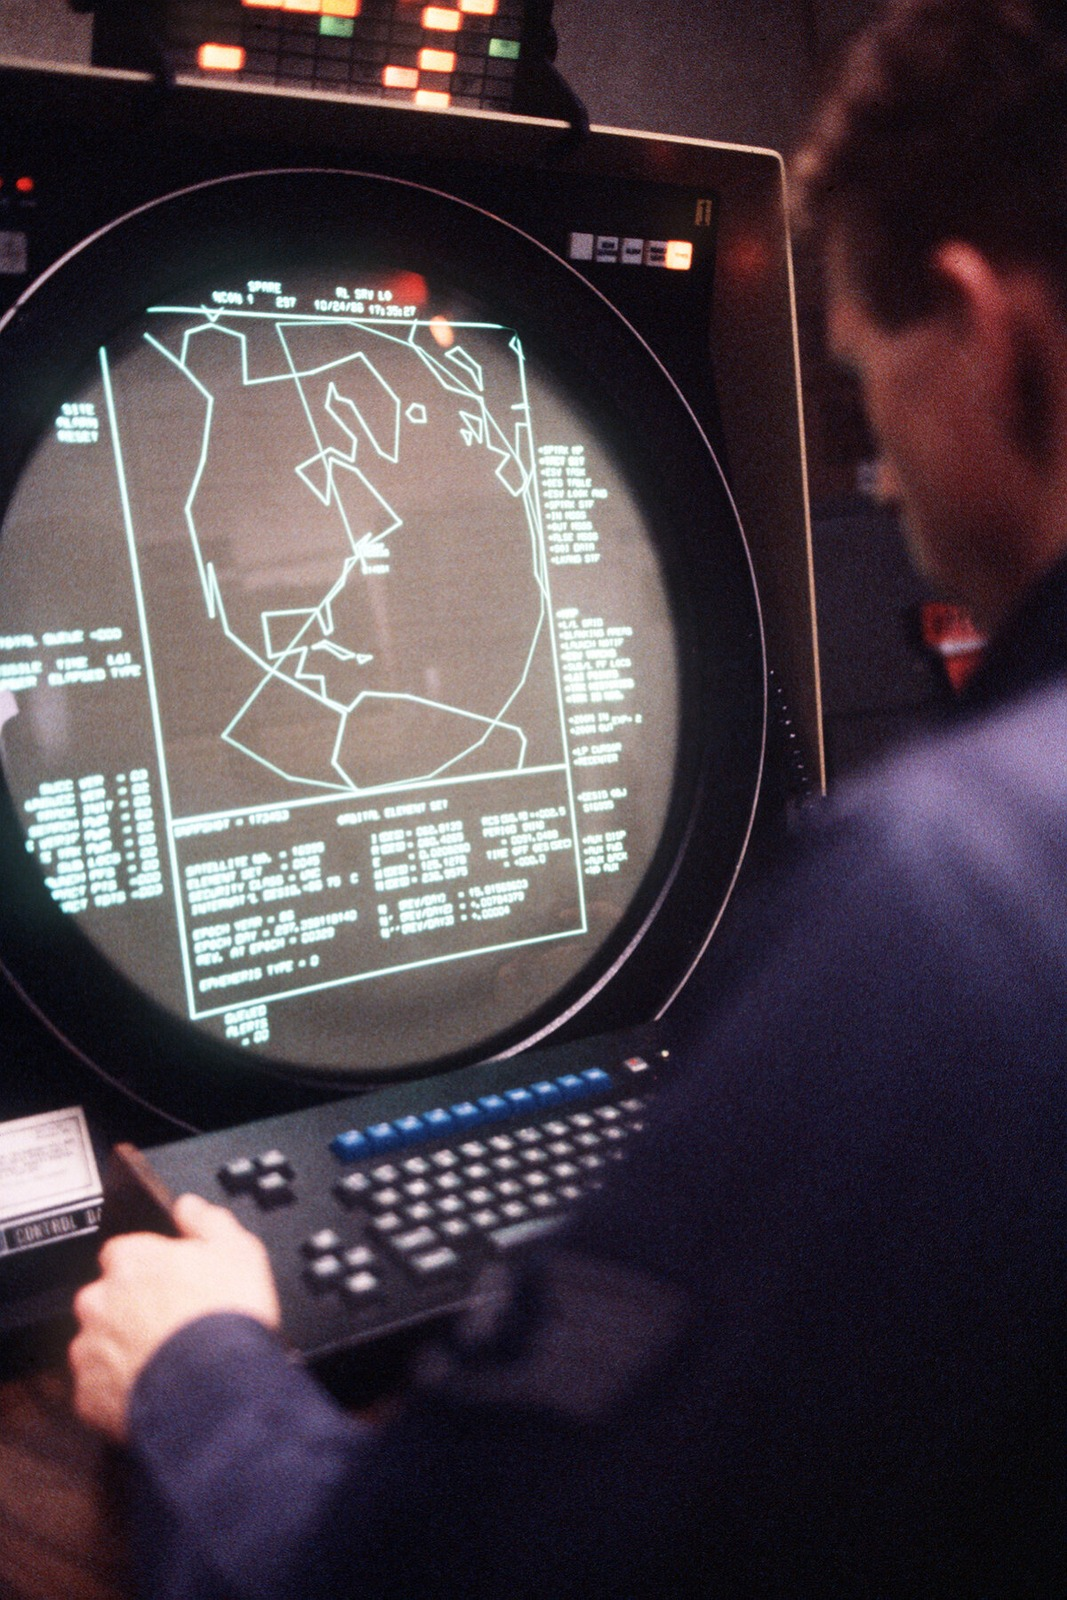
\includegraphics[width=\linewidth,height=0.70\textheight,keepaspectratio]{images-companion/ch17_sigproc.jpg}

\caption{Figure C17.3: PAVE PAWS Radar Operator Console — Processed Track Display}

\end{figure}

\begin{figure}[H]

\hypertarget{fig-c17-4}{}\label{fig-c17-4}

\centering

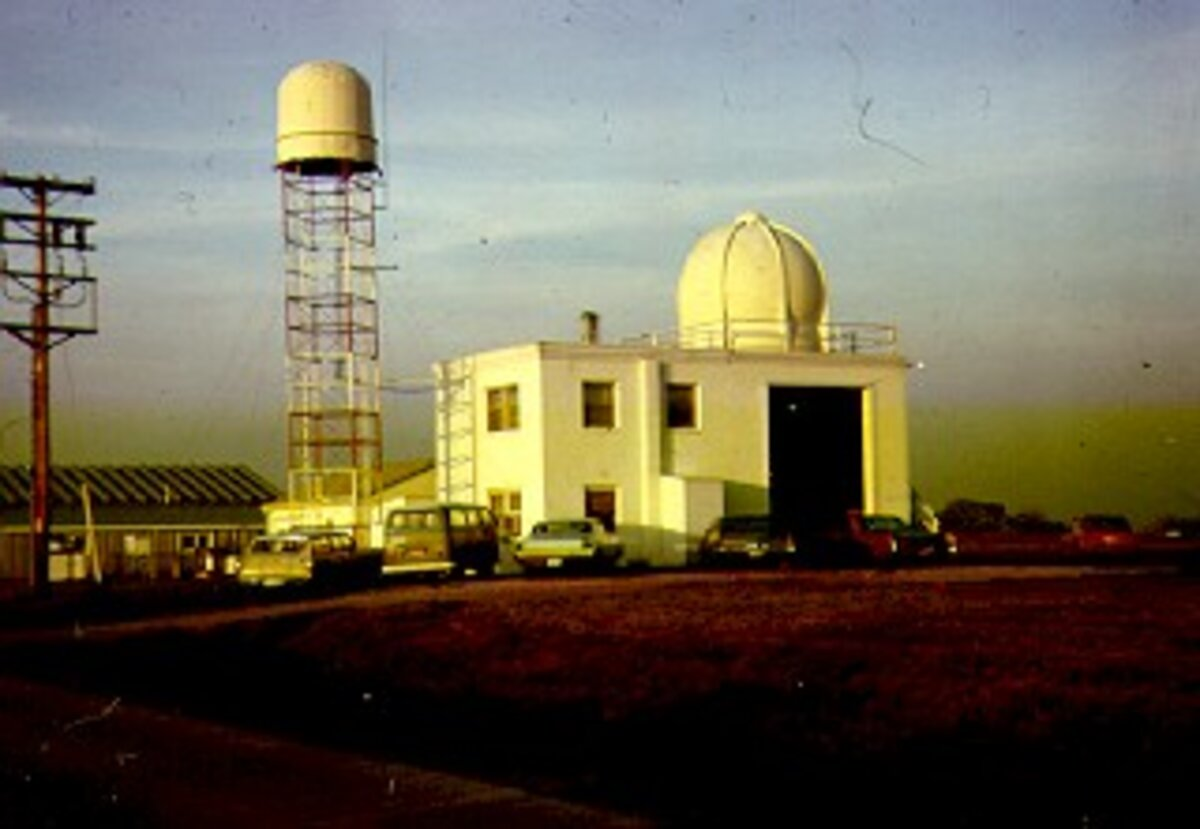
\includegraphics[width=\linewidth,height=0.70\textheight,keepaspectratio]{images-companion/ch17_applications.jpg}

\caption{Figure C17.4: WSR-1 Weather Radar and Radiosonde Dome, North Omaha Airport}

\end{figure}

\begin{figure}[H]

\hypertarget{fig-c17-5}{}\label{fig-c17-5}

\centering

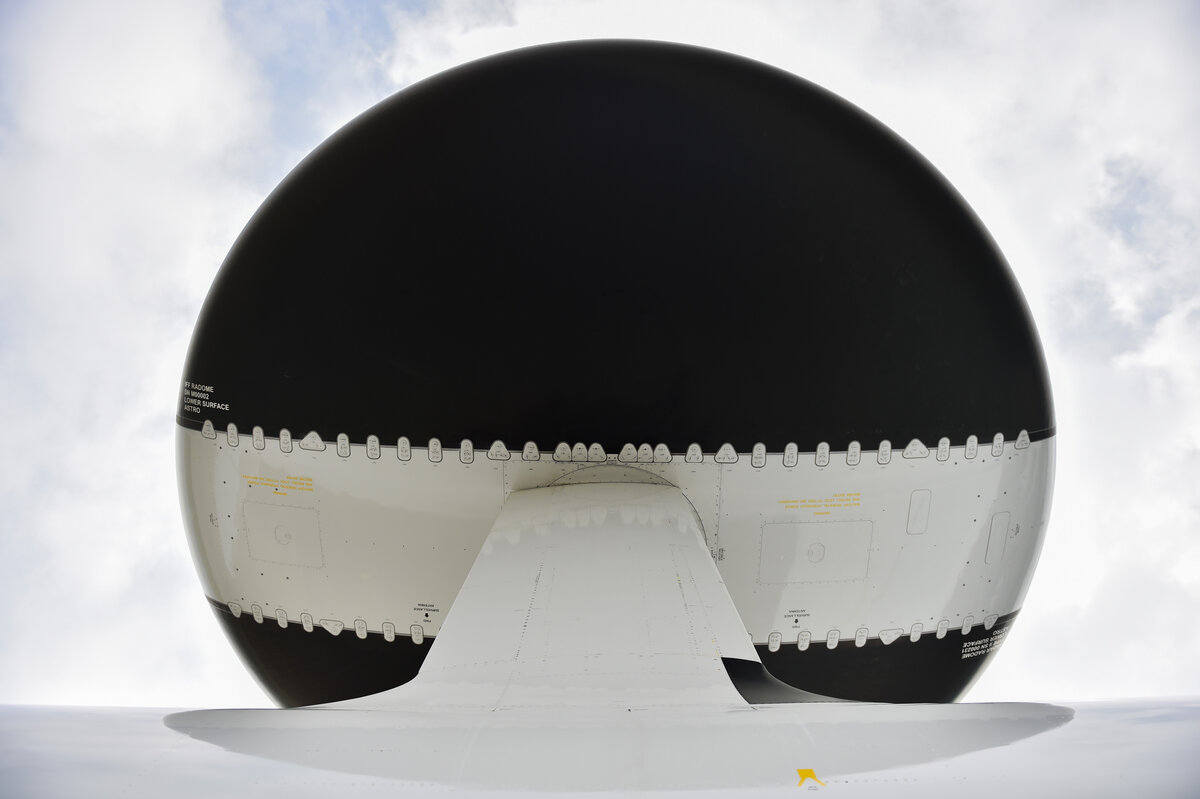
\includegraphics[width=\linewidth,height=0.70\textheight,keepaspectratio]{images-companion/ch17_comparison.jpg}

\caption{Figure C17.5: NATO E-3 AWACS — Airborne Early-Warning Radar System}

\end{figure}

\section{Chapter 18: Optics}\label{chapter-18-optics}

\begin{figure}[H]

\hypertarget{fig-c18-1}{}\label{fig-c18-1}

\centering

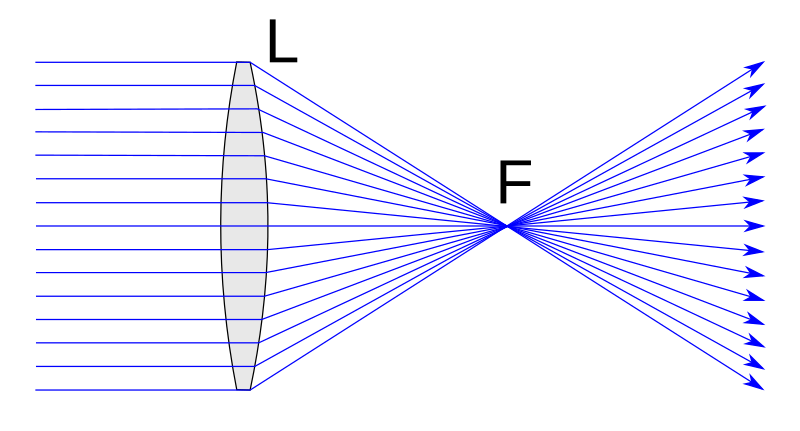
\includegraphics[width=\linewidth,height=0.70\textheight,keepaspectratio]{images-companion/ch18_geometric.png}

\caption{Figure C18.1: Ray Diagram Through a Perfect Convex (Converging) Lens}

\end{figure}

\begin{figure}[H]

\hypertarget{fig-c18-2}{}\label{fig-c18-2}

\centering

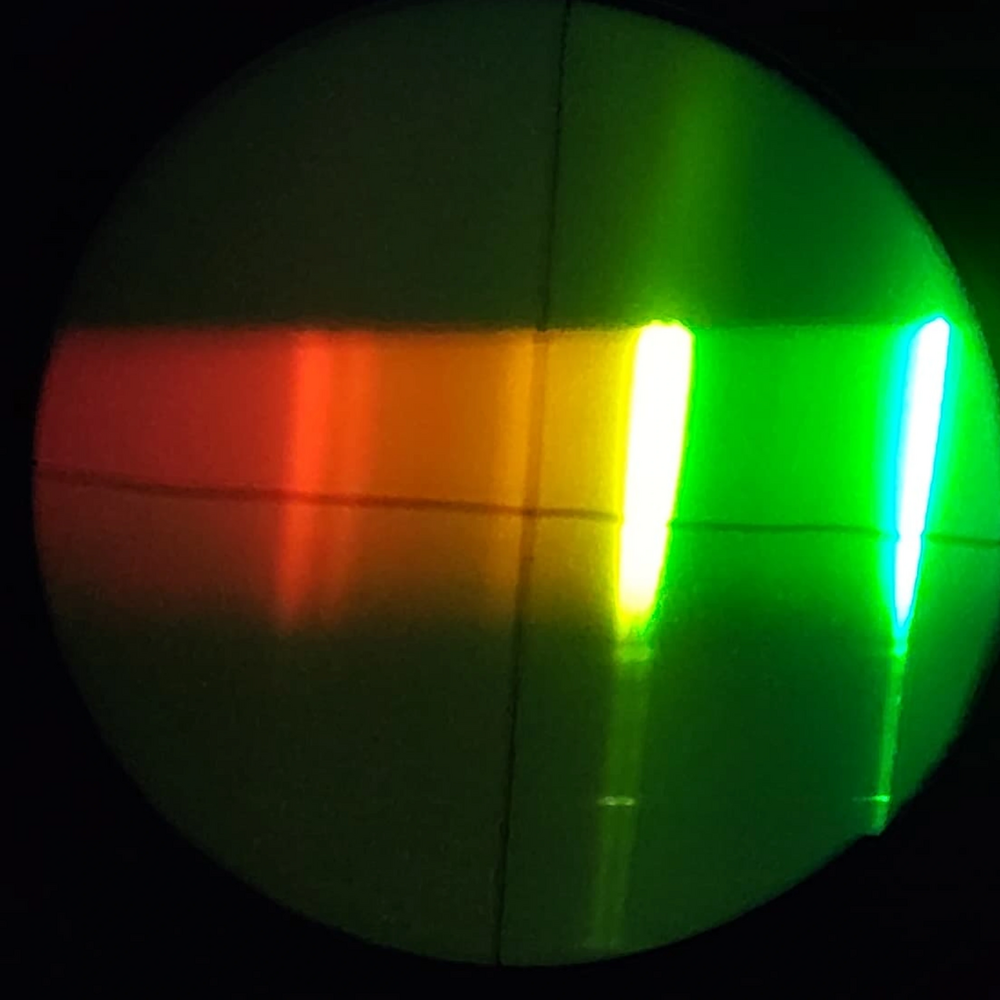
\includegraphics[width=\linewidth,height=0.70\textheight,keepaspectratio]{images-companion/ch18_wave.png}

\caption{Figure C18.2: Emission Spectrum Resolved by a Diffraction Grating}

\end{figure}

\begin{figure}[H]

\hypertarget{fig-c18-3}{}\label{fig-c18-3}

\centering

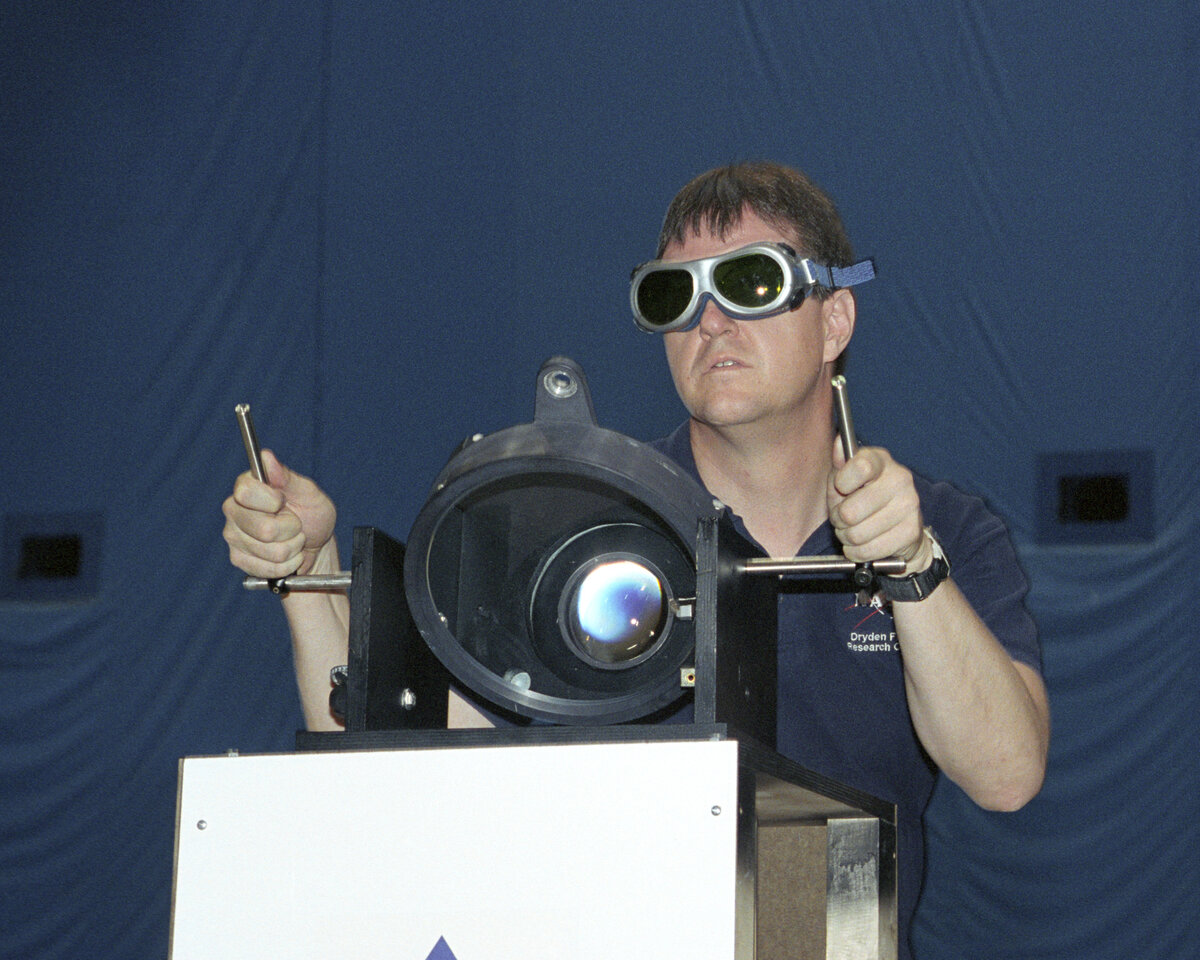
\includegraphics[width=\linewidth,height=0.70\textheight,keepaspectratio]{images-companion/ch18_lasers.jpg}

\caption{Figure C18.3: NASA Researcher Aligning a Laser Device for a Laser-Powered Model Aircraft Demonstration}

\end{figure}

\begin{figure}[H]

\hypertarget{fig-c18-4}{}\label{fig-c18-4}

\centering

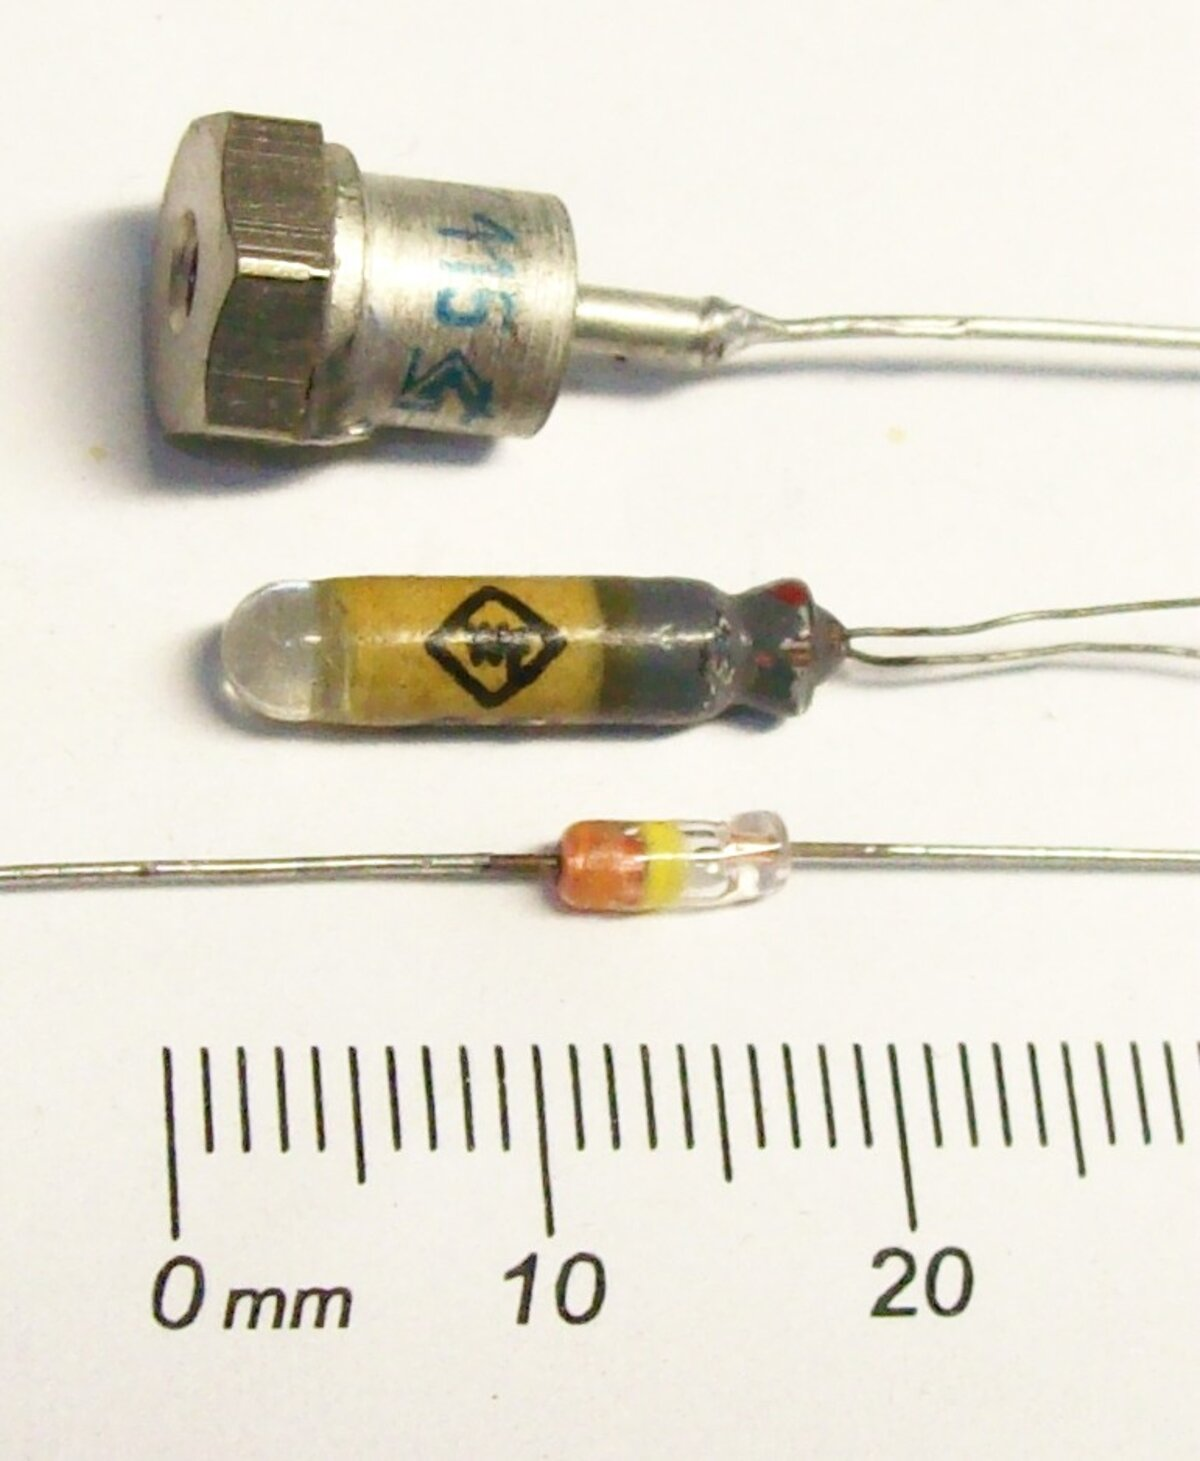
\includegraphics[width=\linewidth,height=0.70\textheight,keepaspectratio]{images-companion/ch18_photodetectors.jpg}

\caption{Figure C18.4: Germanium Photodiode}

\end{figure}

\begin{figure}[H]

\hypertarget{fig-c18-6}{}\label{fig-c18-6}

\centering

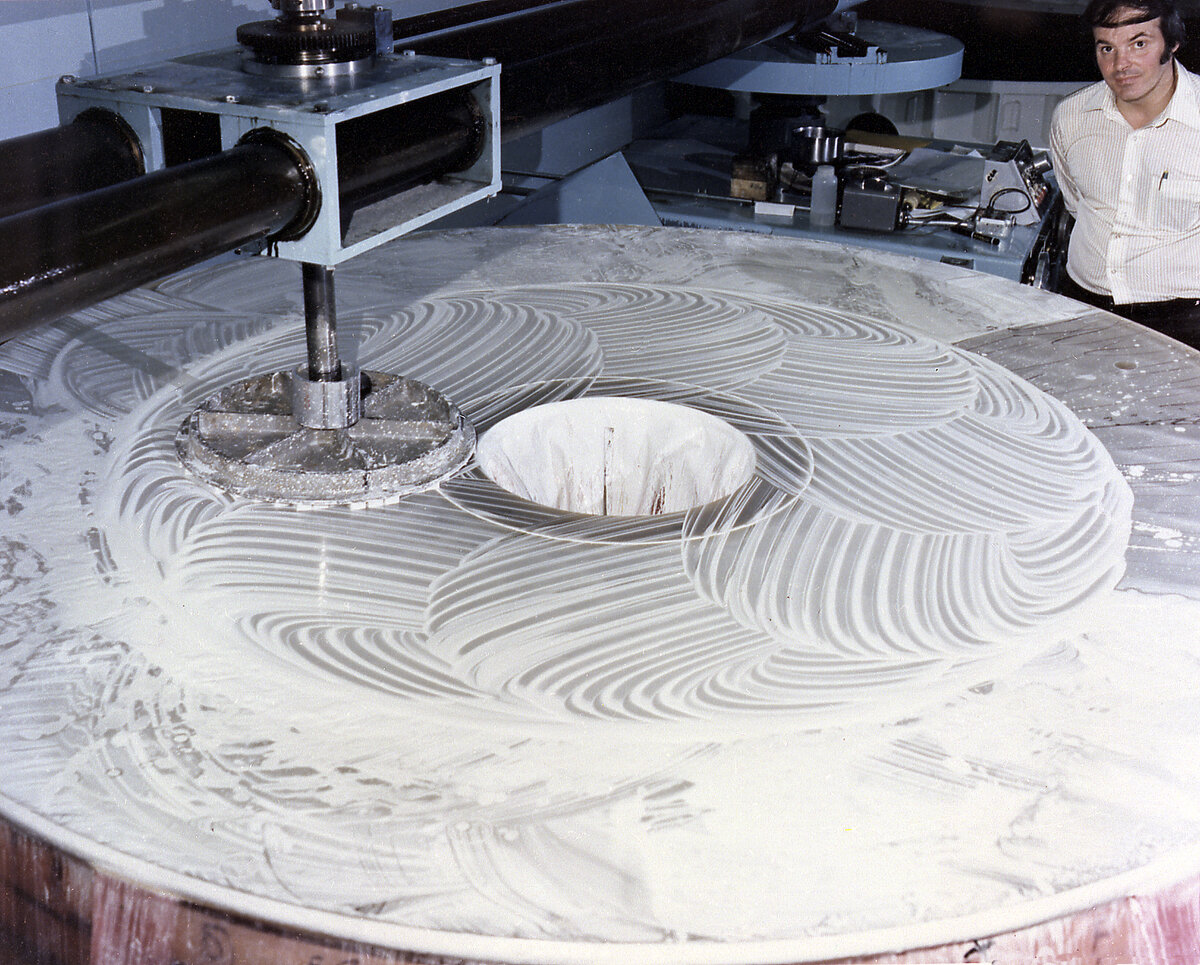
\includegraphics[width=\linewidth,height=0.70\textheight,keepaspectratio]{images-companion/ch18_systemdesign.jpg}

\caption{Figure C18.6: Hubble Space Telescope Primary Mirror — a Precision Optical System}

\end{figure}

\section{Chapter 19: Engineering
Economics}\label{chapter-19-engineering-economics}

\begin{figure}[H]

\hypertarget{fig-c19-11}{}\label{fig-c19-11}

\centering

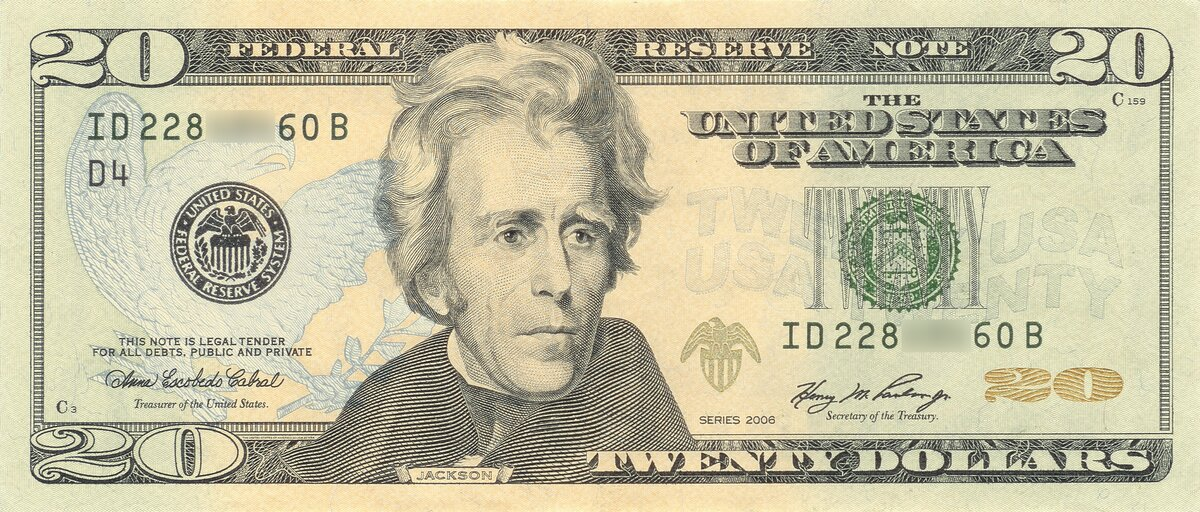
\includegraphics[width=\linewidth,height=0.70\textheight,keepaspectratio]{images-companion/ch19_inflation.jpg}

\caption{Figure C19.11: U.S. Currency — Illustrating Purchasing Power and Inflation}

\end{figure}

\section{Appendix A: Imaginary Numbers and
Phasors}\label{appendix-a-imaginary-numbers-and-phasors}

\begin{figure}[H]

\hypertarget{fig-ca-4}{}\label{fig-ca-4}

\centering

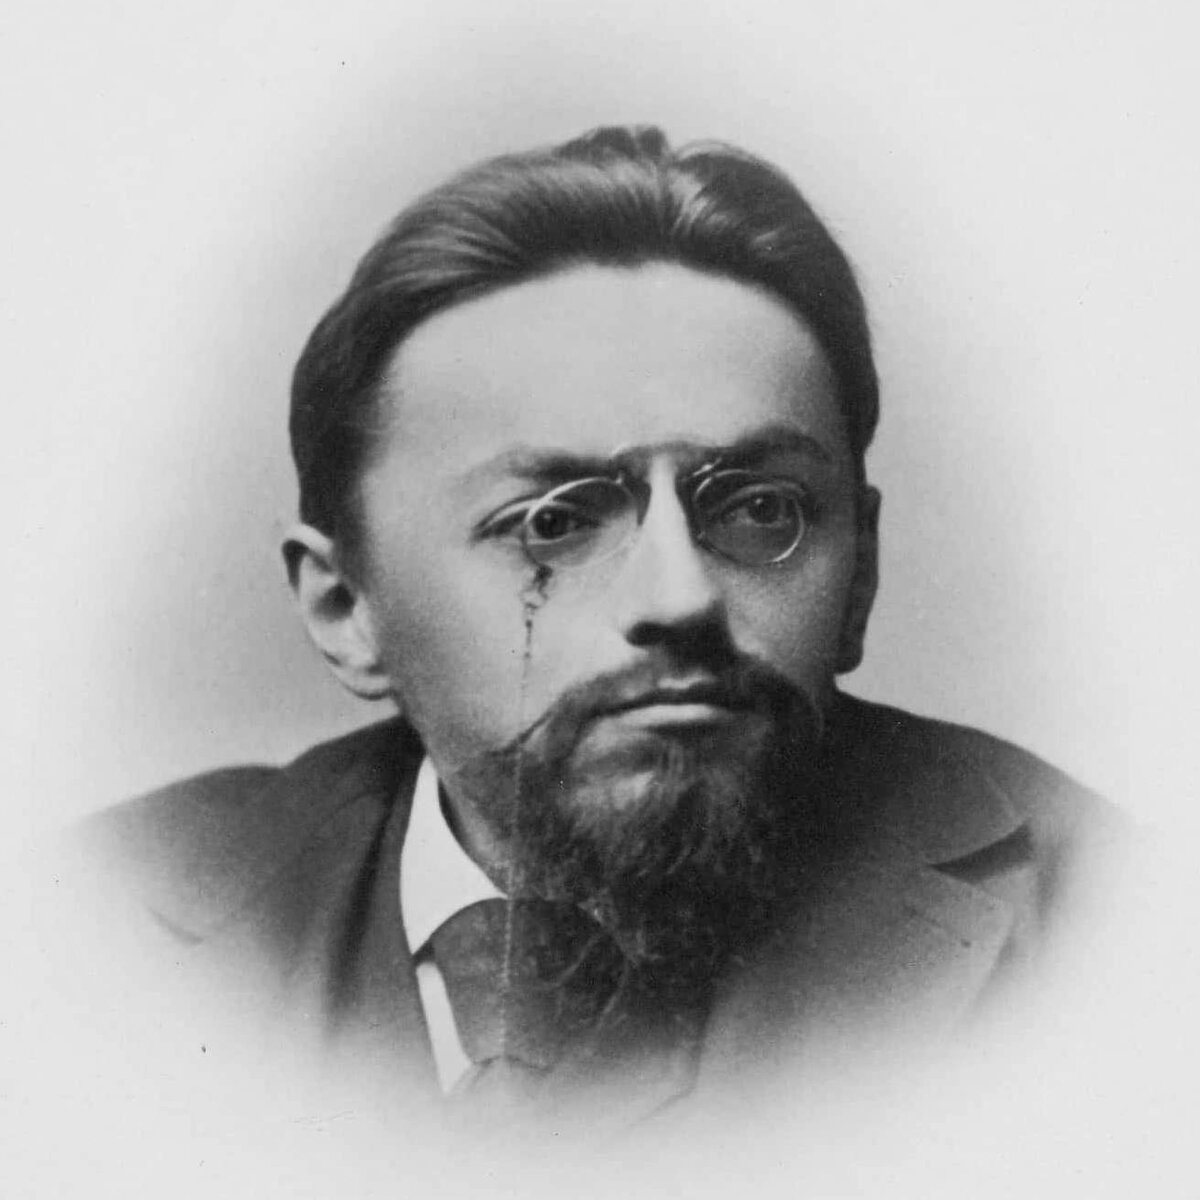
\includegraphics[width=\linewidth,height=0.70\textheight,keepaspectratio]{images-companion/appa_phasors.jpg}

\caption{Figure CA.4: Charles Proteus Steinmetz, Pioneer of the Phasor Method for AC Circuit Analysis}

\end{figure}

\section{Appendix B: Arctangent and
atan2}\label{appendix-b-arctangent-and-atan2}

\section{Appendix C: Decibels}\label{appendix-c-decibels}

\begin{figure}[H]

\hypertarget{fig-cc-1}{}\label{fig-cc-1}

\centering

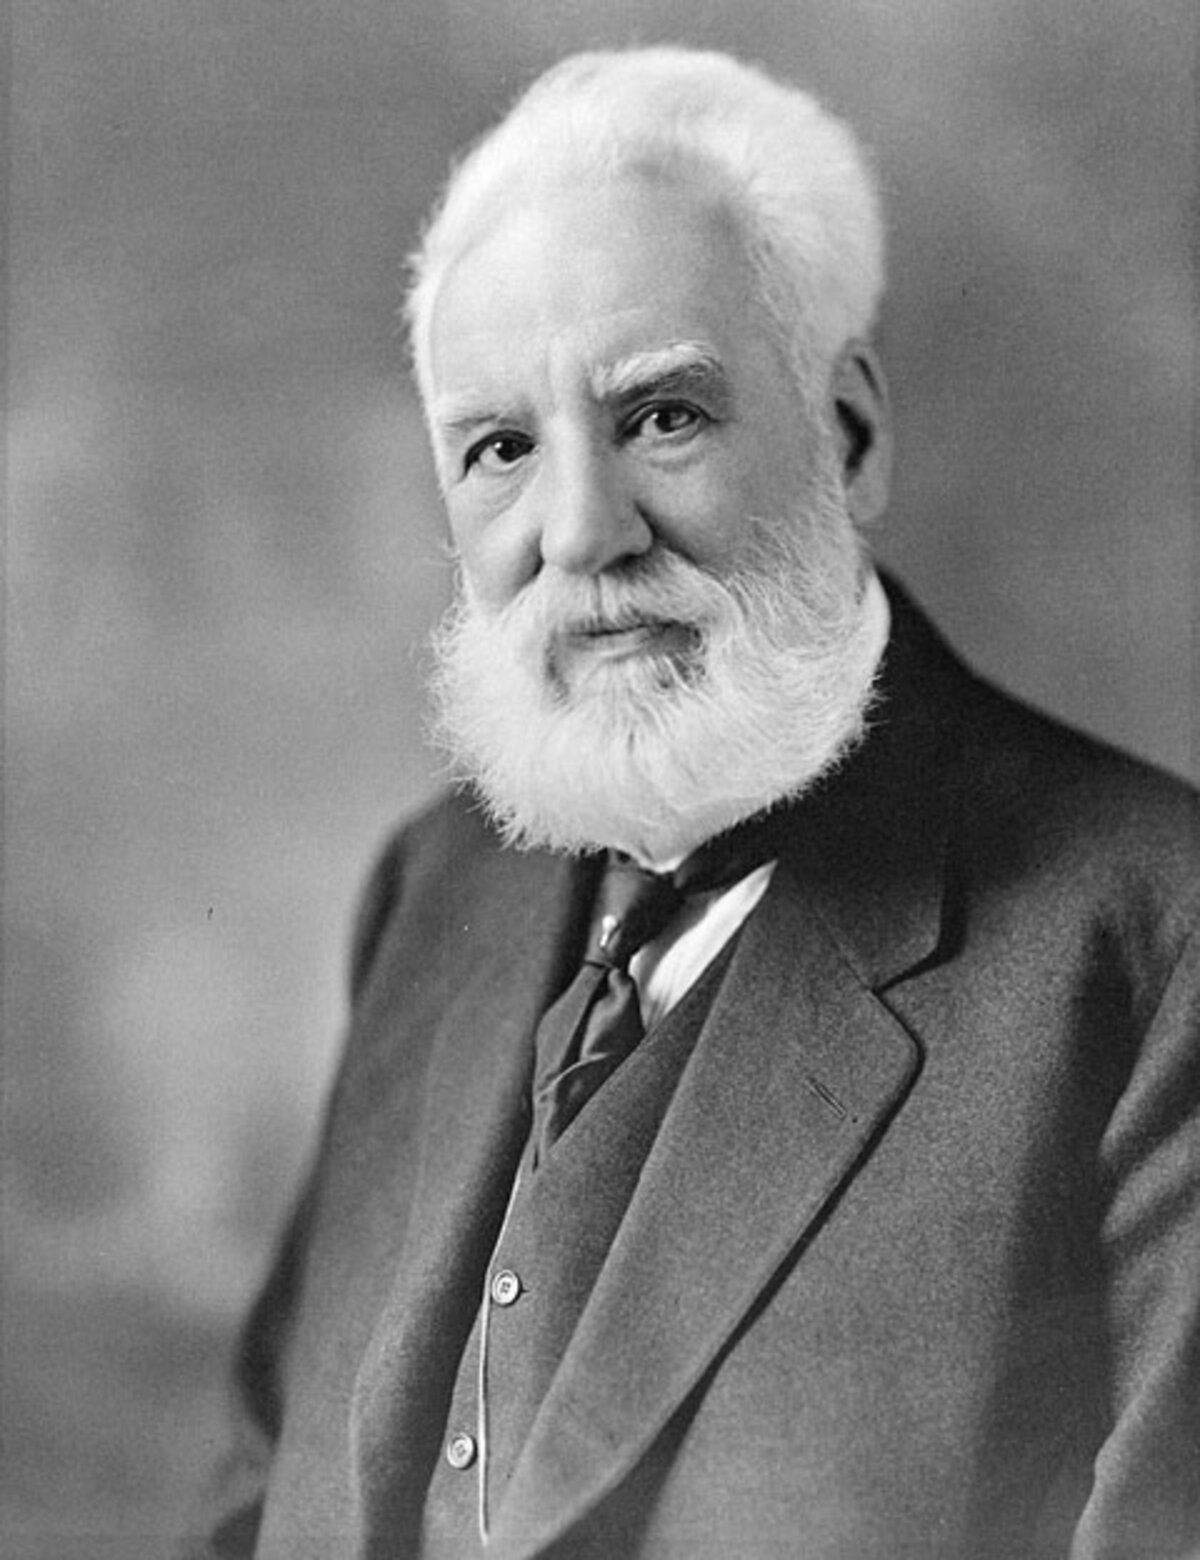
\includegraphics[width=\linewidth,height=0.70\textheight,keepaspectratio]{images-companion/appc_decibels.jpg}

\caption{Figure CC.1: Alexander Graham Bell, Namesake of the Bel/Decibel}

\end{figure}

\section{Appendix D: Unit Prefixes and SI
Units}\label{appendix-d-unit-prefixes-and-si-units}

\begin{figure}[H]

\hypertarget{fig-cd-1}{}\label{fig-cd-1}

\centering

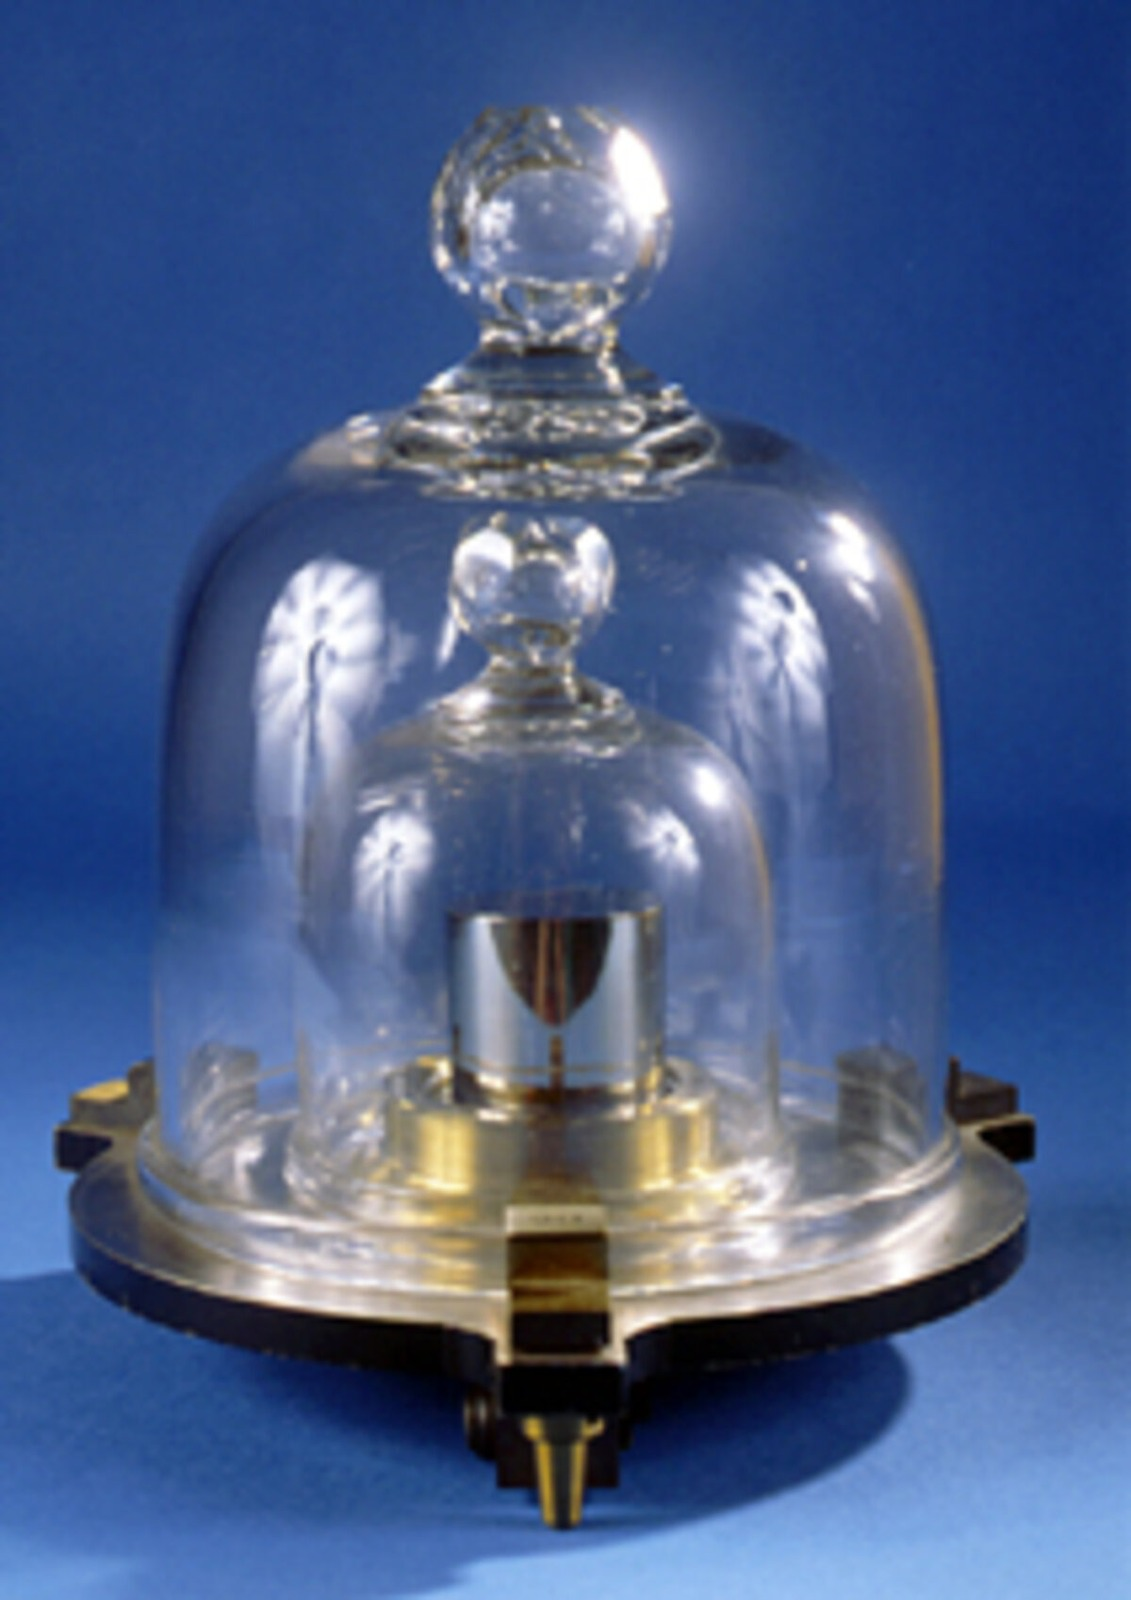
\includegraphics[width=\linewidth,height=0.70\textheight,keepaspectratio]{images-companion/appd_units.jpg}

\caption{Figure CD.1: U.S. National Prototype Kilogram K20 — a Historical SI Base Unit Standard}

\end{figure}

\section{Appendix E: Getting Started with Python and
marimo}\label{appendix-e-getting-started-with-python-and-marimo}

\section{Appendix F: Matrix
Operations}\label{appendix-f-matrix-operations}

\section{Appendix G: TCLab Control
Lab}\label{appendix-g-tclab-control-lab}

\end{document}
